\chapter{Radiation Damage to the ATLAS Pixel Detector}
\label{chap:digi}

The goal of this Chapter is to present a model for radiation damage to silicon sensors that is fast enough to be incorporated directly into the simulation of \textit{digitization}: the conversion from energy depositions from charged particles to digital signals sent from module front ends to the detector readout system.  Figure~\ref{fig:atlassim} shows the flowchart of the ATLAS Monte Carlo simulation, from 
event generation to analysis; digitization step intervenes before reconstruction.


\begin{figure}[!htpb]
\centering
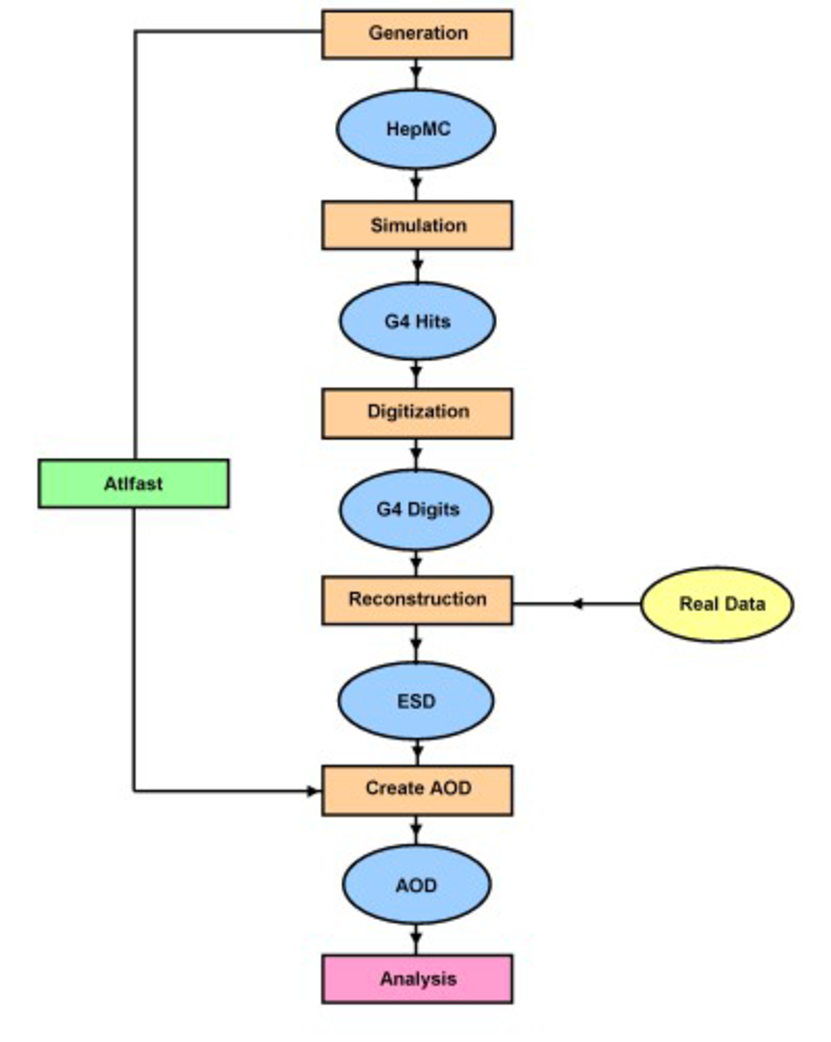
\includegraphics[height=0.45\textheight]{atlassim.pdf}
\caption{\label{fig:atlassim}Flowchart of Monte Carlo simulation in ATLAS.}
\end{figure}

 
After introducing the motivations and the the fluences predictions for the actual detector in 
Section~\ref{sec:expflu}, a model of charge deposition and measurement that includes radiation 
damage effects is documented in Section~\ref{sec:fullmodel}. Comparisons of the models with data are 
presented in Setion~\ref{sec:digivalidation}; conclusions and plans will be drawn in Section~\ref{sec:digiconclusions}.


\section{Expected Fluence for the ATLAS Pixel Detector}
\label{sec:expflu}
As discussed previously in this Section, silicon pixel detectors are at 
the core of the current ATLAS  experiment.  Given their close proximity to the interaction point, these 
detectors are subjected to an 
unprecedented amount of radiation over their lifetime:  the innermost layers will receive 
fluences in excess of $10^{15}$ 1 MeV $n_\text{eq}/\text{cm}^2$. The modules comprising the detector are designed to be as radiation tolerant as possible, but their performance will still degrade over time.  It is therefore critical to model the impact of radiation damage for an accurate simulation of charged particle interactions with the detector and the reconstruction of their trajectories.  Modelling radiation damage effects is especially relevant for the high luminosity upgrade of the LHC (HL-LHC - see also Chapter~\ref{chap:ITk}); the instantaneous and integrated luminosity will exceed current values by a factor of 100.  The simulations for the present and future ATLAS detectors currently do not model the effect of radiation damage on the silicon sensors of the Pixel detector~\cite{Aad:2010ah,ATL-PHYS-PUB-2016-025}
Section
As already discussed in~\ref{sec:RadDam}, radiation damage in silicon occurs from both ionising and 
non-ionizing energy losses. Ionizing radiation leads to an accumulation of charge in the silicon dioxide 
(SiO$_2$) and charge trapping at the SiO$_2$-Si interface~\cite{Oldham}, affecting in particular the 
readout electronics. However, the focus of this paper is bulk damage in the sensor due to non-ionising 
radiation~\cite{moll-thesis}.   Non-ionising radiation introduces defects into the sensor, which create 
energy levels in the band gap.  When occupied, these states lead to three macroscopic detector effects: 
a change the effective doping concentration, reduced signal collection efficiency due to charge trapping, 
and an increase in sensor leakage current. The change in effective doping concentration has 
consequences for the depletion voltage and electric field profile. For the pixel planar sensor before 
radiation, the depletion region grows from the backside of the sensor towards the pixel $n^+$ implant. 
After irradiation, the effective doping concentration decreases until the sensor bulk undergoes space 
charge sign inversion (often called \textit{type inversion}) from $n$-type to $p$-type. After this type 
inversion, the depletion region grows from the pixel implant towards the back side of the sensor and the 
depletion voltage gradually increases with further irradiation (more details in 
Section~\ref{sec:depletionvoltage}). The IBL underwent type inversion after about 3 fb$^{-1}$ of data 
collected in 2015 and the second innermost layer ($b$-layer) inverted in the 2012 run after about 
5-10~fb$^{-1}$. The effective doping concentration is further complicated by annealing in which new 
defects are formed or existing defects dissociate due to their thermal motion within the silicon lattice. As 
a result, radiation damage effects depend on both the irradiation and temperature 
history~\cite{moll-thesis}. 

 Complex radiation fields are simulated by 
propagating inelastic proton-proton interactions, generated by 
Pythia 8~\cite{Sjostrand:2006za,Sjostrand:2014zea} using the MSTW2008LO parton distribution 
functions~\cite{Martin:2009iq} and the A2 tune~\cite{ATLAS:2012uec}, through the ATLAS detector 
material using the particle transport code FLUKA~\cite{Battistoni:2007zzb,Ferrari:898301}. It is 
important to model as accurately as possible all the inner detector and calorimeter geometry details as 
high energy hadron cascades in the material lead to increased particle fluences in the inner detector, 
especially neutrons. A description of the ATLAS FLUKA simulation framework can be found 
in~\cite{Baranov:814823}.

Predictions of the 1 MeV neutron-equivalent fluences per fb$^{-1}$ in the ATLAS FLUKA inner detector 
geometry are shown in Figure~\ref{fig:fluenceoverview2}. The dominant contribution is from charged 
pions originating directly from the proton-proton collisions. The average values for the four pixel layers 
starting from the innermost one are $6.1\times 10^{12}$, $2.9\times 10^{12}$, $1.2\times 10^{12}$ 
and $7.8\times 10^{11}$ $n_\text{eq}/\text{cm}^2$, respectively. Safety factors have not been applied to 
these numbers.  The simulations predict some variation as a function of $z$.  For example, in the IBL 
the maximum predicted value of $6.6\times 10^{12}$ $n_\text{eq}/\text{cm}^2$ in the central location is 
about $10\%$ higher than the end regions (studied further in Section~\ref{sec:fluence}). 
Figure~\ref{fig:fluenceoverview} shows the same 1 MeV neutron-equivalent fluence normalised to 
delivered luminosity and displayed as a function of time and integrated luminosity. The luminosity is 
determined by a set of dedicated bunch-by-bunch luminosity detectors~\cite{Aaboud:2016hhf} that are 
calibrated using the van-der-Meer beam-separation method~\cite{vanderMeer:296752}.

By the end of the proton-proton collision runs in 2016, the IBL and $b$-layer had received integrated 
fluences approximately $\Phi=2\times 10^{14}$ $n_\text{eq}/\text{cm}^{2}$. Because the fluence 
decreases with distance, the outer two layers were exposed to less than half the fluence of the inner 
layers. The projected fluence on the IBL at the end of the LHC (300 fb$^{-1}$) is about 
$\Phi=2\times 10^{15}$ $n_\text{eq}/\text{cm}^{2}$. 

\begin{figure}[htpb!]
\centering
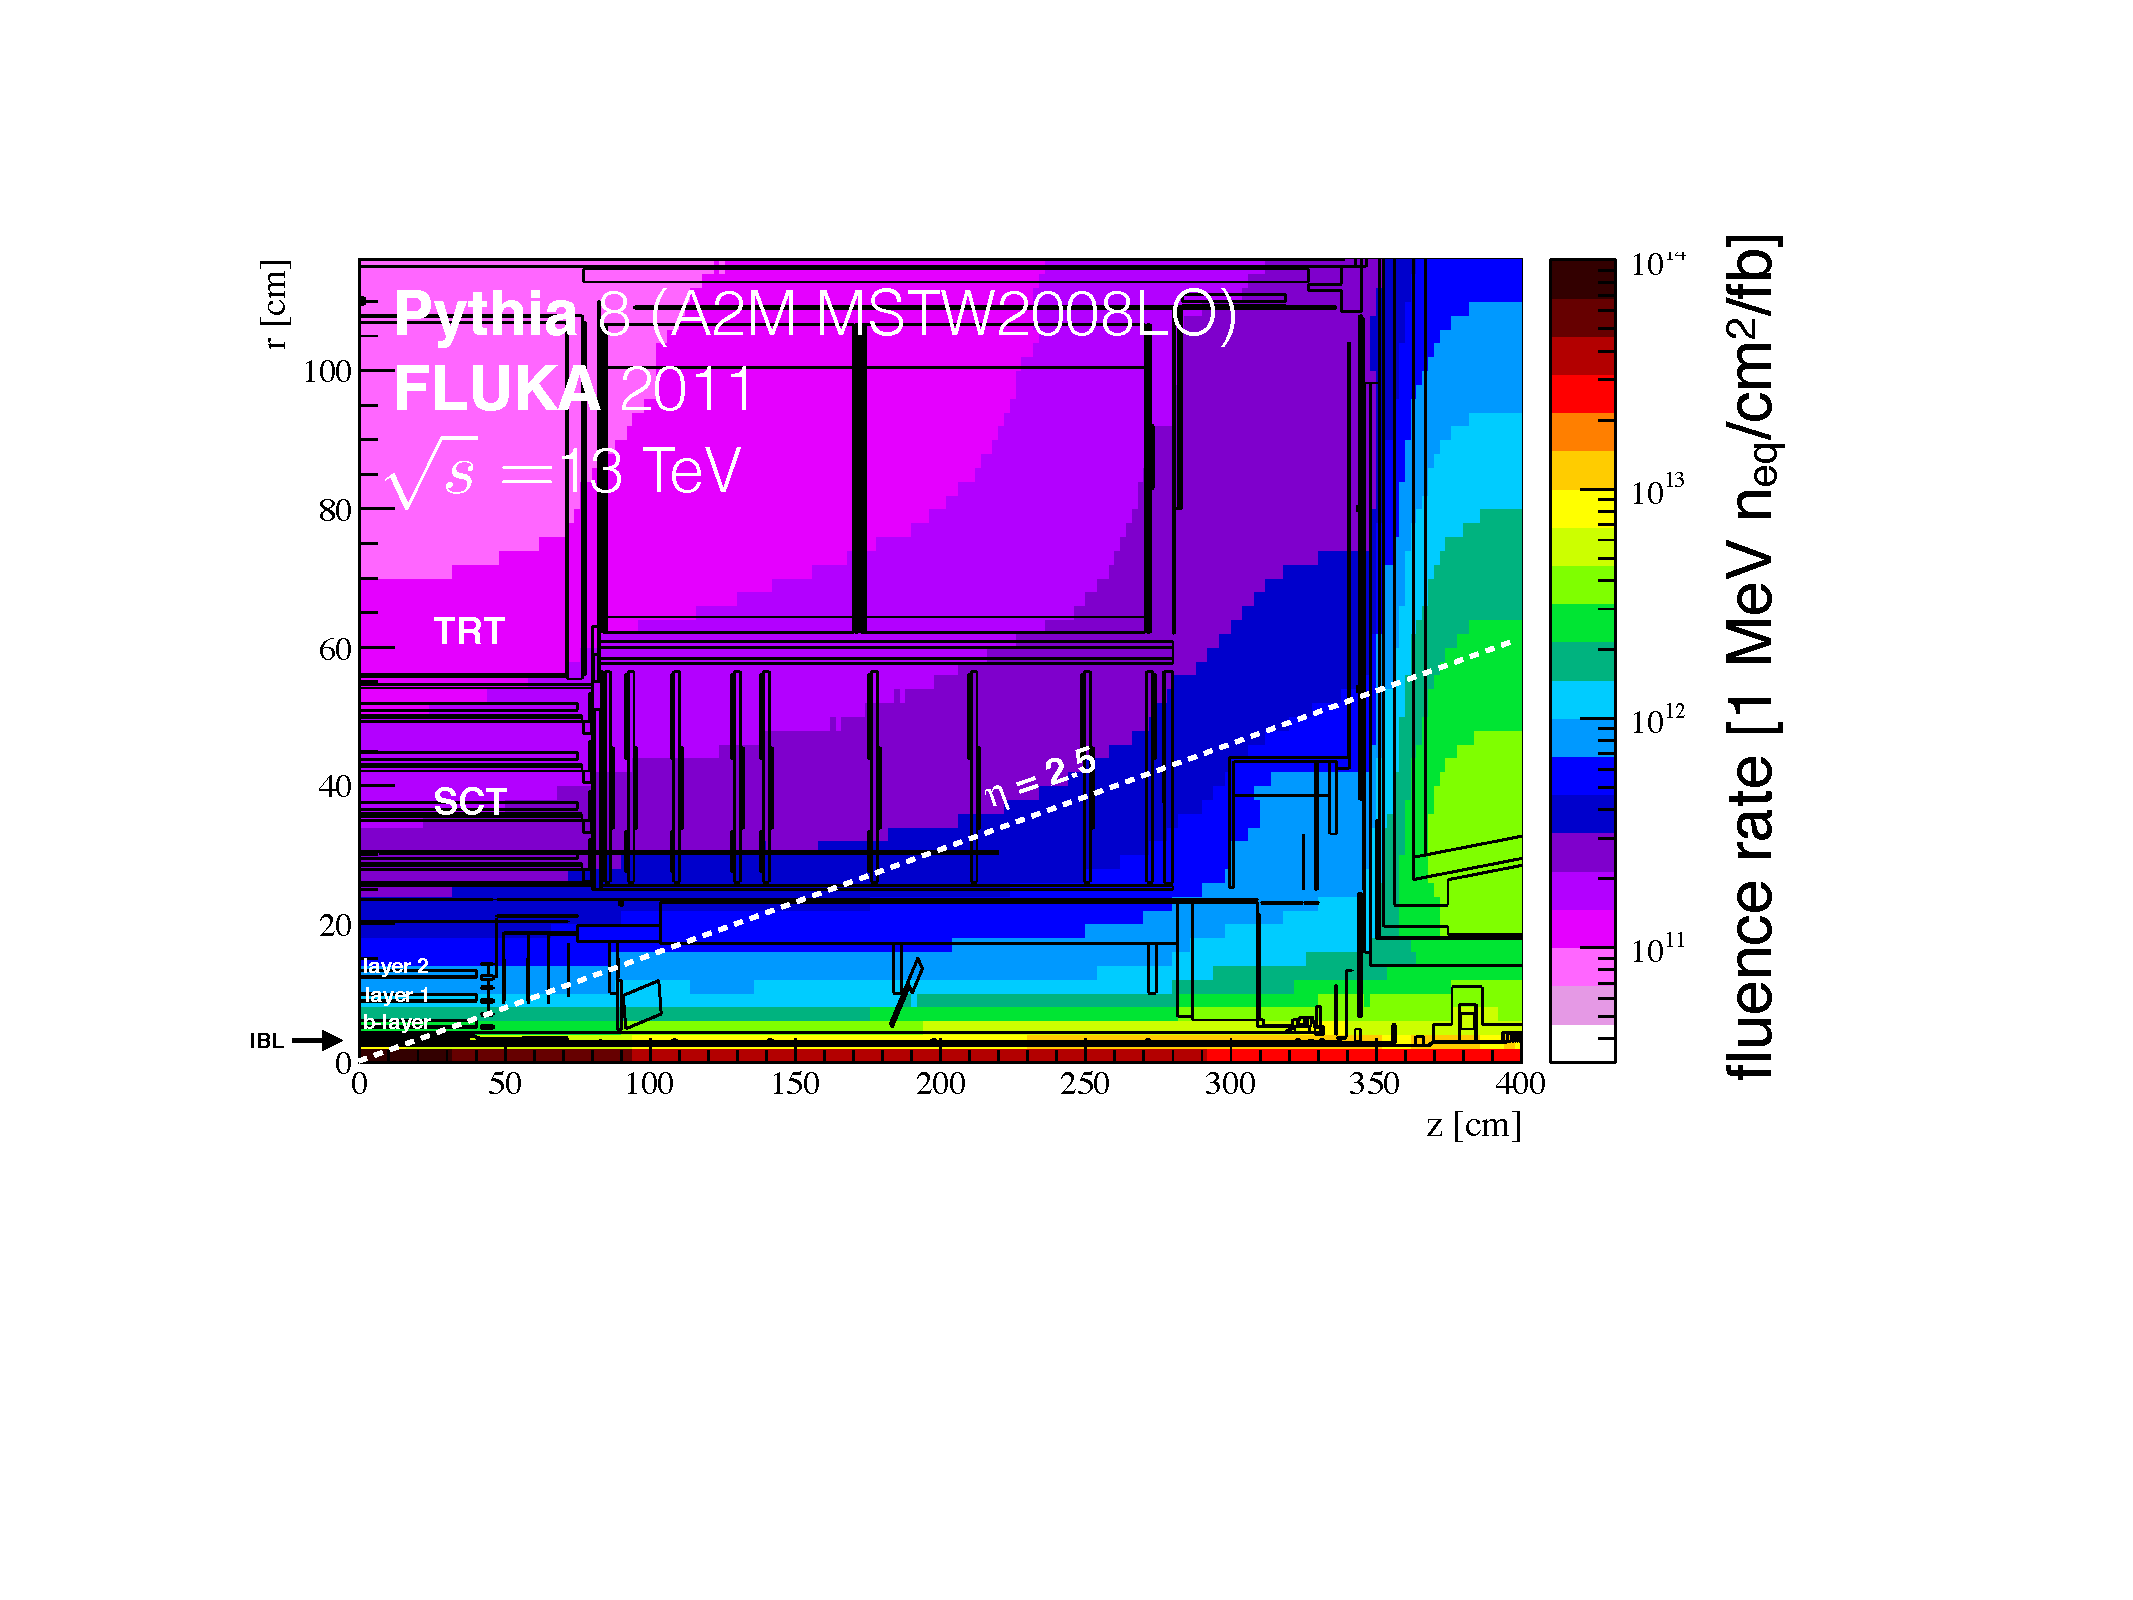
\includegraphics[width=0.6\textwidth]{Labeled2.pdf}
\caption{Simulated 1 MeV $n_\text{eq}$ fluence predictions shown as a function of the radial and longitudinal distance from the geometric center of the detector for a one-quarter slice through the ATLAS FLUKA geometry. Modeled are the pixel, SCT and TRT detector systems and services, and beyond $z = 350$ cm the end-cap calorimeter can be identified.}
\label{fig:fluenceoverview2}
\end{figure}

\begin{figure}[htpb!]
\centering
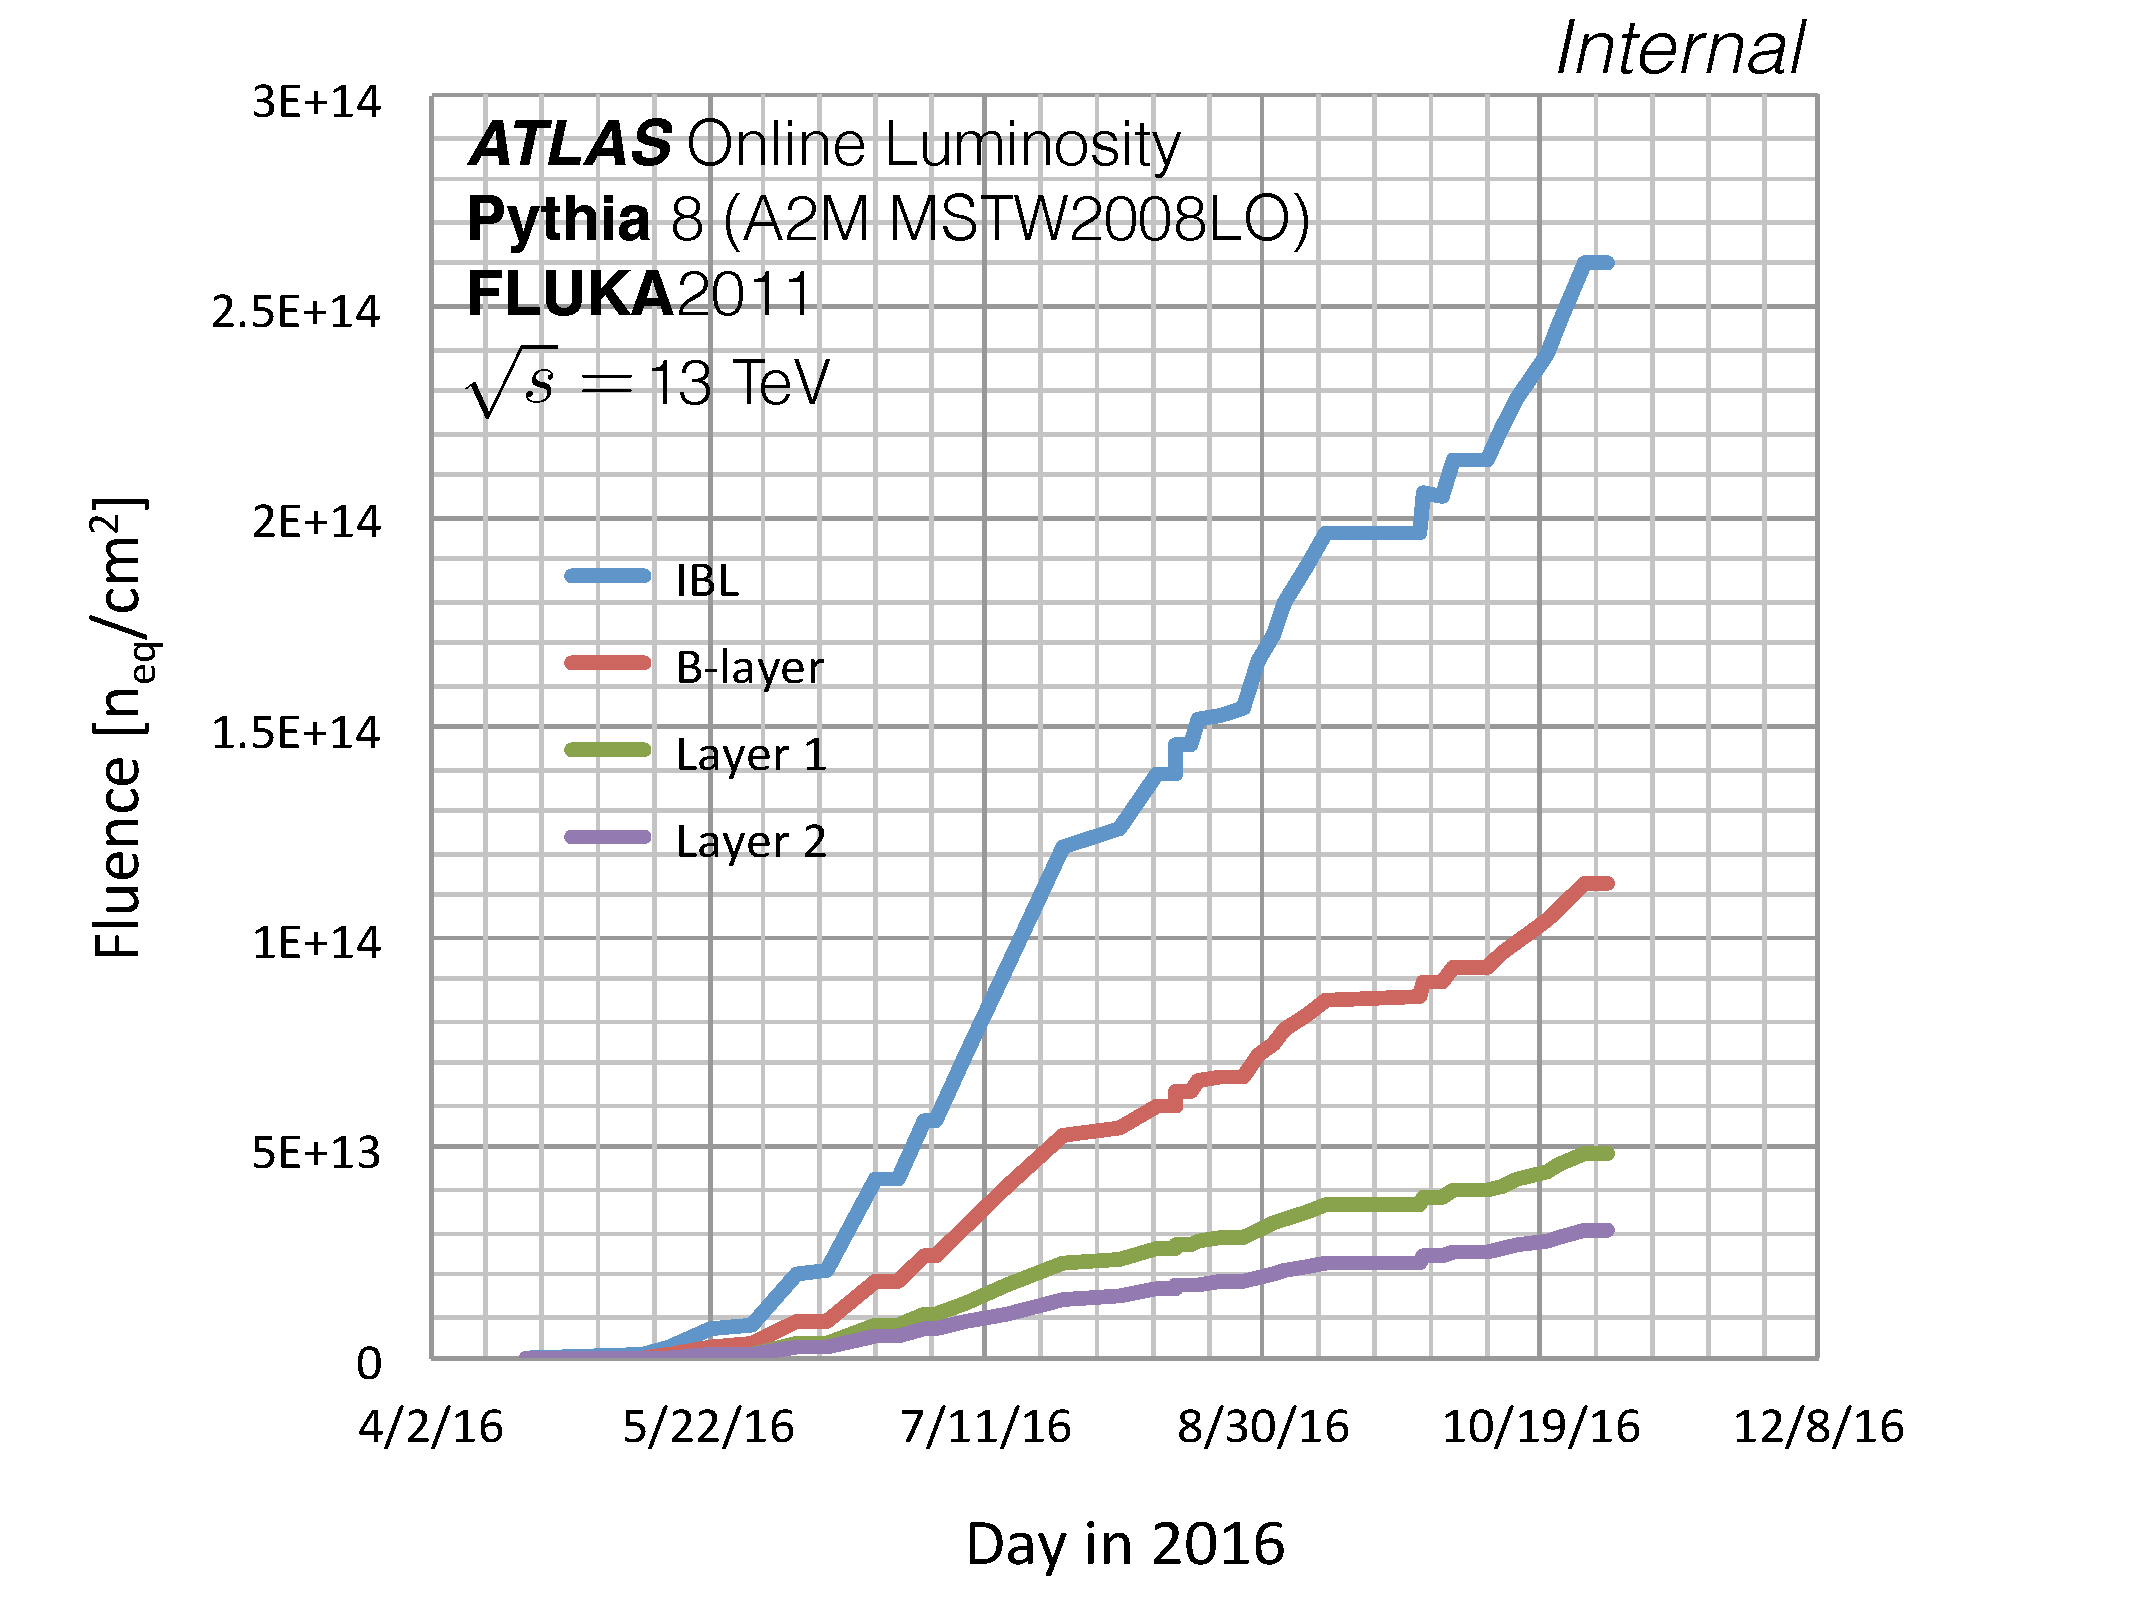
\includegraphics[width=0.49\textwidth]{Fluence_2016}
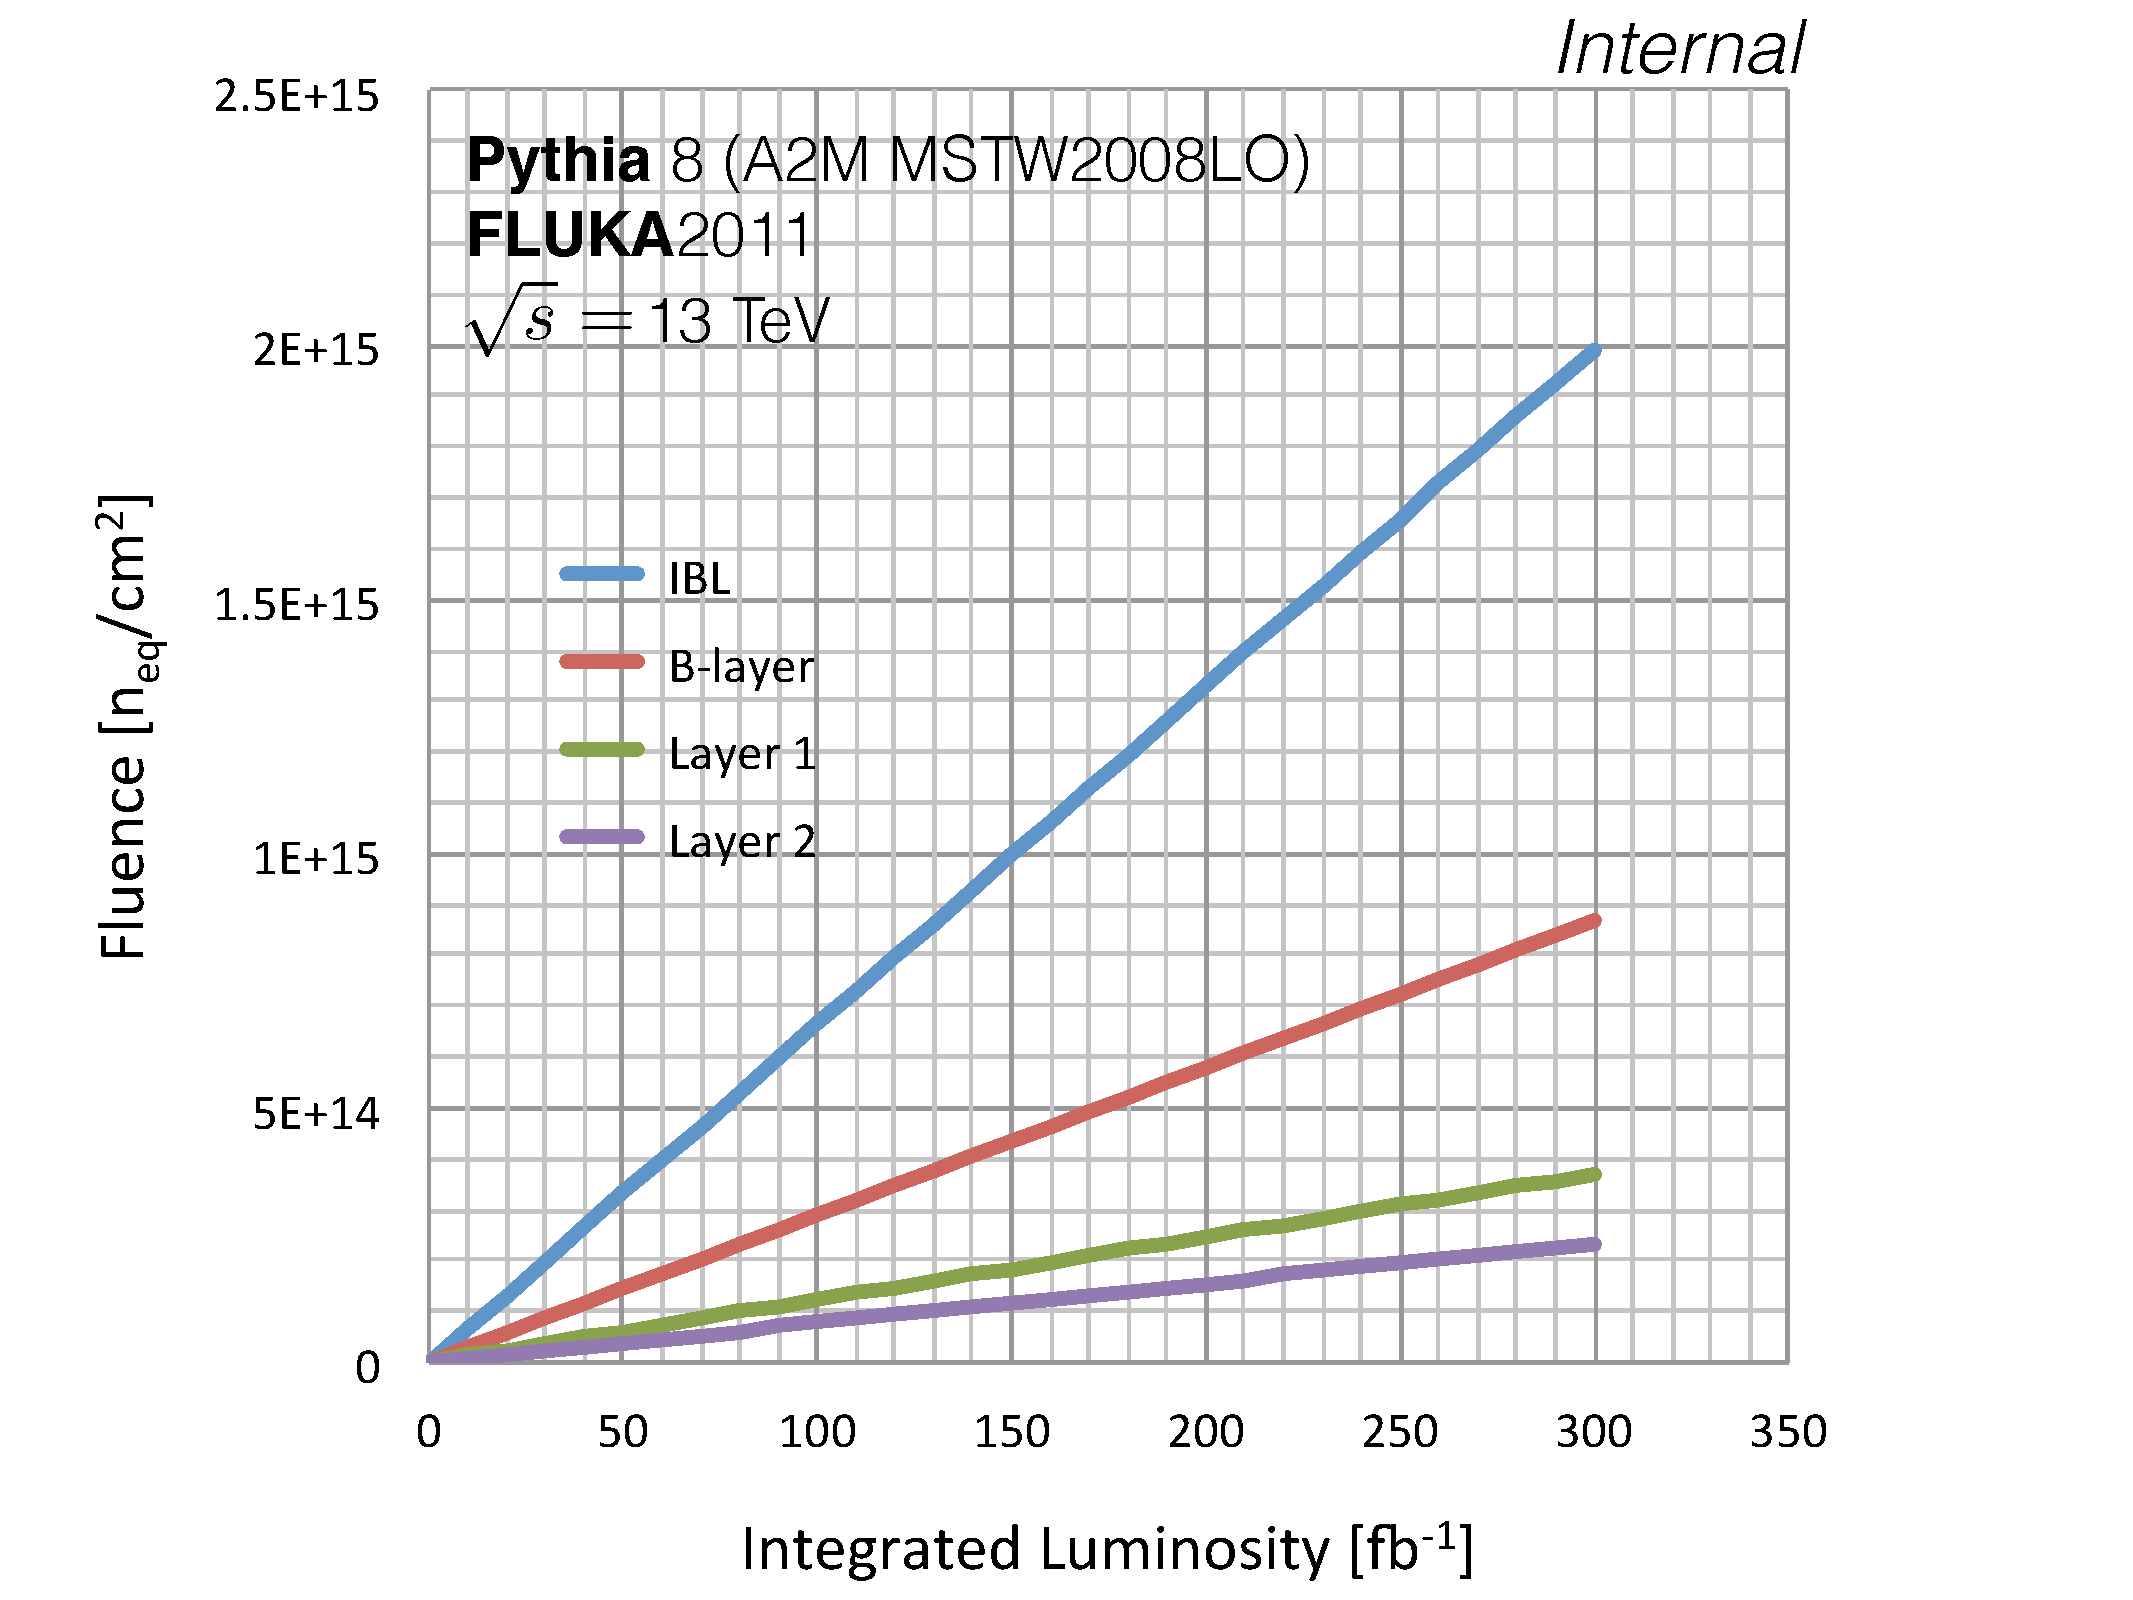
\includegraphics[width=0.46\textwidth]{Fluence_Run23.pdf}
\caption{Predictions for the fluence experienced by the four layers of the current ATLAS Pixel detector during Runs 2 and 3 of the LHC at $|\eta|\approx 0$.  The left plot shows the fluence accumulated during the 2016 run as a function of time while the right plot shows the fluences expected over all of Runs 2 and 3 as a function of integrated luminosity.}
\label{fig:fluenceoverview}
\end{figure}
  



The CMS collaboration has developed a model of radiation damage~\cite{Contardo:2020886,Swartz2002,Chiochia:2004qh,Swartz:2005vp}, validated with testbeam data, but is used to apply corrections to simulation from a model without inherent radiation damage effects.  The next section describes the physics of the digitization model and the first collision data comparisons are shown in Section~\ref{sec:digivalidation}.


\section{Full Digitizer Model}
\label{sec:fullmodel}

\subsection{Overview}

Figure~\ref{fig:app:raddamge1} presents a schematic overview of the physics models included in the digitization model.   
\begin{figure}[htpb!]
\centering
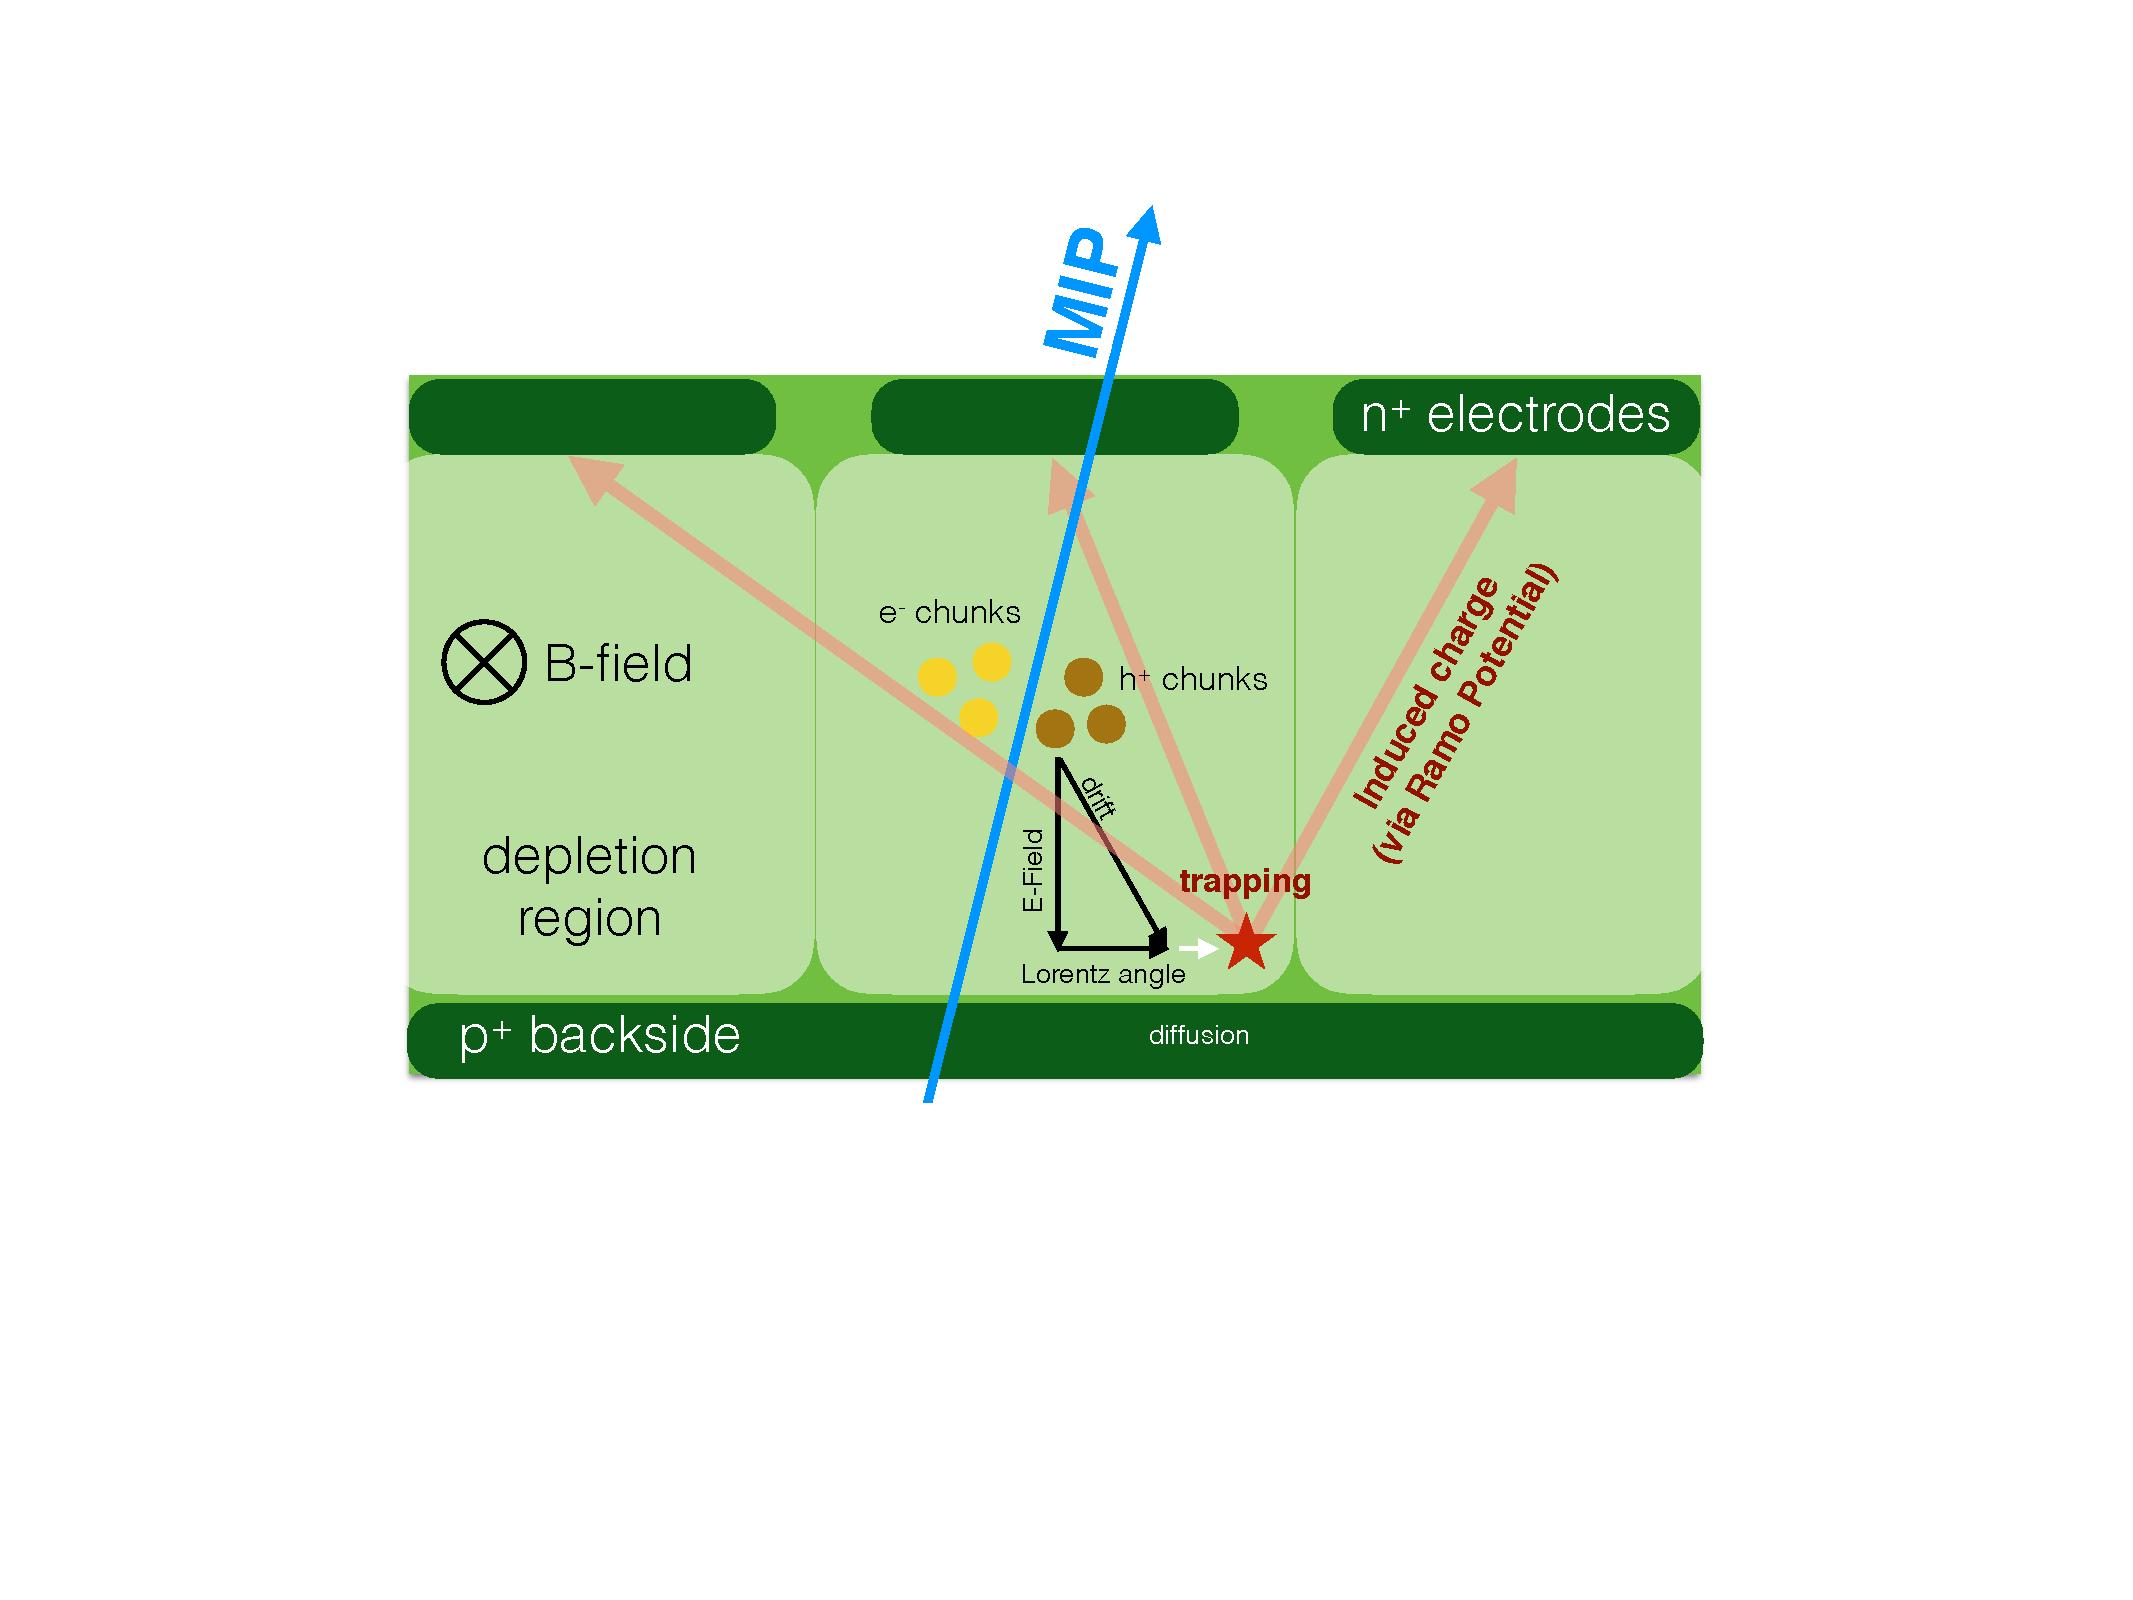
\includegraphics[width=0.95\textwidth]{DigitizerSchematic}
\caption{A schematic diagram illustrating the components of the digitizer model described in this note.  The blue line represents a minimum ionizing particle traversing the pixel sensor.  Chunks of electrons and holes, each representing $\mathcal{O}(10)$ fundamental charges, are transported to the electrodes.  Holes drift toward the backplane under the influence of the electric field and also experience transverse motion due to the magnetic field (deflecting at the Lorentz angle).  Thermal diffusion also changes the position of the charges.  Before being collected, electrons or holes may be trapped by defects in the silicon.  Even though the charge chunk may be trapped, it still induces a charge on the primary and neighbor electrodes via the Ramo potential.  }
\label{fig:app:raddamge1}
\end{figure}

Digitiser inputs are:
\begin{itemize}

\item the detector geometry and conditions, including the fluence (Section~\ref{sec:fluence});
\item the  energy deposition from a charged particle, produced by Geant4~\cite{Agostinelli:2002hh}, possibly with corrections for straggling in thin silicon~\cite{Bichsel:1988if};
\item the electric field, including radiation damage effects (Section~\ref{sec:ElectricField:SimulationDetails}); TCAD simulations are used to model the electric field.
 \end{itemize}
 
 An appropriate bias voltage is determined to ensure a large depletion region (Section~\ref{sec:depletionvoltage}).  Ionisation energy is converted into electron-hole pairs ($\sim 3.6$ eV/pair) which experience random motion from diffusion.  Chunks of fundamental charge carriers drift toward the electrode (electrons) or backplane (holes) under the influence of the electric field, with a field- and temperature-dependent mobility.  The number of fundamental charges per chunk is tuned to save time and a correction is applied to account for an over-estimation of fluctuations (Section~\ref{sec:chunking}).  In addition to drifting toward the electrodes under the influence of the electric field, there is a transverse component to the drift due to the 2 T magnetic field in the ATLAS inner detector.  A field- and temperature-dependent Lorentz angle is combined with the mobility to compute the time for a charge carrier to be collected (Section~\ref{sec:maps},\ref{sec:mapsLorentz}).  This time is compared to a fluence-dependent trapping time (Section~\ref{sec:chargetrapping}), the characteristic time a charge carrier will travel for before it is trapped.  If the drift time is longer than the trapping time, the chunk is declared trapped.  The location of the chunk at the trapped position is calculated based on the starting position and trapping time (Section~\ref{sec:maps}).  Since moving charges induce a current in the collecting electrode, signal is induced on electrodes from trapped charges as well.  This induced charge also applies to neighboring pixels, which contributes to charge sharing.  The induced charge from trapped chunks is calculated from the initial and trapped positions using a weighting potential (Section~\ref{sec:ramo}).  The sum of the collected and induced charge is then converted into a ToT that is used by cluster and track reconstruction tools.



\subsection{Luminosity to Fluence}
\label{sec:fluence}



 The most important input to the radiation damage digitizer is the estimated NIEL.  
 Section~\ref{sec:expflu} introduced the baseline FLUKA simulation that is used to determine the 
 conversion factor between integrated luminosity and fluence. This prediction yields a conversion of
  about $59.6\times 10^{11}$ $n_\text{eq}/\text{cm}^2/\text{fb}^{-1}$ for the IBL and $29.2\times 10^{11}$ $n_\text{eq}/\text{cm}^2/\text{fb}^{-1}$ for the $b$-layer. In order to establish systematic uncertainties on these predictions, the fluence is converted into a prediction for the leakage current. The leakage 
current can be precisely measured and therefore provides a powerful constraint on the FLUKA simulation. For a time $t$ at constant temperature $T$ after an instantaneous irradiation with fluence $\Phi$, the predicted leakage current is given by Equation~\ref{eq:alpha_annealing} already presented 
in~Section\ref{sec:RadDam}.

The full leakage current is then estimated by discretizing time into four hour periods, averaging luminosity and temperature information if finer in a particular period, and then sum over time in Eq.~\ref{eq:alpha_annealing}.  This leads to a complication in the $\alpha_0$ parameter that has no explicit time dependence, but does depend on temperature.  One proposal\footnote{Another proposal is to sum the inverse temperatures~\cite{Barney:1709387}.  Such a method has been compared with Eq.~\ref{eq:leakage2} and results in similar predictions for the leakage current with the current fluence levels and annealing times.}~\cite{moll-thesis} is to absorb the temperature dependence in Eq.~\ref{eq:alpha_annealing} into the logarithm term as an effective scaling of the time axis:

\begin{align}
\label{eq:leakage2}
I_\text{leak}=V\cdot\Phi\cdot\left(\alpha_Ie^{-t/\tau}+\alpha_0^*-\beta\log(\Theta(T)t/t_0)\right),
\end{align}

\noindent where $\alpha_0^*=7.07\cdot 10^{-17}\;$A/cm is the value of $\alpha_0$ from Eq.~\ref{eq:alpha_annealing} evaluated at a reference temperature $T_\text{ref}=21^{\circ}$C and the time scaling function $\Theta(T)$ is defined by

\begin{align}
\label{eq:tempscaling}
\Theta(T) = \exp \left[ - \frac{E_I^*}{k_\text{B} } \left( \frac{1}{T} - \frac{1}{T_\text{ref} } \right) \right],
\end{align}

where $E_I^*=(1.3\pm 0.14)$ eV.  For a fixed time period with constant temperature, Eq.~\ref{eq:alpha_annealing} and Eq.~\ref{eq:leakage2} are mathematically identical.  However, the latter allows for a natural extension to non-constant temperature:

\begin{align}
\label{eq:leakage_modified}
I_\text{leak}=V\cdot\sum_{i=1}^n\cdot\phi_i\cdot t_i\cdot\left[\alpha_I\exp\left(-\sum_{j=i}^n\frac{t_j}{\tau(T_j)}\right)+\alpha_0^*-\beta\log\left(\sum_{j=i}^n\frac{\Theta(T_j)\cdot t_j }{ t_0}\right)\right],
\end{align}

where $\phi_i$ is the fluence rate, $t_i$ is the time in period $i$, and $T_i$ is the temperature in period $i$.  The first sum is over all time periods and the two sums inside the exponential and logarithm functions are over the time between the irradiation in time period $i$ and the present time.

Using the measured module temperature as a function of time, Eq.~\ref{eq:leakage_modified} is used to predict the leakage current as shown in Fig.~\ref{fig:leackagecurrent:beta}. Module properties were updated every ten minutes.  Since the IBL was newly inserted before the 2015 run, it is expected that the leakage current starts off at zero.  A constant luminosity-to-fluence conversion factor is fit to the data per module group in the dashed region near the end of the run.  Module groups differ by their distance along the beam direction from the geometric center of the detector.  The fitted prediction provides an excellent description of the data over the entire Run for all four module groups considered in Fig.~\ref{fig:leackagecurrent:beta}.  There is a clear $z$-dependence on the observed spectrum which is compared with the FLUKA predictions described in Section~\ref{sec:expflu} in Fig.~\ref{fig:leackagecurrent:eta}.  The predictions match the measured values well at $z=0$ with some deviations observed at higher $z$.  The remainder of this Section focuses on central $z$, using the FLUKA simulations without modification for the central value, but with a $15\%$ uncertainty on the fluence.  The ATLAS tracking acceptance is $|\eta|<2.5$, which corresponds to $z\approx 20$ cm in the IBL.

\begin{figure}[!htpb]
\centering
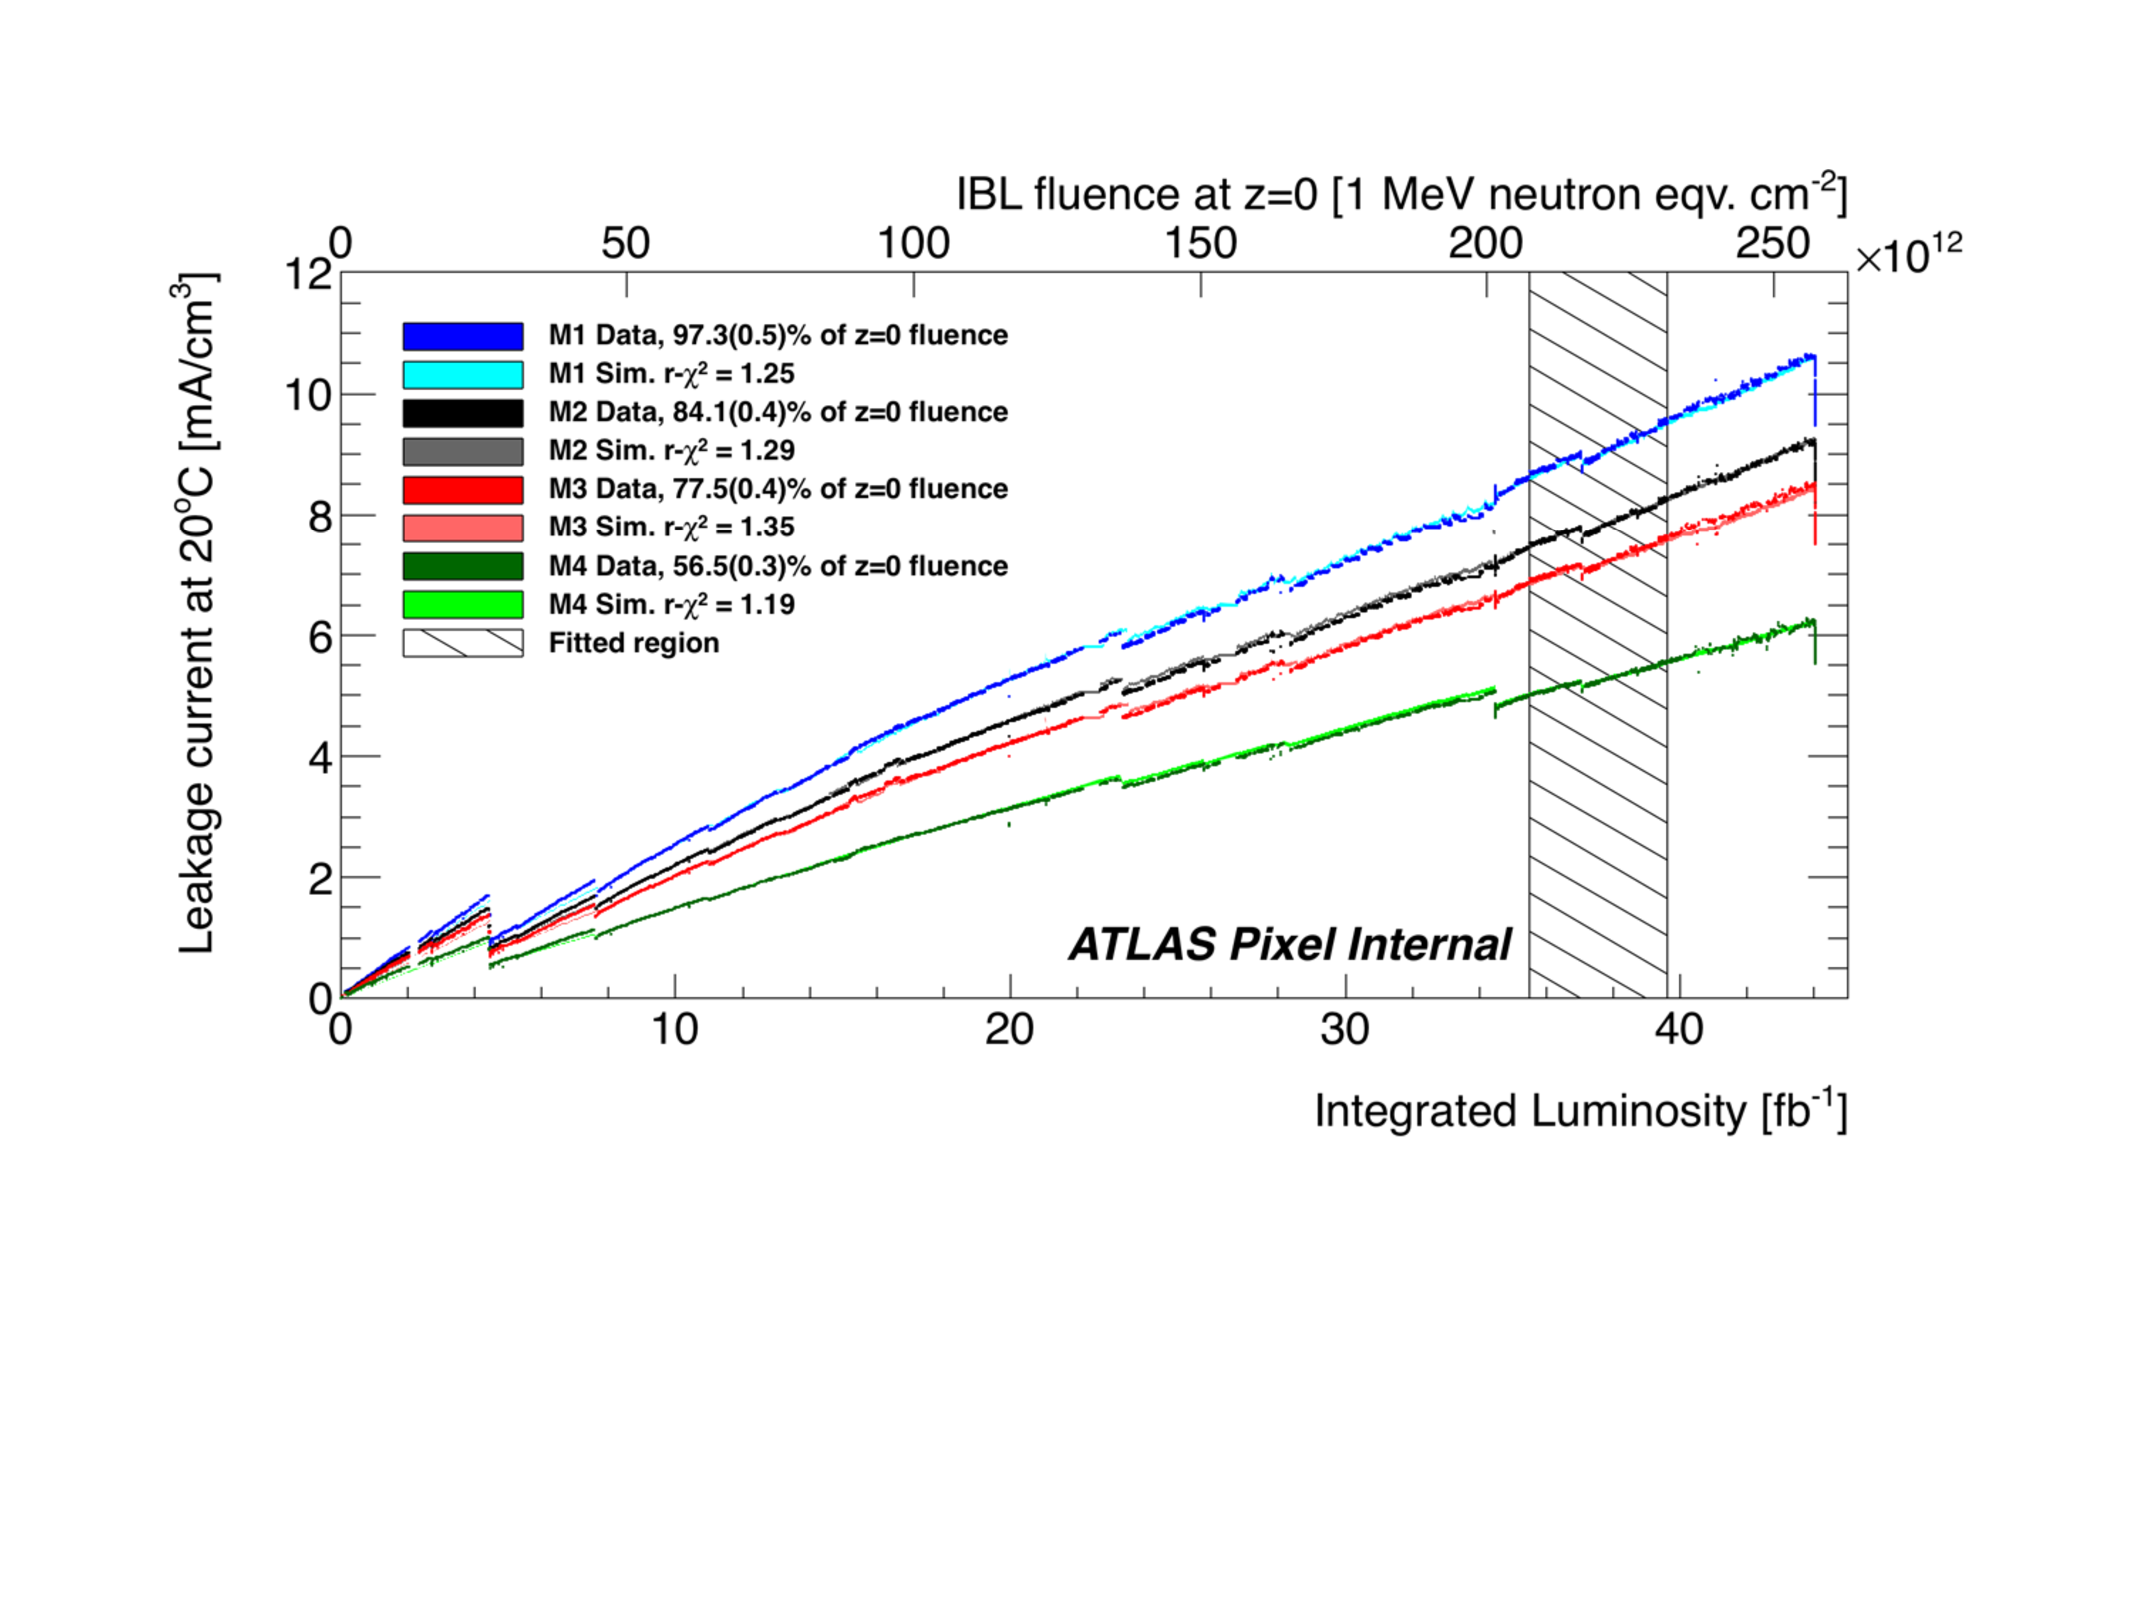
\includegraphics[width=0.85\textwidth]{leakagecurrent_Dann.pdf}
\caption{The measured and predicted leakage current for the IBL as a function of date since the start of the 2015 data run, based on Eq.~\ref{eq:leakage_modified}.   Current spikes and the first and last 200 luminosity blocks of each run are excluded. The leakage current is normalized to a temperature of $20^{\circ}$C. The dashed region indicates the normalization region for the fit for the luminosity-to-fluence conversion factor per module group. Each module group is $8$ cm long on each side of the detector along the beam direction.  The groups M1, M2, M3 approximately span the ranges $z\in[-8,8]$ cm, $|z|\in[8,16]$ cm, and $|z|\in [16,24]$ cm, respectively. }
\label{fig:leackagecurrent:beta}
\end{figure}

\begin{figure}[!htpb]
\centering
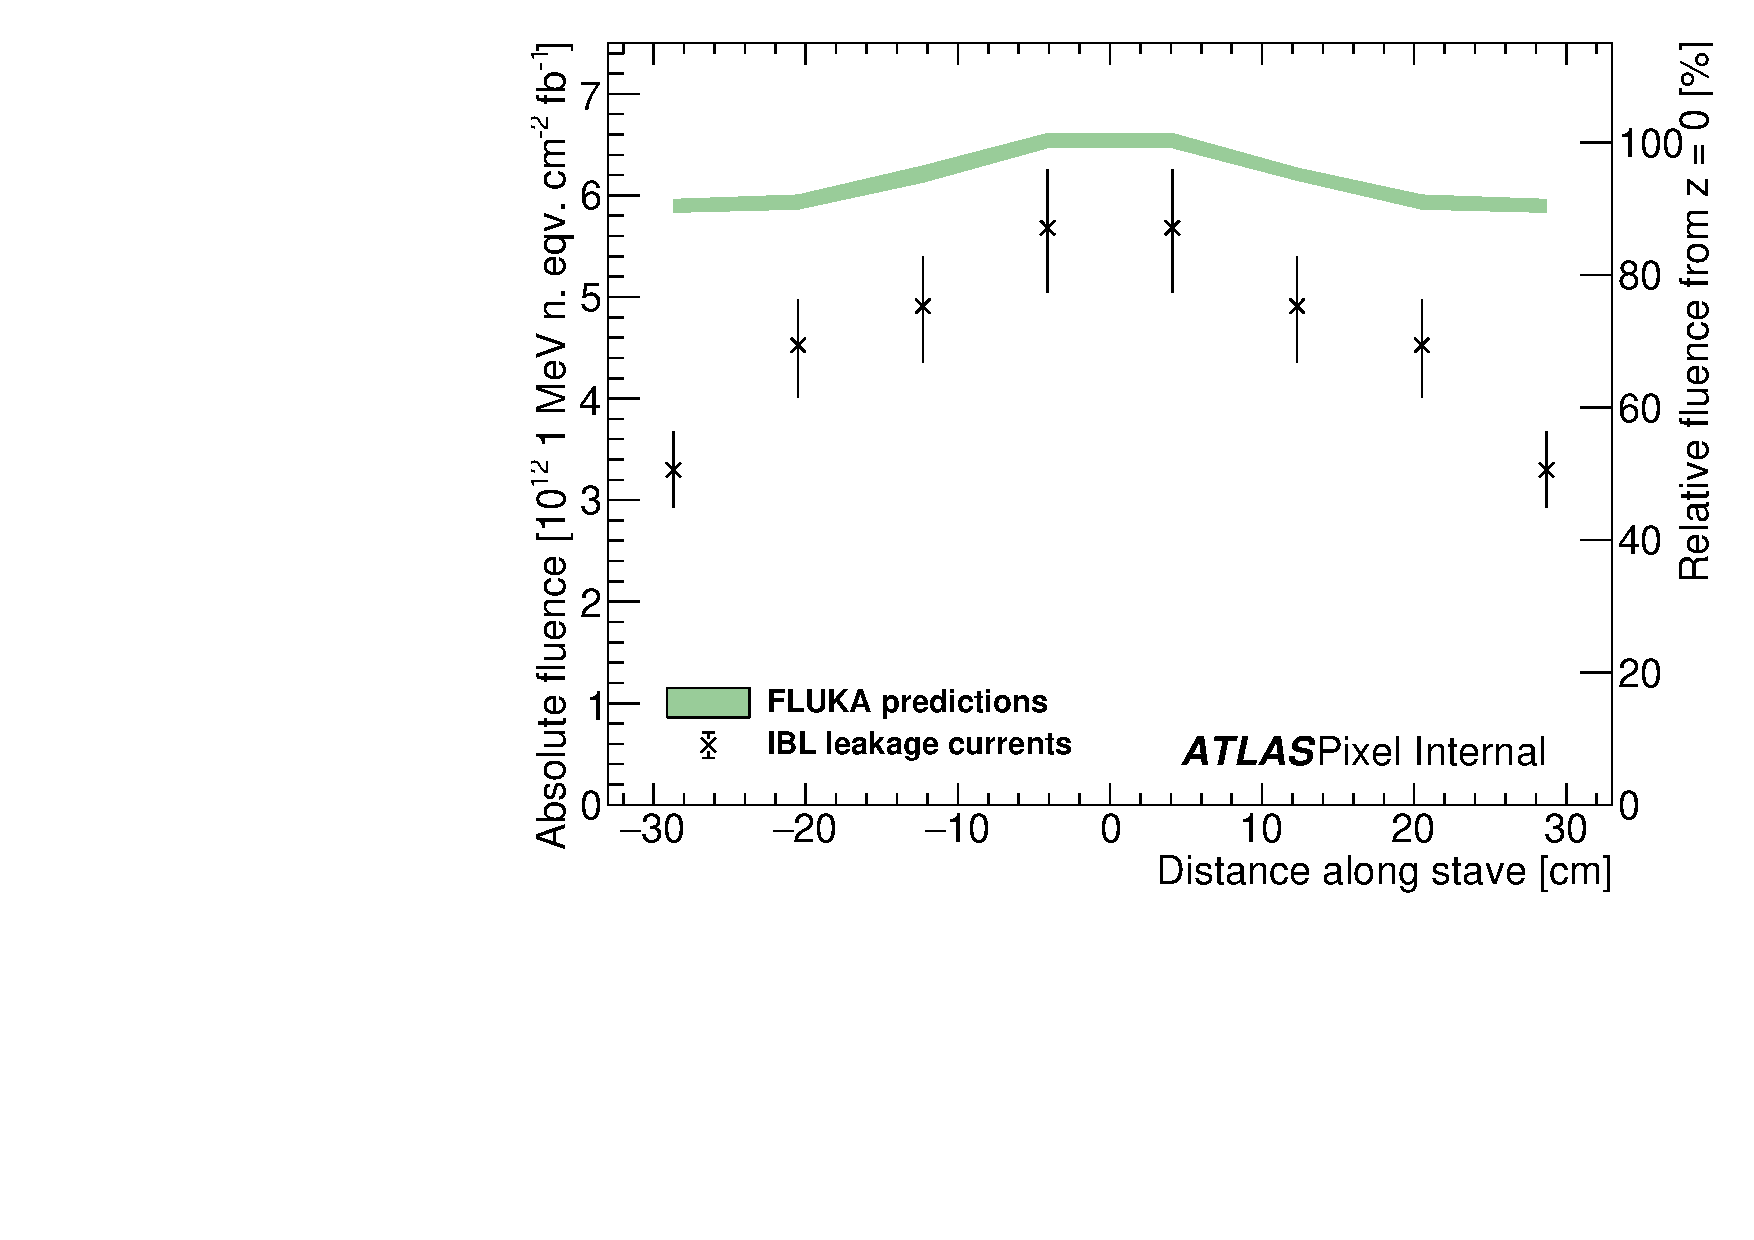
\includegraphics[width=0.65\textwidth]{simulation-FLUKA-absolute.pdf}
\caption{The fluence-per-luminosity conversion factors extracted from leakage current fits as a function of z, compared with the FLUKA predictions described in Section~\ref{sec:expflu}. The leakage current error bars are dominated by a conservative $10\%$ uncertainty, accounting for the variation in the bias voltage at full depletion~\cite{ATL-INDET-PUB-2014-006}.  Uncertainties due to the annealing model ($0.1\%$) and data fit ($0.5\%$) are subdominant.}
\label{fig:leackagecurrent:eta}
\end{figure}

\subsection{Electric Field Modelization}
The radiation-induced states in the silicon band gap affect the electric field in the pixel cells by altering 
the electric field distribution in the bulk\footnote{There are also changes at the surface, but the focus 
here is on the deformations on the electric field within the sensor.}. Since many variables used in signal 
formation calculations depend on the electric field (drifting time, Lorentz angle deviation, etc.), including 
radiation damage effects requires a careful parameterisation of the electric field in the pixels. 
Investigation of the electric field profile in the bulk of irradiated silicon sensors have shown that for 
certain materials, the electric field is no longer linear with the bulk depth after irradiation.  

Section~\ref{sec:ElectricField:SimulationDetails} introduces the default model used for subsequent studies, as well as provides references to alternative models in the literature.   The fluence-dependent depletion voltage calculation is presented in Section~\ref{sec:depletionvoltage} and the resulting field profiles are shown in Section~\ref{sec:Efieldprofile}.  Section~\ref{sec:Efieldmodelcomparisons} provides a brief comparison between the default model and alternative models.

\subsubsection{Simulation Details}
\label{sec:ElectricField:SimulationDetails}

Since the charge collection is significantly different in planar and 3D sensors due to the different electrodes geometries, two different simulation environments are setup to model each sensor type:

\paragraph{Planar}

Investigation of the electric field profile in the bulk of irradiated silicon sensors have shown that the electric field is no longer linear with the bulk depth after irradiation (see, for example, Ref.~\cite{bib:DP,CHIOCHIA2006}). In these materials, the irradiation causes two junctions, one at the pixel side and one at the opposite side, as first explained by Eremin, Verbitskaya, and Li~(EVL)~\cite{bib:DP}. As electrons and holes drift toward the pixel and opposite side, respectively, the current density becomes non-constant along the bulk, causing variation in carrier distribution. The carriers can get trapped while drifting, which translates into non-uniform space charge region with a linear dependence on the bulk depth; this gives rise to an electric field with two maxima at the two edges of the sensor and a minima somewhere in the middle of the bulk.  Field profiles are discussed in more detail in Section~\ref{sec:Efieldprofile}

This important and striking feature of irradiated planar sensors is simulated using the \textit{Chiochia model}~\cite{CHIOCHIA2006}, already introduced in Section~\ref{sec:TCADRadDamModels}, implemented in the Silvaco TCAD package~\cite{silvaco}.  The simulation is performed over volume that corresponds to a quarter of an ATLAS IBL pixel sensor cell, to take advantage of symmetry.  Figure~\ref{fig:planarsetup} highlights the geometry used in the simulation.   The electric field is computed at $T=-10^{\circ}$C using an effective doping concentration of $1.6\times 10^{12}/\text{cm}^3$ (corresponding to about 50 V depletion for unirradiated sensors) with a resolution of $1$ $\text{$\mu$m}^3$.  The Chiochia model is a double-trap model with one acceptor and one donor trap with activation energies set to $E_c-0.52$ eV and $E_v+0.48$ eV~\cite{bib:DP}, respectively.  Reference~\cite{CHIOCHIA2006} gives suggested values of the concentrations and capture cross-sections.  The capture cross section for the acceptor and donor levels for holes, $\sigma_h^A,\sigma_h^D$ are fixed at $1.65$ ($\times 10^{-15}$ cm$^2$) and the same quantities for electrons ($\sigma_e^{A},\sigma_e^D$) are fixed at $6.60\times 10^{-15}$ cm$^2$.  The acceptor and donor concentrations vary with fluence are interpolated from the values presented in Ref.~\cite{CHIOCHIA2006}.  In particular, the acceptor concentrations are set to $0.35, 0.68$, and $1.36\times 10^{15}/\text{cm$^3$}$ for $1, 2$, and $5\times 10^{14}$ $n_\text{eq}/\text{cm}^2$ and the corresponding donor concentrations for the same fluences are $0.5, 1.0$, and $3.39\times 10^{15}/\text{cm$^3$}$.

\begin{figure}[!htpb]
\centering
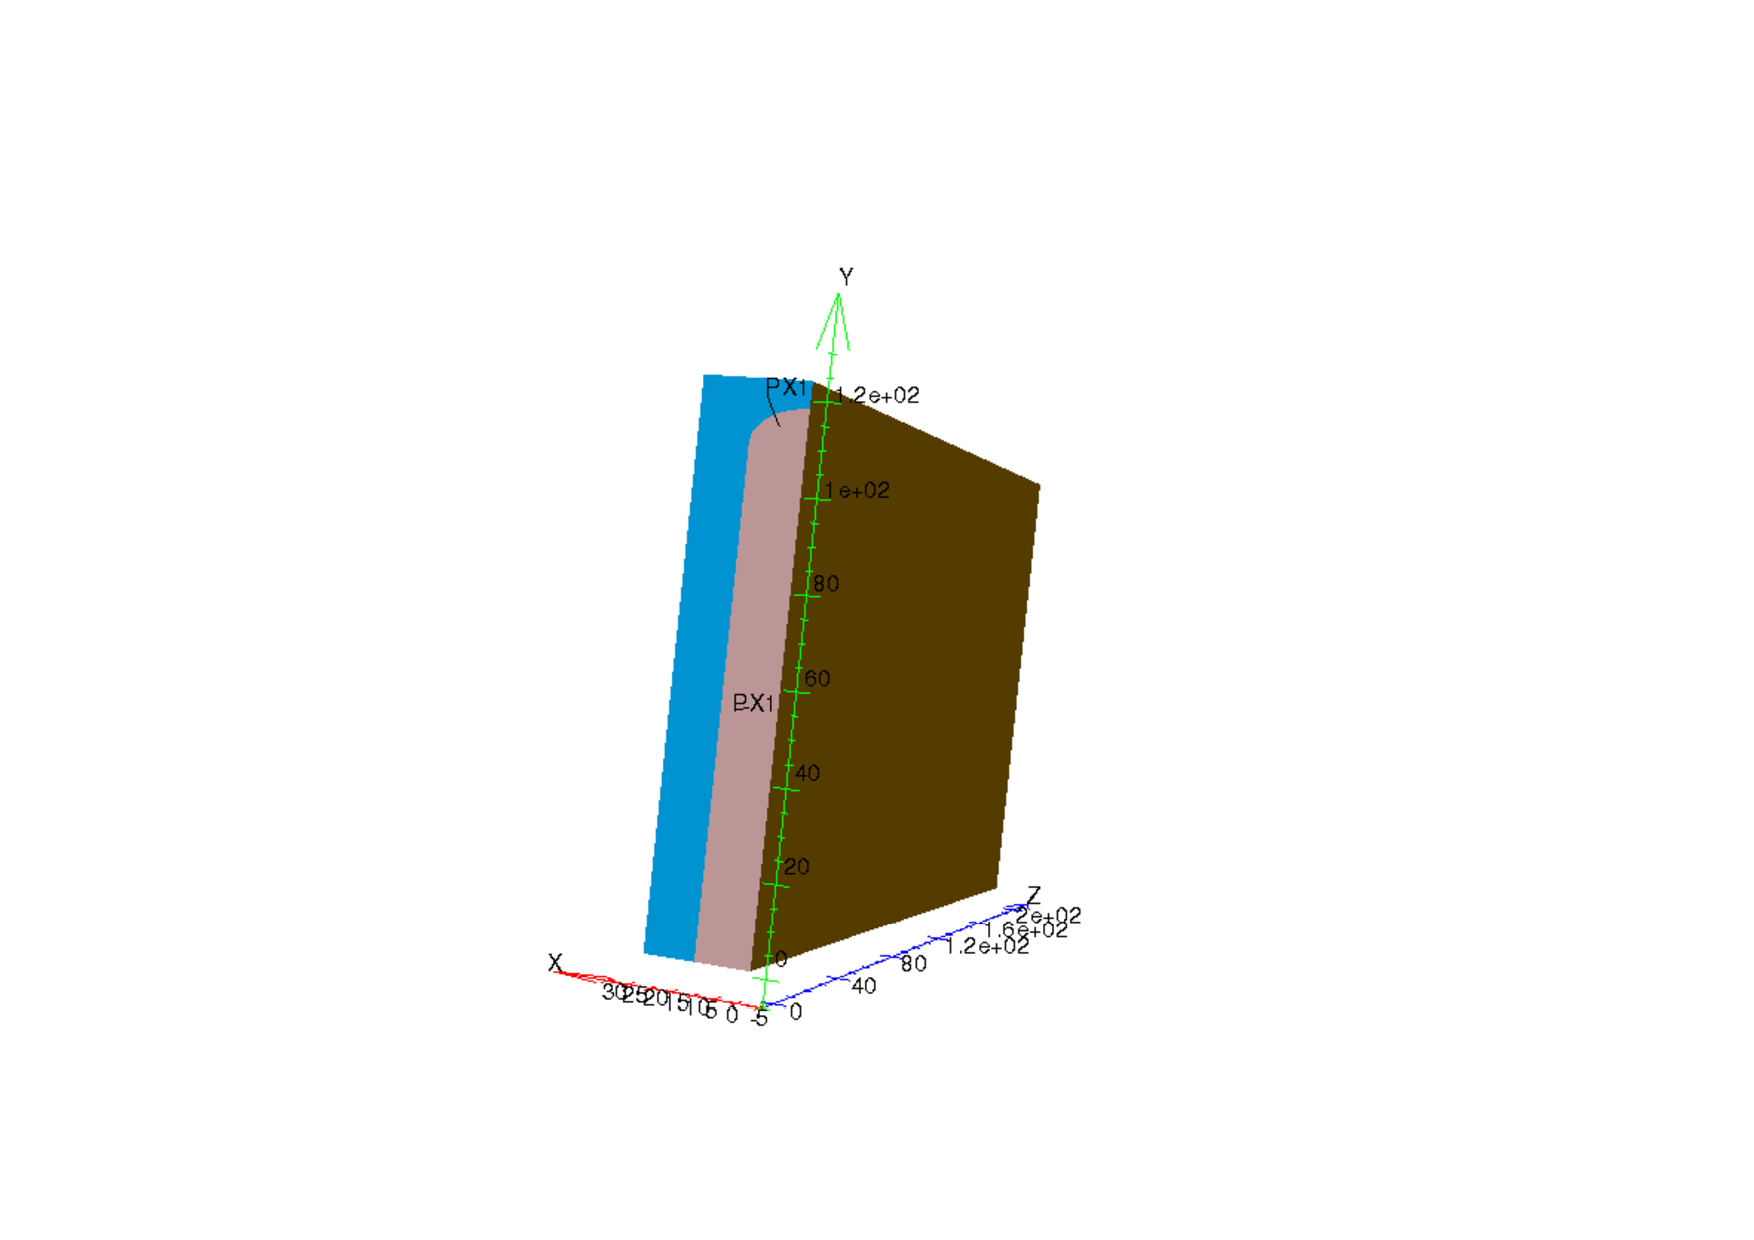
\includegraphics[width=0.3\textwidth]{planar.pdf}
\caption{A schematic setup of the geometry for the planar TCAD simulation.}
\label{fig:planarsetup}
\end{figure}

\paragraph{3D} Radiation damage effects for the 3D sensor are implemented in the \textit{Perugia model}~\cite{7542192} with the Synopsys TCAD package\footnote{\url{https://www.synopsys.com/silicon/tcad.html}}.  As shown in Fig.~\ref{fig:3Dsetup} one-eight of the sensor is simulated to take advantage of the symmetry within the pixel.  In the Perugia model, there are two acceptor and one donor traps, with activation energies given by $E_c-0.42, E_c-0.46$, and $E_v+0.36$, respectively.  The capture cross-sections for electrons for the three levels are $1, 7, 323\times 10^{-15}/\text{cm}^2$ and for holes are $10, 70, 32.3\times 10^{-15}/\text{cm}^2$.  The acceptor and donor concentrations are $1.614\times\Phi,0.9\times\Phi$, and $0.9\times\Phi$, respectively. 

%Definition of introduction rage (IR) is on p57 here: http://www.iaea.org/inis/collection/NCLCollectionStore/_Public/39/025/39025559.pdf.

\begin{figure}[!htpb]
\centering
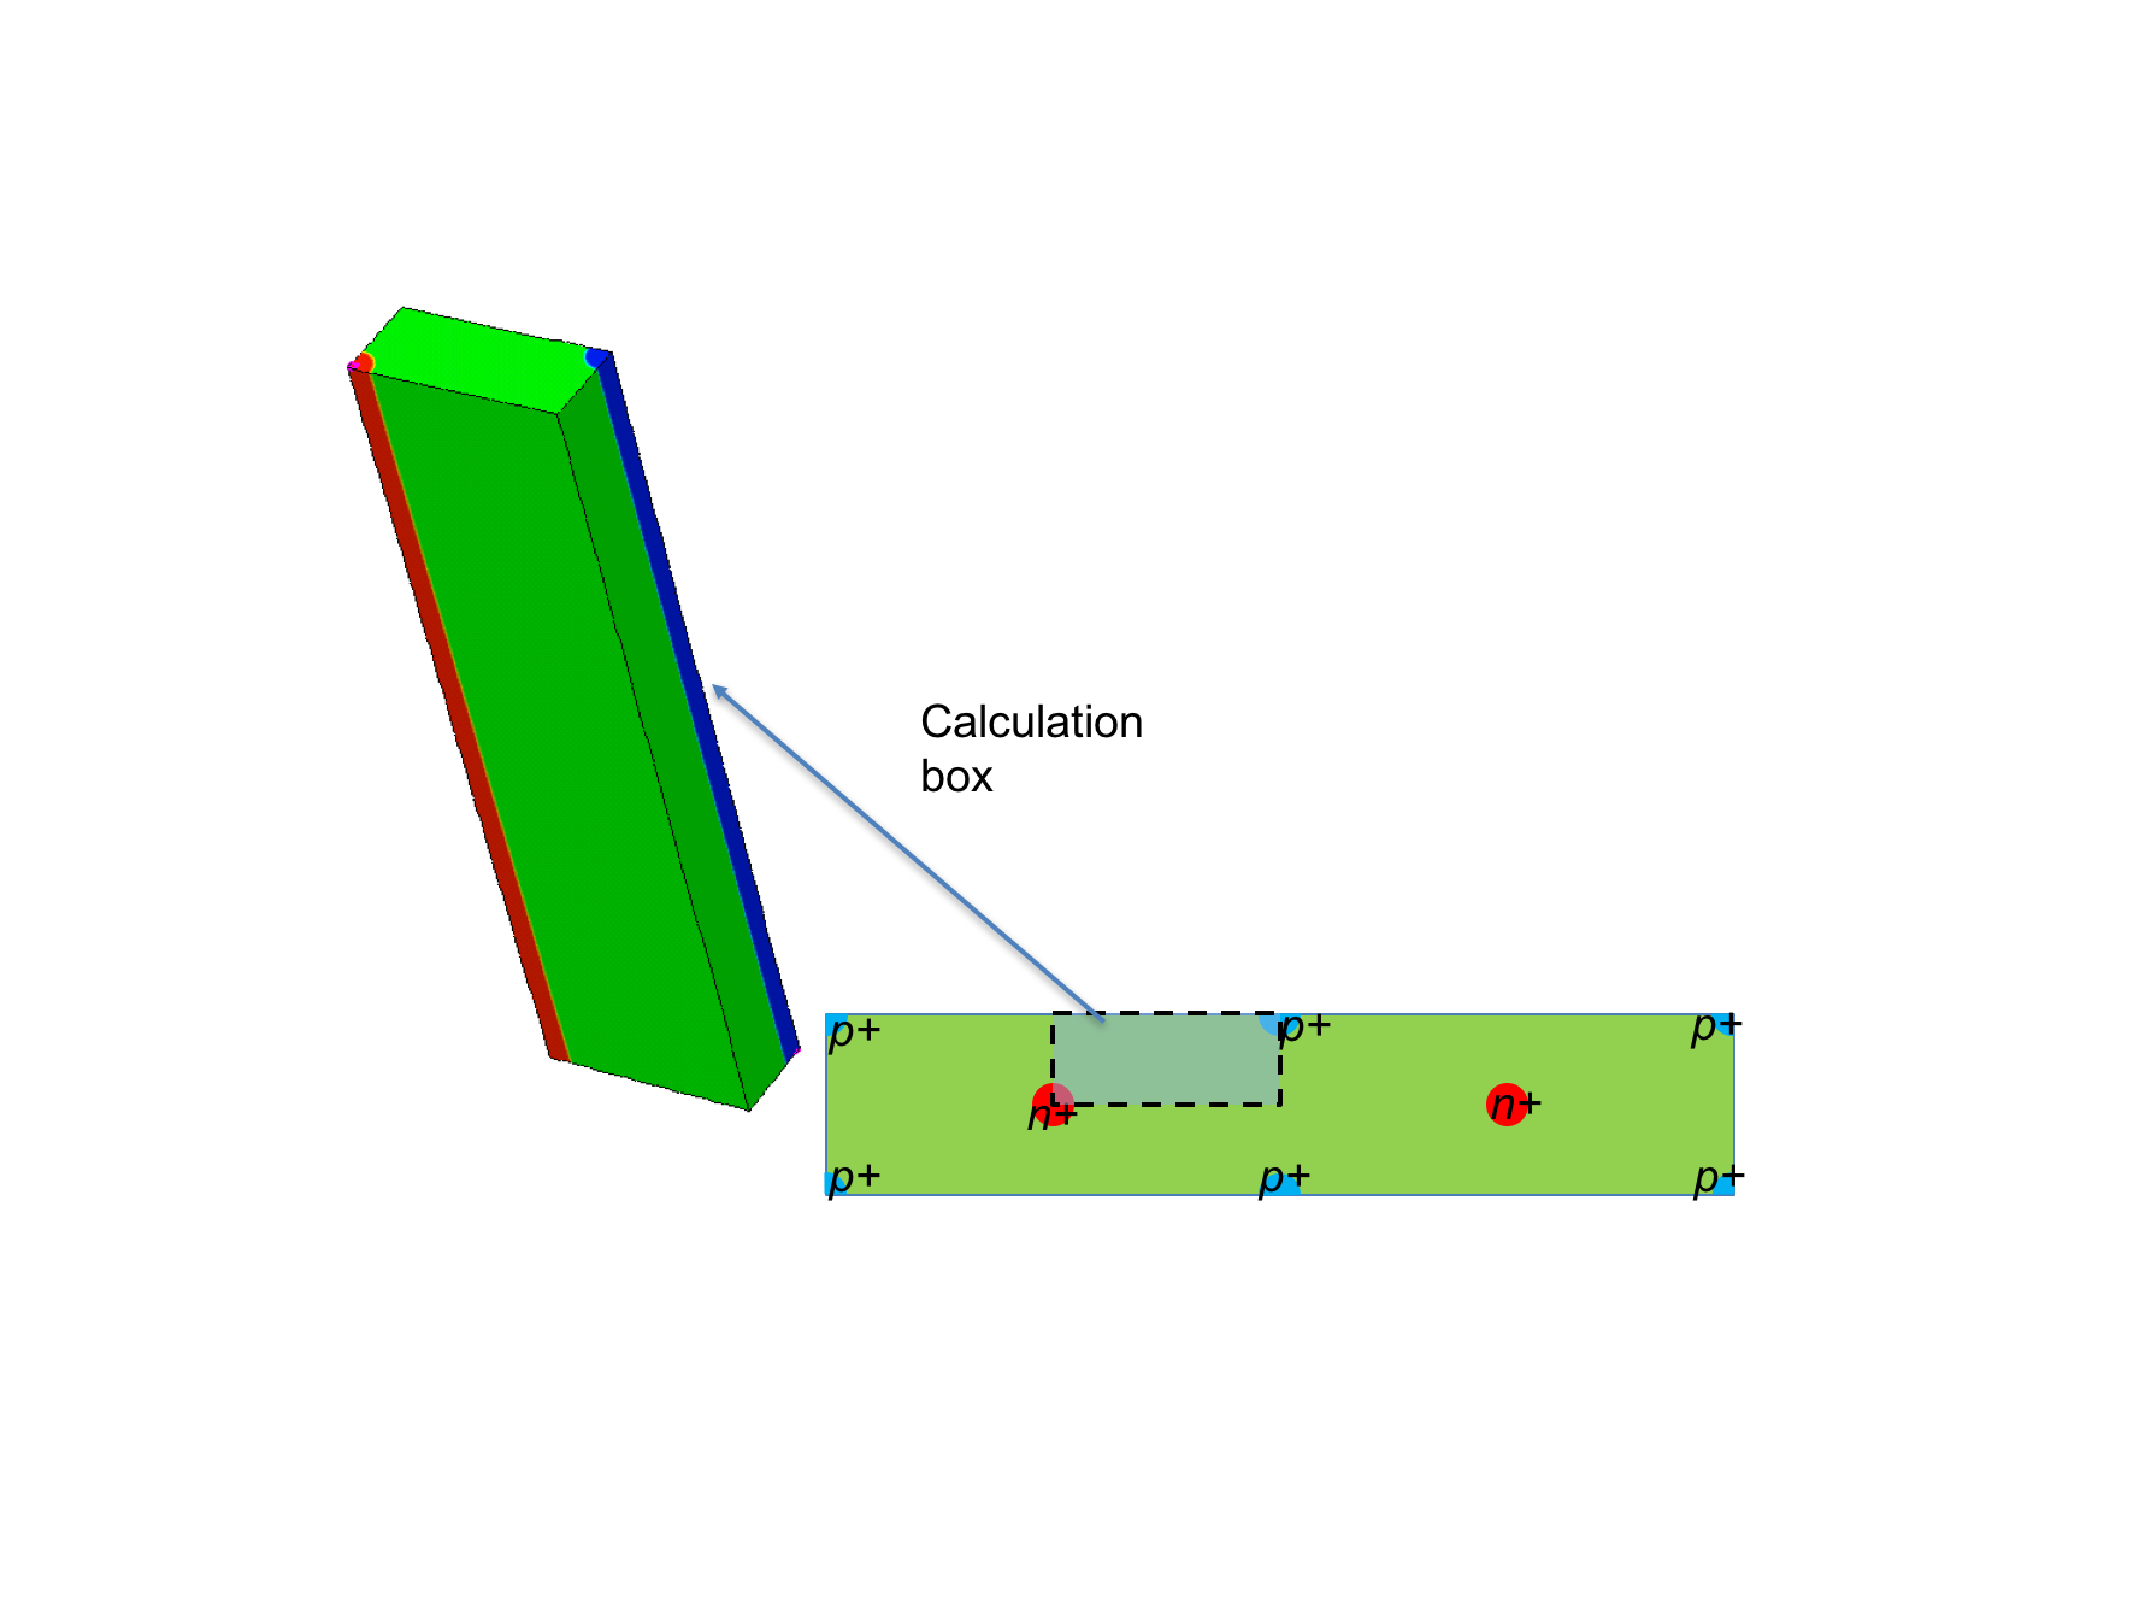
\includegraphics[width=0.5\textwidth]{3D_fig}
\caption{A schematic setup of the geometry for the 3D TCAD simulation.}
\label{fig:3Dsetup}
\end{figure}

While the Chiochia (planar) and Perugia (3D) models are used as default, there are additional radiation damage models (EVL~\cite{bib:DP}, Petasecca~\cite{1710302}, New Delhi~\cite{dalal2014simulation}, etc.), some of which are investigated in Section~\ref{sec:Efieldmodelcomparisons}.  The TCAD simulations for planar and 3D sensors are valid for silicon that has been instantaneously irradiated to a given fluence.   In reality, the irradiation and thermal history play an important role in the effective doping concentration, which influences the calculated electric field profile.  These effects are accounted for with a model of annealing, as described in the next section.


\subsubsection{Annealing}
\label{sec:annealing}

 The irradiation and thermal history are accounted for in the prediction of the effective doping concentration with the Hamburg model (see~\cite{moll-thesis} and references therein).  In this model, the effective doping concentration has the following form:

\begin{align}
\label{eq:hamburg0}
N_\text{eff}(t)=(N_\text{eff}(0)-N_{D}^\text{removable}(0))+N_{D}^\text{removable}(t)-N_{A}^\text{stable}(t)-N_{A}^\text{beneficial}(t)-N_{A}^\text{reverse}(t),
\end{align}

where $N_D^\text{removable}(0)$ is the initial concentration of removable donors.  The fraction of removable donors at low doping concentrations like here is 100\% for charged particle irradiation, which dominates the inner pixel layers in the ATLAS detector.  The time-dependence of the terms on the right-hand side of Eq.~\ref{eq:hamburg0} are described by the following differential equations:

\begin{align}
\label{eq:hamburg1}
&\frac{d }{d t}N_{D}^\text{removable}(t) &&=-c\phi(t) N_{D}^\text{removable}(t)&&\text{removal of donors for $n$-type during irradiation}\\\label{eq:hamburg2}
&\frac{d }{d t}N_{A}^\text{stable}(t) &&= g_c\phi(t)&&\text{introduction of stable defects during irradiation}\\\label{eq:hamburg3}
&\frac{d }{d t}N_{A}^\text{beneficial}(t)  &&=g_A\phi(t)-k_A(T)N_{A}^\text{beneficial}(t) &&\text{beneficial annealing}\\\label{eq:hamburg4}
&\frac{d }{d t}N_{N}^\text{reverse}(t)  &&= g_Y\phi(t)-k_Y(T)N_{A}^\text{reverse}(t) &&\text{reverse annealing - neutrals}\\\label{eq:hamburg5}
&\frac{d }{d t}N_{A}^\text{reverse}(t)  &&= - k_Y(T)N_{N}^\text{reverse}(t) &&\text{reverse annealing - acceptors} 
\end{align}

\noindent where $\phi(t)$ is the irradiation rate in 1 MeV $n_\text{eq}/\text{cm}^2/\text{s}$.  Equation~\ref{eq:hamburg1} represents the effective removal of the initial dopants by mobile defects.  The removal constant is $c=6.4118\times 10^{-14}/\text{cm}^2$.  The second equation, Eq.~\ref{eq:hamburg2} represents the constant addition of stable (non-annealable) defects which electrically act as acceptors.  Two additional defects are introduced in Eq.~\ref{eq:hamburg3} and~\ref{eq:hamburg4}.  These short-lived defects are introduced during irradiation with rates $g_a$ and $g_Y$ and then decay with sufficiently high temperatures.  The temperature-dependence of the decay rates are modeled with an Arrhenius equation, $k_i(T)=k_{i,0}e^{-E_i/k_bT}$, where $k_{A,0}=2.4\times 10^{13}/\text{s}, k_{Y,0}=7.4\times 10^{14}/\text{s}$, $E_A=1.09$ eV and $E_Y=1.325$ eV.  For the beneficial annealing (Eq.~\ref{eq:hamburg3}), the acceptor-like defects introduced during irradiation decay to neutral states with a time constant that is $\mathcal{O}(\text{days})$ at $20^{\circ}$C.  In contrast, for reverse annealing, neutral-like defects are introduced during irradiation (Eq.~\ref{eq:hamburg4}). The neutral defects can decay into acceptor-like states (Eq.~\ref{eq:hamburg5}), decreasing (increasing) the effective doping concentration before (after) space-charge sign inversion.  The timescale for reverse annealing is $\mathcal{O}(\text{weeks})$ at $20^{\circ}$C.  The solutions of the differential equations \ref{eq:hamburg1}-\ref{eq:hamburg5} at constant temperature are:

\begin{align}
\label{eq:hamburg12}
&N_{D}^\text{removable}(t) &&=N_\text{c,0}\cdot \left( 1-e^{-c\phi_\text{eq}t} \right) \\ \label{eq:hamburg22}
&N_{A}^\text{stable}(t) &&= g_c \phi_\text{eq}t \\ \label{eq:hamburg32}
&N_{A}^\text{beneficial}(t)  &&=\frac{g_\text{A}\phi_\text{eq}}{k_\text{A}} \left( 1-e^{-k_\text{A}t} \right) + N_0 \cdot e^{-k_\text{A}t} \\ \label{eq:hamburg42}
&N_{A}^\text{reverse}(t)  &&= \frac{g_\text{Y}\phi_\text{eq}}{k_\text{Y}} \left( k_\text{Y}t + e^{-k_\text{Y}t} -1  \right) + N_0^\text{nd} \left( 1-e^{-k_\text{Y}t} \right).
\end{align}

While the introduction rates $g_c,g_A$, and $g_Y$ have been measured elsewhere (e.g. \cite{Lindstrom:421210}), the reported values vary significantly amongst different materials and irradiation types and so are fit with \textit{depletion voltage data} from the ATLAS pixel detector described in the next section (Section~\ref{sec:depletionvoltage}).  Using the fitted introduction rates, the luminosity, and temperature profiles, the above model described in Eq.~\ref{eq:hamburg12}-~\ref{eq:hamburg42} is used to predict the effective doping concentration as a function of time.  Figure~\ref{fig:electricfield:neff} shows the predicted effective doping concentration for the IBL.  The sensor is initially doped with about $10^{12}/\text{cm}^3$ of phosphorous, which is a donor (making the bulk $n$-type).  Space charge sign inversion ($N_\text{eff}=0$) is predicted to have occurred near the end of the 2015 data-taking run.

The predictions from the Hamburg model are incorporated into the TCAD calculations described in Section~\ref{sec:ElectricField:SimulationDetails} by scaling the effective doping concentration as shown in Fig.~\ref{fig:electricfield:neff}.  This correction is currently only applied to planar sensors, since there does not yet exist a validated model for annealing in 3D sensors.  The depletion voltage between the two sensor types is also treated separately, as described in the next section.

\begin{figure}[!htpb]
\centering
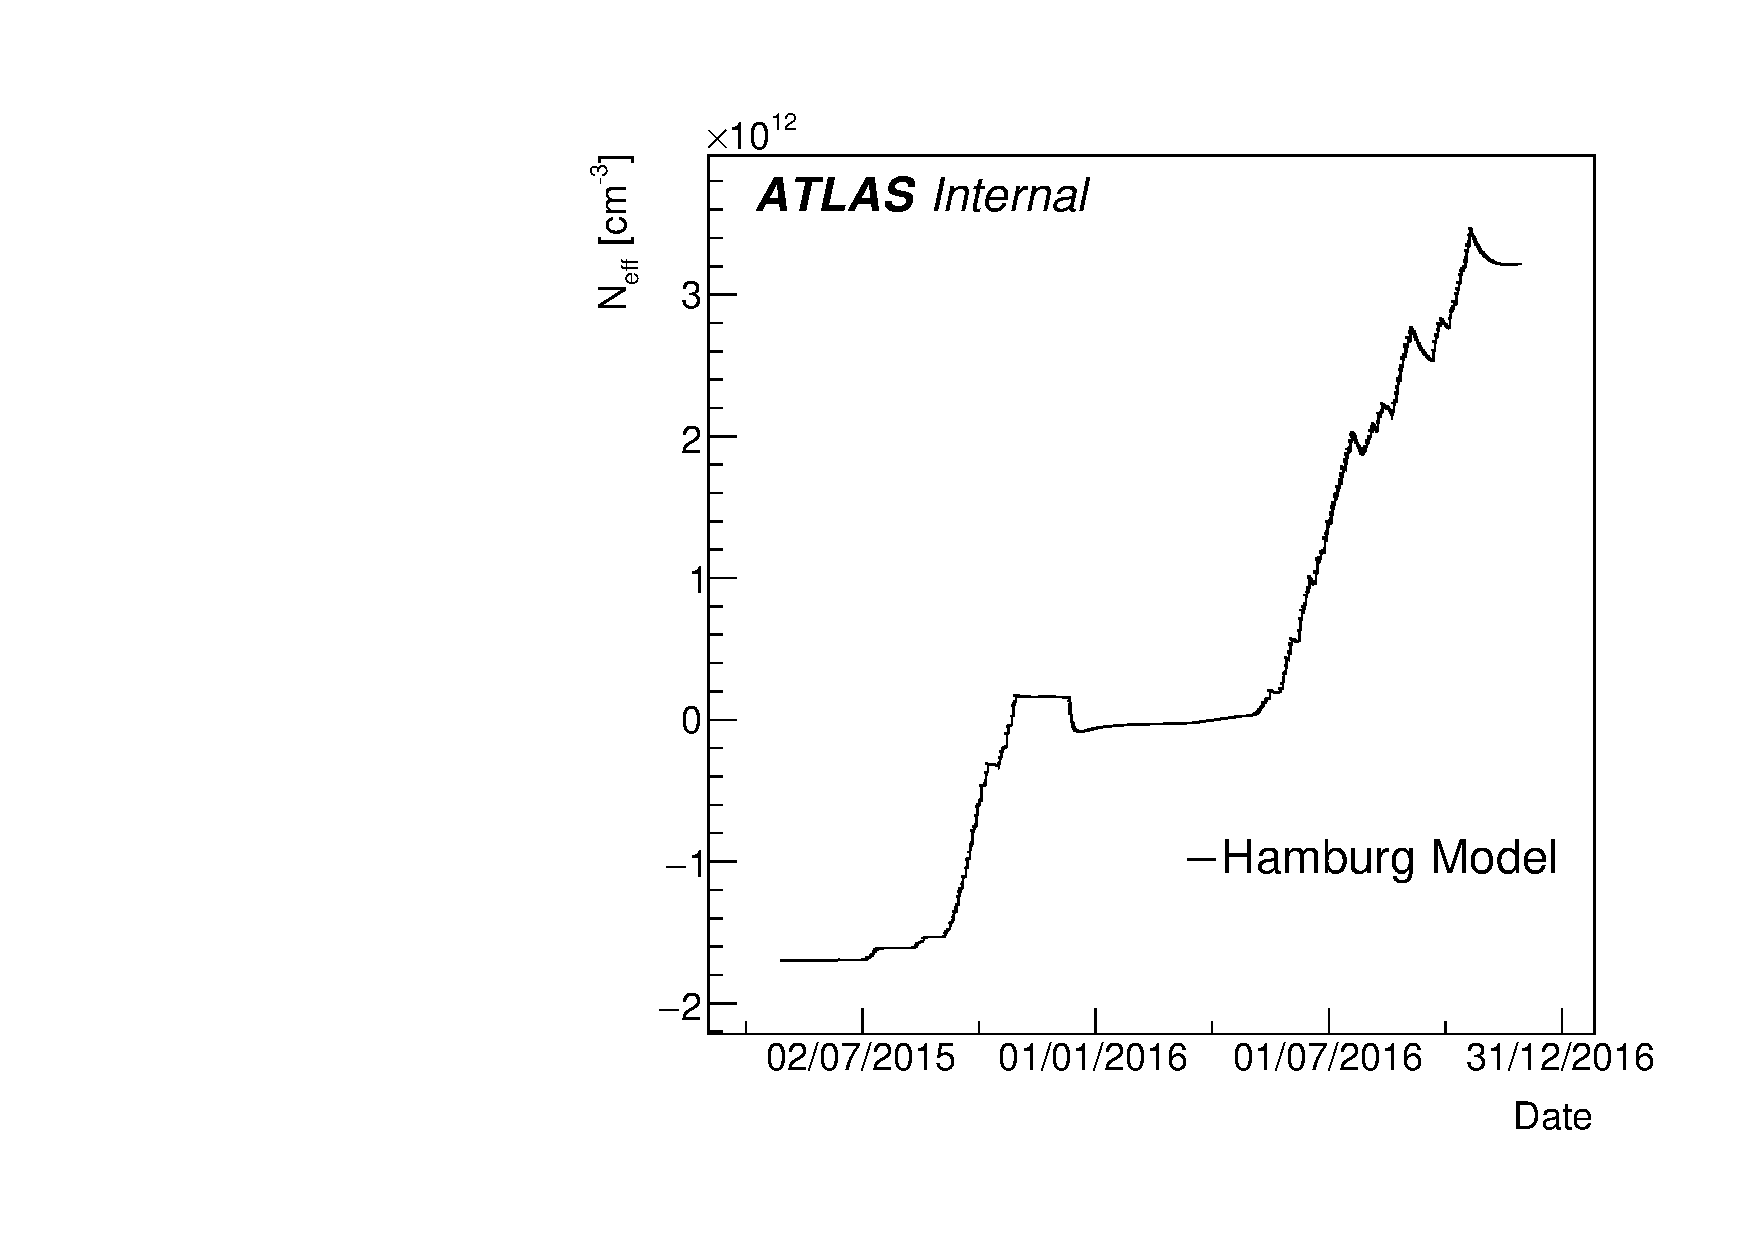
\includegraphics[width=0.55\textwidth]{neff_added}
\caption{The predicted effective doping concentration as a function of time for the IBL using the Hamburg model described in Eq.~\ref{eq:hamburg12}-~\ref{eq:hamburg42}. Donors lead to a negative effective doping concentration while acceptors contribute a positive concentration.  }
\label{fig:electricfield:neff}
\end{figure}

\subsubsection{Depletion Voltage}
\label{sec:depletionvoltage}

The \textit{depletion region} is the volume over which the lifetime of generated carriers is long enough to be collected.  In order to maintain a high charge collection efficiency, it is critical that the depletion region extends to the whole sensor bulk.  The size of this region depends on the bias voltage and the doping concentration, which changes with fluence.   For unirradiated ATLAS planar sensors the depletion region grows from the backside up until type inversion, after which the region grows from the pixel implant.  For highly irradiated sensors, the notion of \textit{fully depleted} is not well-defined since there can be regions inside the sensor bulk that have very low field, even if the top and bottom of the (planar) sensor have a strong electric field.  This is described in more detail in Section~\ref{sec:Efieldprofile}.

 Despite the caveats about depletion at high fluence, at moderate fluences the notion of the depletion region is important for calibrating the Hamburg model that was introduced in Section~\ref{sec:annealing}.  The full depletion voltage in the Hamburg model is defined as the bias voltage fulfilling the following equation:

\begin{align}
\label{eq:hamburg13}
U_\text{full depl.} = |N_\text{eff}| \cdot \frac{ed^2}{2\epsilon\epsilon_0}
\end{align}

where $d$ is the sensor depth. Fig.~\ref{fig:electricfield:depletionvoltage} shows the simulated depletion voltage as a function of time for the IBL
 (left) and b-layer (right). For calibration of the model, measurements with the ATLAS Pixel Detector were obtained by performing bias voltage scans of the mean ToT of hit-clusters on reconstructed particle trajectories. The depletion voltage is extracted by fitting two linear functions to the rising and the plateau region of the measured data. The intersection of the two lines is defined to be the depletion voltage (blue bars in Fig.~\ref{fig:electricfield:depletionvoltage}). Another method which was also used to obtain the full depletion voltage is a scan of the cross-talk between adjacent pixels (green and red bars in Fig.\ref{fig:electricfield:depletionvoltage}, the different colors indicate different information sources). Since the pixels are isolated only after full depletion this is a powerful measurement tool. Unfortunately, this method is only applicable before space-charge sign inversion since otherwise the pixels are isolated already at low bias voltages much before full depletion.

\begin{figure}[!htpb]
\centering
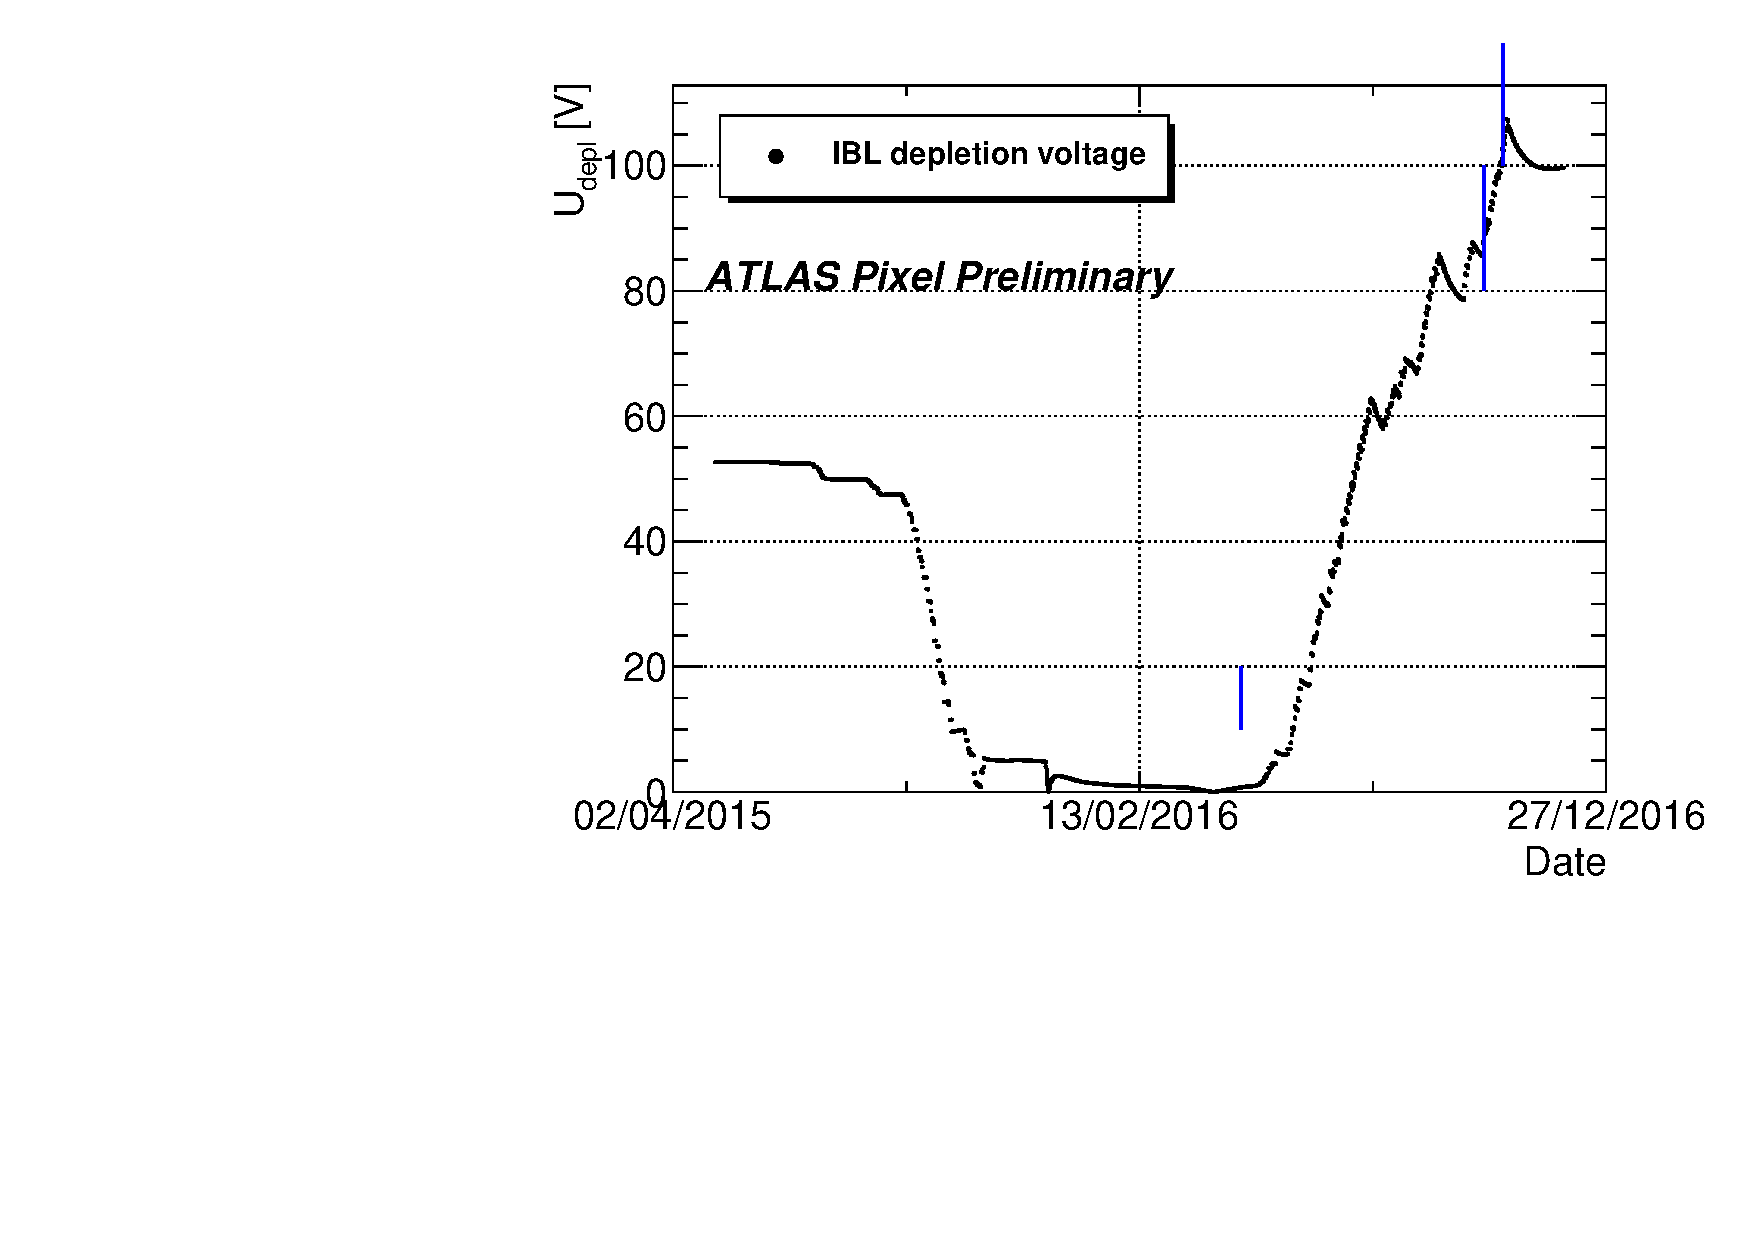
\includegraphics[width=0.45\textwidth]{IBL_2016_new.pdf}
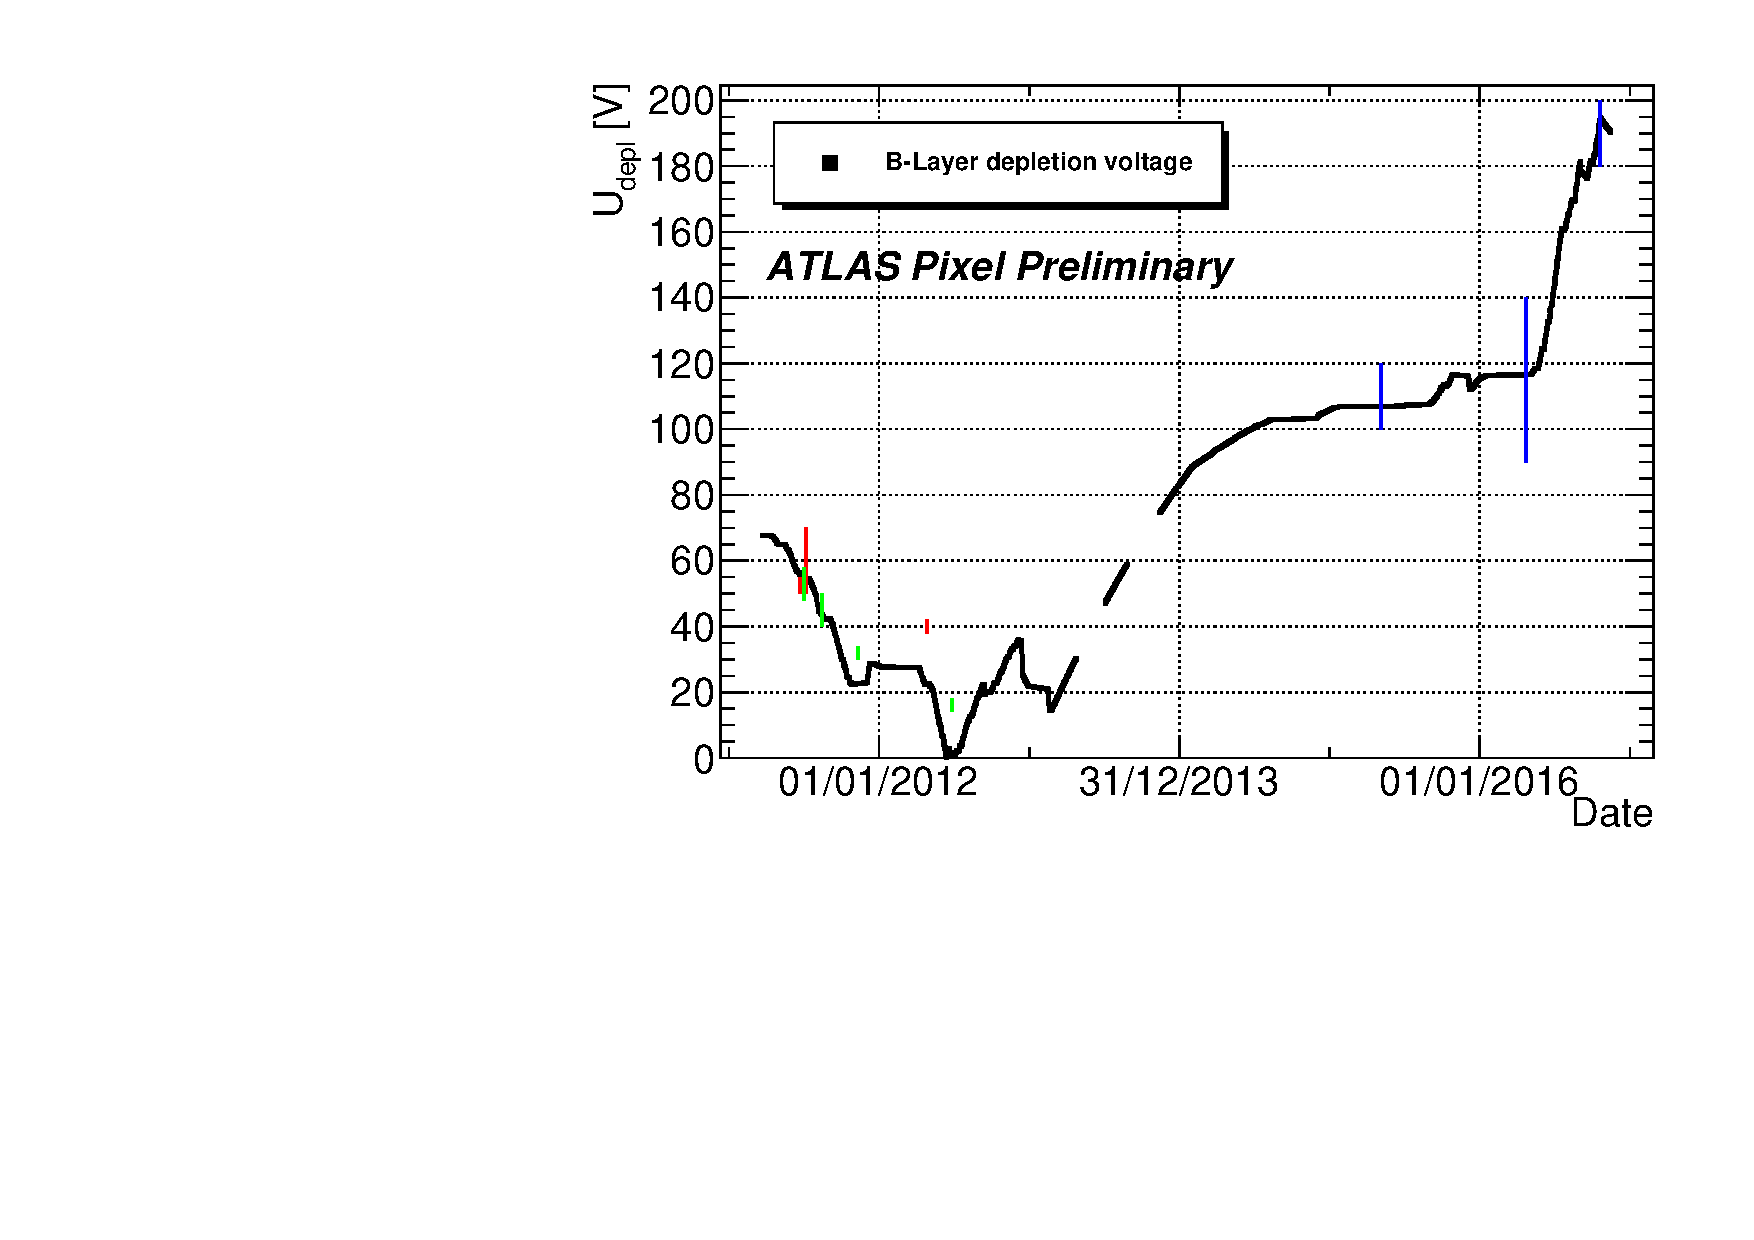
\includegraphics[width=0.45\textwidth]{BLayer_2016_new.pdf}
\caption{Simulated depletion voltage of IBL (left) and b-layer (right) according to the Hamburg model as a function of time from the date of their installation until end of 2016. The shown simulation uses the adapted introduction rates. Blue bars indicate measurements of the depletion voltage using the bias voltage scan method while red and green bars display earlier measurements using cross-talk scans.}
\label{fig:electricfield:depletionvoltage}
\end{figure}

Due to the huge parameter space given by the introduction rates, the time necessary for the simulation, and a focus on physically rather than mathematically correct parameter combinations, the adjustment of the introduction rates was performed by hand. The derived introduction rates are summarized in Table~\ref{tab:depletionvoltage:introductionrates}.  The value of $g_\text{A}$ was chosen close to the literature values since the measurements were done at insensitive points in time with respect to beneficial annealing. The value of $g_\text{Y}$ was estimated from the reverse annealing during the long shutdown 1 (LS1) which was an extended period when the detector was maintained at room temperature. Since the IBL was installed after LS1 and has not undergone significant reverse annealing, the $g_\text{Y}$ value of the b-layer is used also for the IBL. % The simulated depletion voltage was extracted from Fig.~\ref{fig:electricfield:depletionvoltage} at the benchmark fluences which were already crossed and are shown in Table~\ref{tab:depletionvoltage:deplvoltalahamburg}.}

\begin{table}[!htpb]
\centering
\begin{tabular}{|c|c|c|}
  \hline
   Parameter & IBL [$\times 10^{-2} \text{cm}^{-1}$] & B-Layer [$\times 10^{-2} \text{cm}^{-1}$]	\\
   \hline	
$g_\text{A}$ & 1.35 & 1.35\\
$g_\text{Y}$ & 6.0 & 6.0\\
$g_\text{C}$ & 1.1 & 0.45\\
  \hline  
\end{tabular}
\caption{Introduction rates of the Hamburg model as obtained by fitting the simulated depletion voltage to the available measurements.}
\label{tab:depletionvoltage:introductionrates}
\end{table}

For the 3D sensors, the depletion voltage is computed with TCAD using a CV analysis.  The depletion voltage is given by the location in the $1/C^2$ versus $V$ curve where there is a kink (see e.g. Ref.~\cite{rossi2006pixel}).  

Table~\ref{eq:depletionvoltage} lists the bias voltages that are used throughout the rest of the note unless otherwise specified.

\begin{table}[!htpb]
\centering
\begin{tabular}{|c|c|c|}
  \hline
   Fluence ($n_\text{eq}/\text{cm}^2)$ & Depletion Voltage (Planar) (V)& Depletion Voltage (3D)	 (V)	\\
   \hline	
0 & 53 (50) & (-20)\\
$1\times 10^{14}$ & 51 (20) & (-20)\\
$2\times 10^{14}$& 83 (40) & (-30)\\
$5\times 10^{14}$& (125) & (-40)\\
%$1\times 10^{15}$ & -- & -50\\
%$5\times 10^{15}$& -- & -160\\
%$1\times 10^{16}$& -- & -260\\
  \hline  
\end{tabular}
\caption{The calculated depletion voltages as a function of fluence for ATLAS planar and 3D sensors.  For the planar sensors, the depletion voltage is computed using the Hamburg model after determining the introduction rates from Eq.~\ref{eq:hamburg0} by fitting the data.  A fluence of $1\times 10^{14}$ ($2\times 10^{14}$) was reached around 09.07.2016 (08.09.2016).   Values in parentheses are directly from the TCAD simulation based on a CV analysis (prior to the $N_\text{eff}$ correction in the planar case).}
\label{eq:depletionvoltage}
\end{table}

In TCAD radiation damage models like~\cite{bib:DP,CHIOCHIA2006} annealing effects are not included. 
We have devised an effective modelling of annealing of annealing effects for TCAD radiation 
damage models; it will be presented in Section~\ref{sec:TCADAnneal} 

\subsubsection{Field Profiles}
\label{sec:Efieldprofile}

For planar sensors, the field is largely independent of $x$ and $y$, perpendicular to the sensor depth. Figure~\ref{fig:electricfield:profilesRun23} shows the $z$-dependence of the electric field, averaged over $x$ and $y$, for an ATLAS planar sensor for various fluences and a fixed bias voltage of 80 V.  Before irradiation the field is approximately linear, reaching a maximum of about $2V/W\sim 8\times 10^{-4}$ MV/mm, where $V$ is the bias voltage and $W$ is the depletion depth.  After type inversion, the field maximum is on the opposite side of the sensor.  With increasing fluence, there is a minimum in the electric field in the center of the sensor.  For a fluence of $\Phi=5\times 10^{14}$ $n_\text{eq}/\text{cm}^2$ for 80 V (under-depleted - see Section~\ref{sec:depletionvoltage}), this minimum is broad and occupies nearly a third of the sensor.

Analogous distributions for 3D sensors are shown in Fig.~\ref{fig:electricfield:profilesRun23_3D}.  In contrast to planar sensors, the field is nearly independent of $z$ and depends strongly on $x$ and $y$.  Therefore, the electric field magnitude is shown as a two-dimensional map for both an unirradiated sensor and a highly irradiated sensor.  The $n^+$ and $p^+$ implants are regions of no field due to their large doping, as are locations in the sensor that are geometrically between two implants of opposite polarity.  To illustrate the entire pixel, the one-eighth map that is simulated is tessellated (Section~\ref{sec:ElectricField:SimulationDetails}).

\begin{figure}[!htpb]
\centering
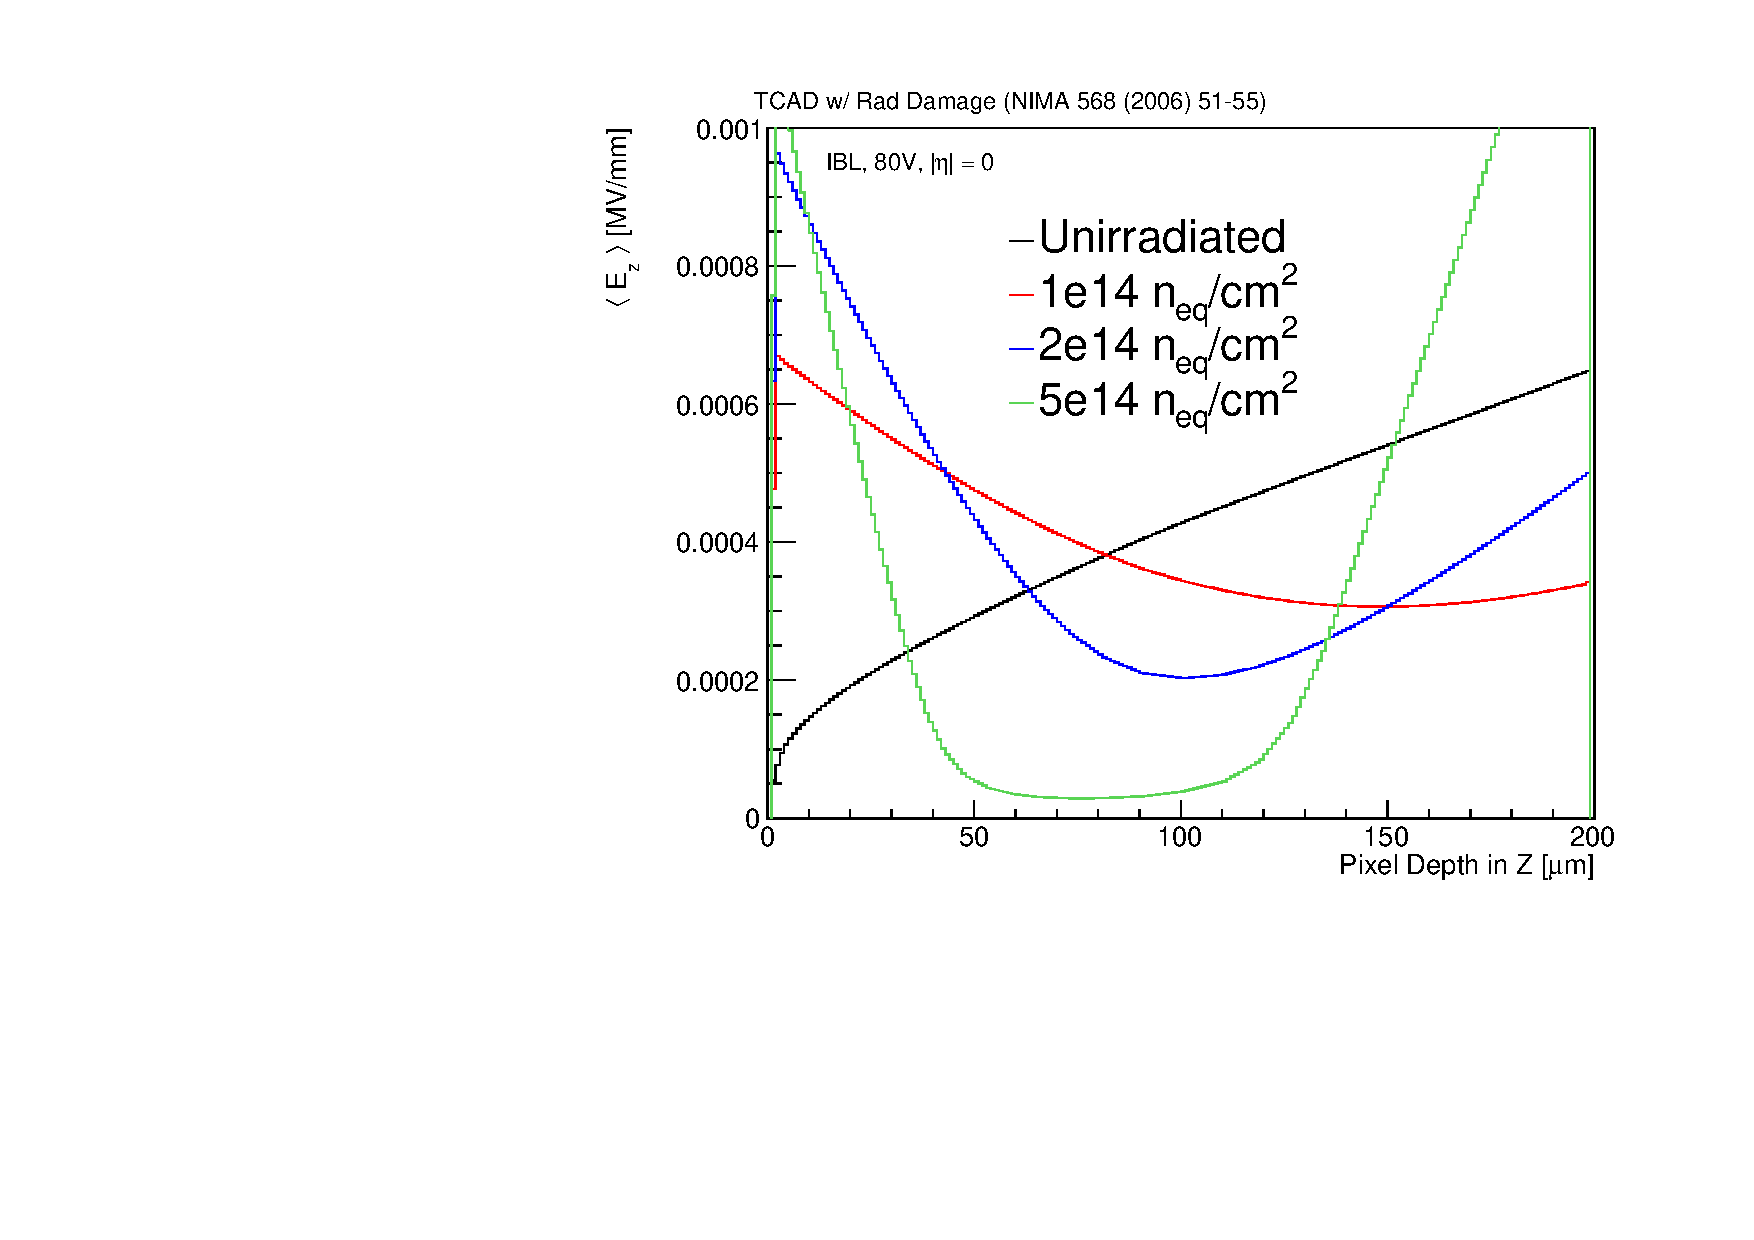
\includegraphics[width=0.6\textwidth]{Ez_0fluence80V.pdf}
\caption{The electric field magnitude in the $z$ direction, averaged over $x$ and $y$ for a the ATLAS IBL sensor biased at 80 V and at various fluences.}
\label{fig:electricfield:profilesRun23}
\end{figure}

\begin{figure}[!htpb]
\centering
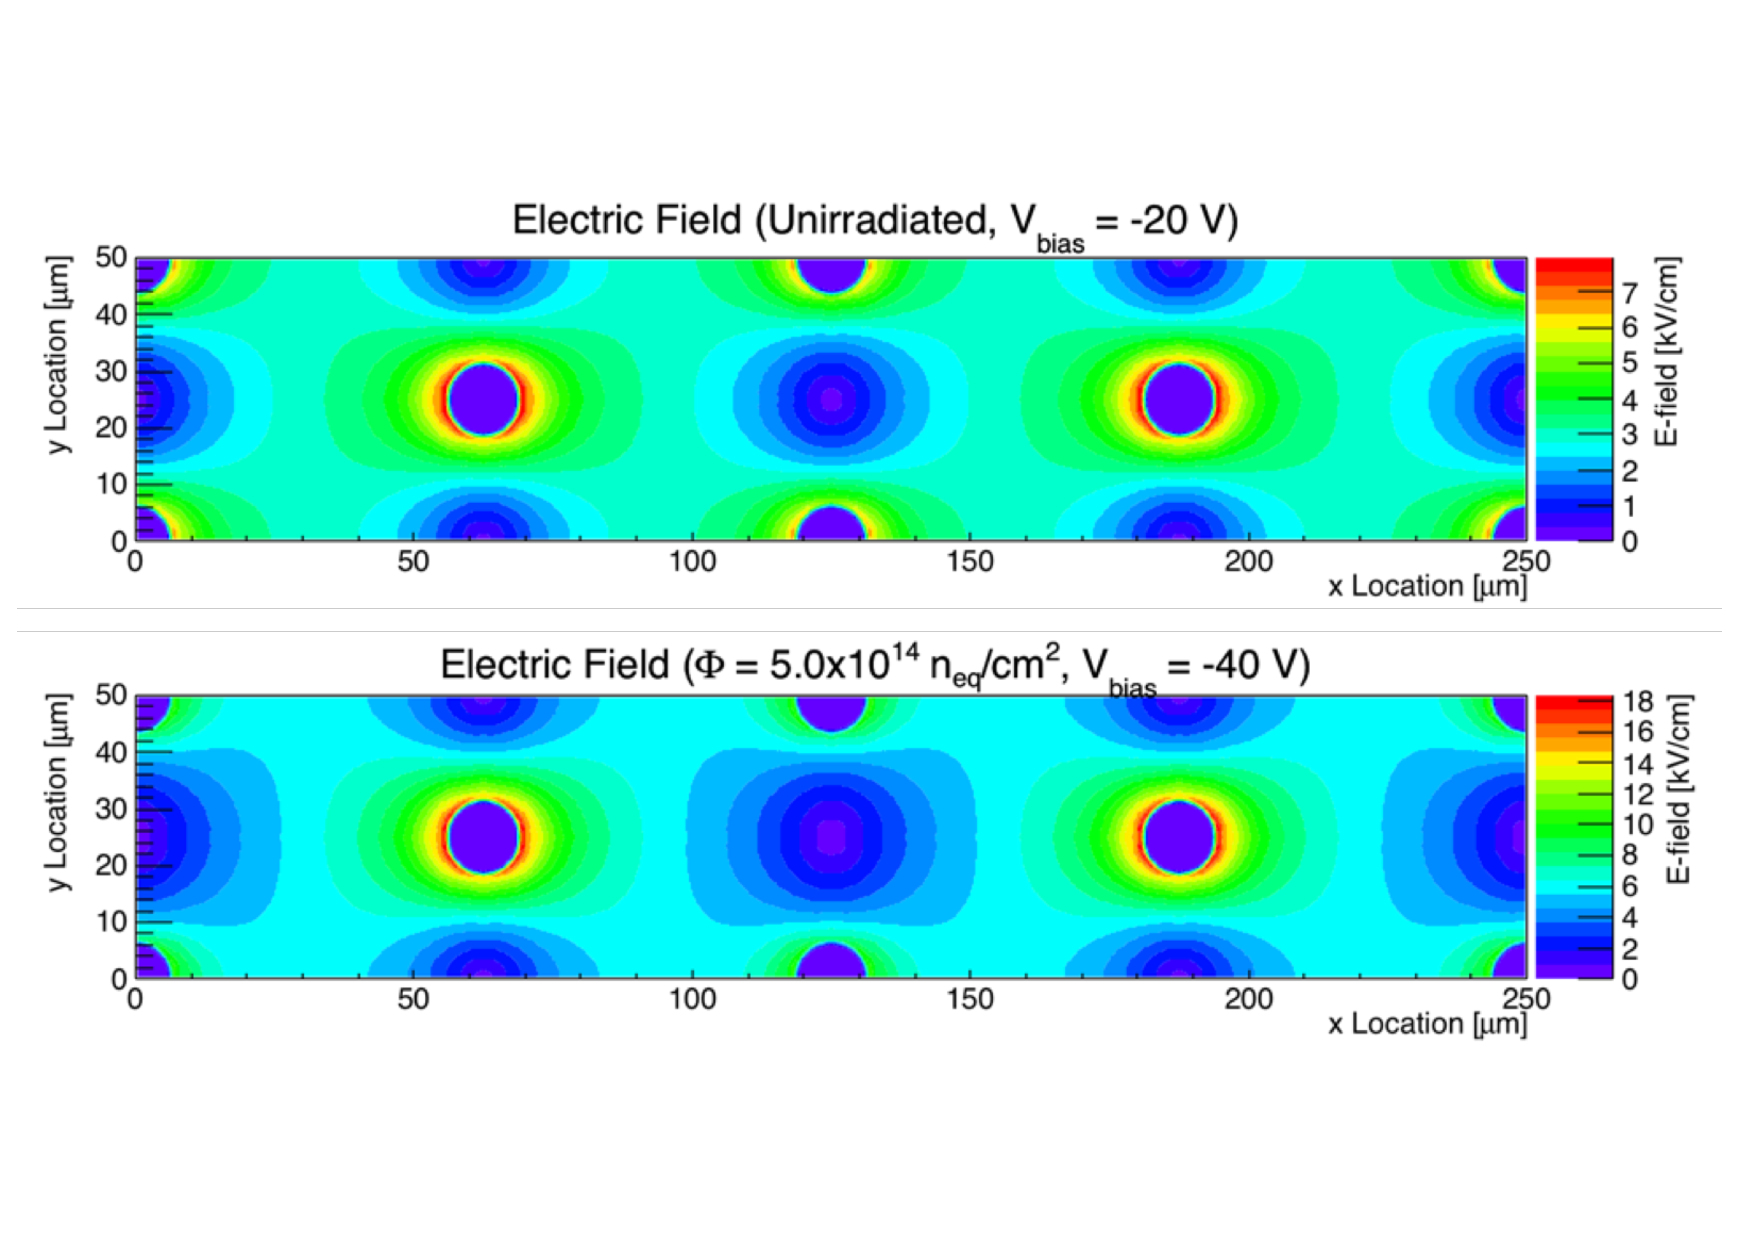
\includegraphics[width=0.95\textwidth]{Figure7.pdf}
\caption{The magnitude of the electric field as a function of local $x$ and $y$ in an ATLAS IBL 3D sensor for an unirradiated sensor (top) and for a fluence of $5\times10^{14}$ $n_\text{eq}/\text{cm}^2$ (bottom). }
\label{fig:electricfield:profilesRun23_3D}
\end{figure}

\subsubsection{Model Comparisons}
\label{sec:Efieldmodelcomparisons}

Extensive model comparisons are beyond the scope of this note, but the data presented in Sec.~\ref{sec:digivalidation} can be used to constrain various simulations as well as tune parameters and derive systematic uncertainties for predictions for higher luminosity data.  In addition to the Chiochia model for the planar sensors, the Petasecca model was also briefly investigated.  While the model itself is supported by testbeam data~\cite{1710302}, it is found to disagree qualitatively on the fluence for type-inversion with the Chiochia model and does not display a two-peaked electric field profile after irradiation.  Therefore, this alternative model was not studied in further detail.

Next, Chiochia model parameters are varied.
The summary of the parameters variations is presented in Table~\ref{tab:parVars}.

\begin{table}[!htpb]
\centering
\begin{tabular}{|l|c|c|c|c|}
  \hline
  State/variation & $\eta$ & $E_t$ & $\sigma_e$ & $\sigma_h$		\\
   \hline	
   acceptor & $\pm 10\%$ & $\sim\pm0.4\%$ & $\pm10\%$ & $\pm10\%$ \\
   donor & $\pm 10\%$ & $\sim\pm0.4\%$ & $\pm10\%$ & $\pm10\%$ \\
  \hline  
\end{tabular}
\caption{Variations of Chiochia model~\cite{Chiochia:2004qh} parameters.}
\label{tab:parVars}
\end{table}

Figures~\ref{fig:acc_electricfieldvariations} and~\ref{fig:don_electricfieldvariations} show the electric field for variations in respectively the acceptor and donor trap parameters for a fluence of $10^{14}$ $n_\text{eq}/\text{cm}^2$ and a bias voltage of~80 V.  The normalization of all the curves is fixed by the bias voltage and therefore all the curves cross at a point. 


\begin{figure}[htpb!]
\centering
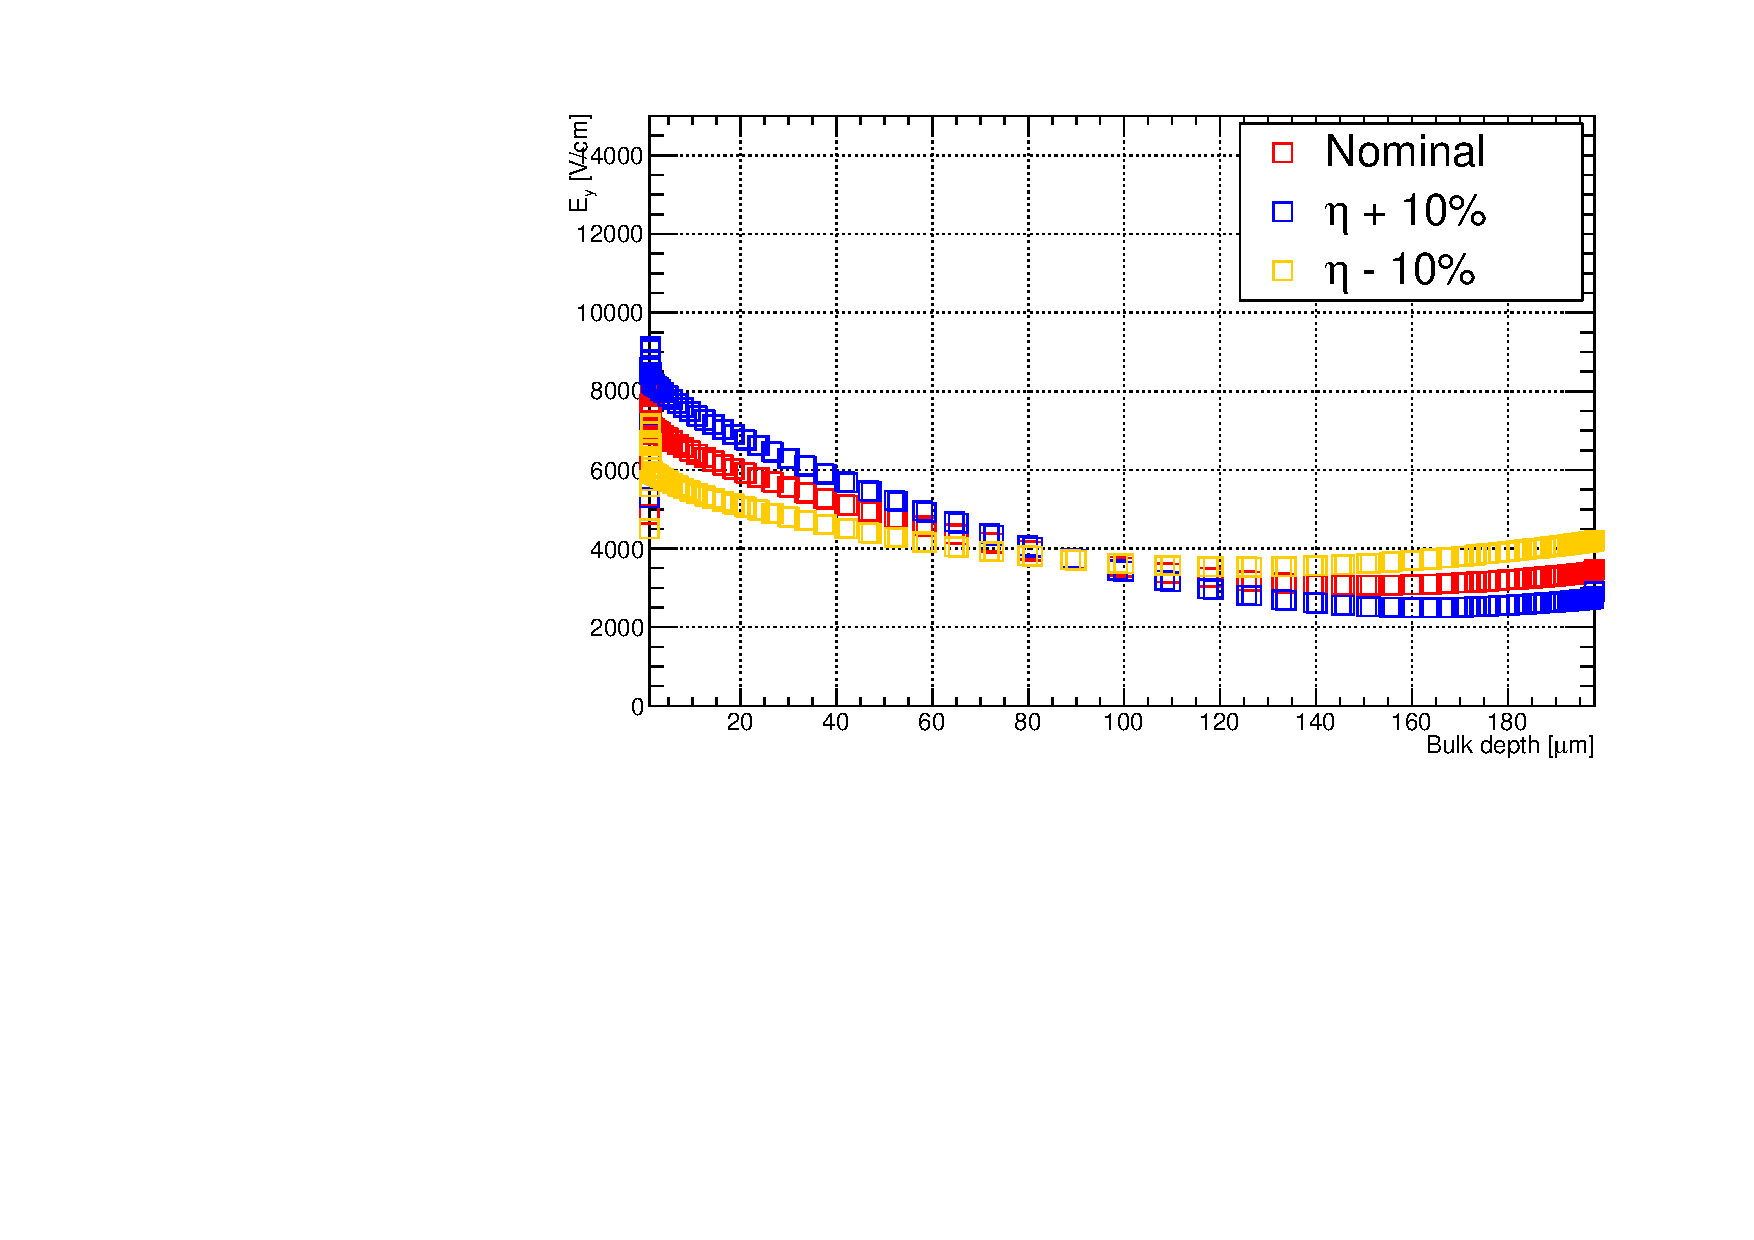
\includegraphics[width=0.49\textwidth]{new_Aetavariation.pdf}
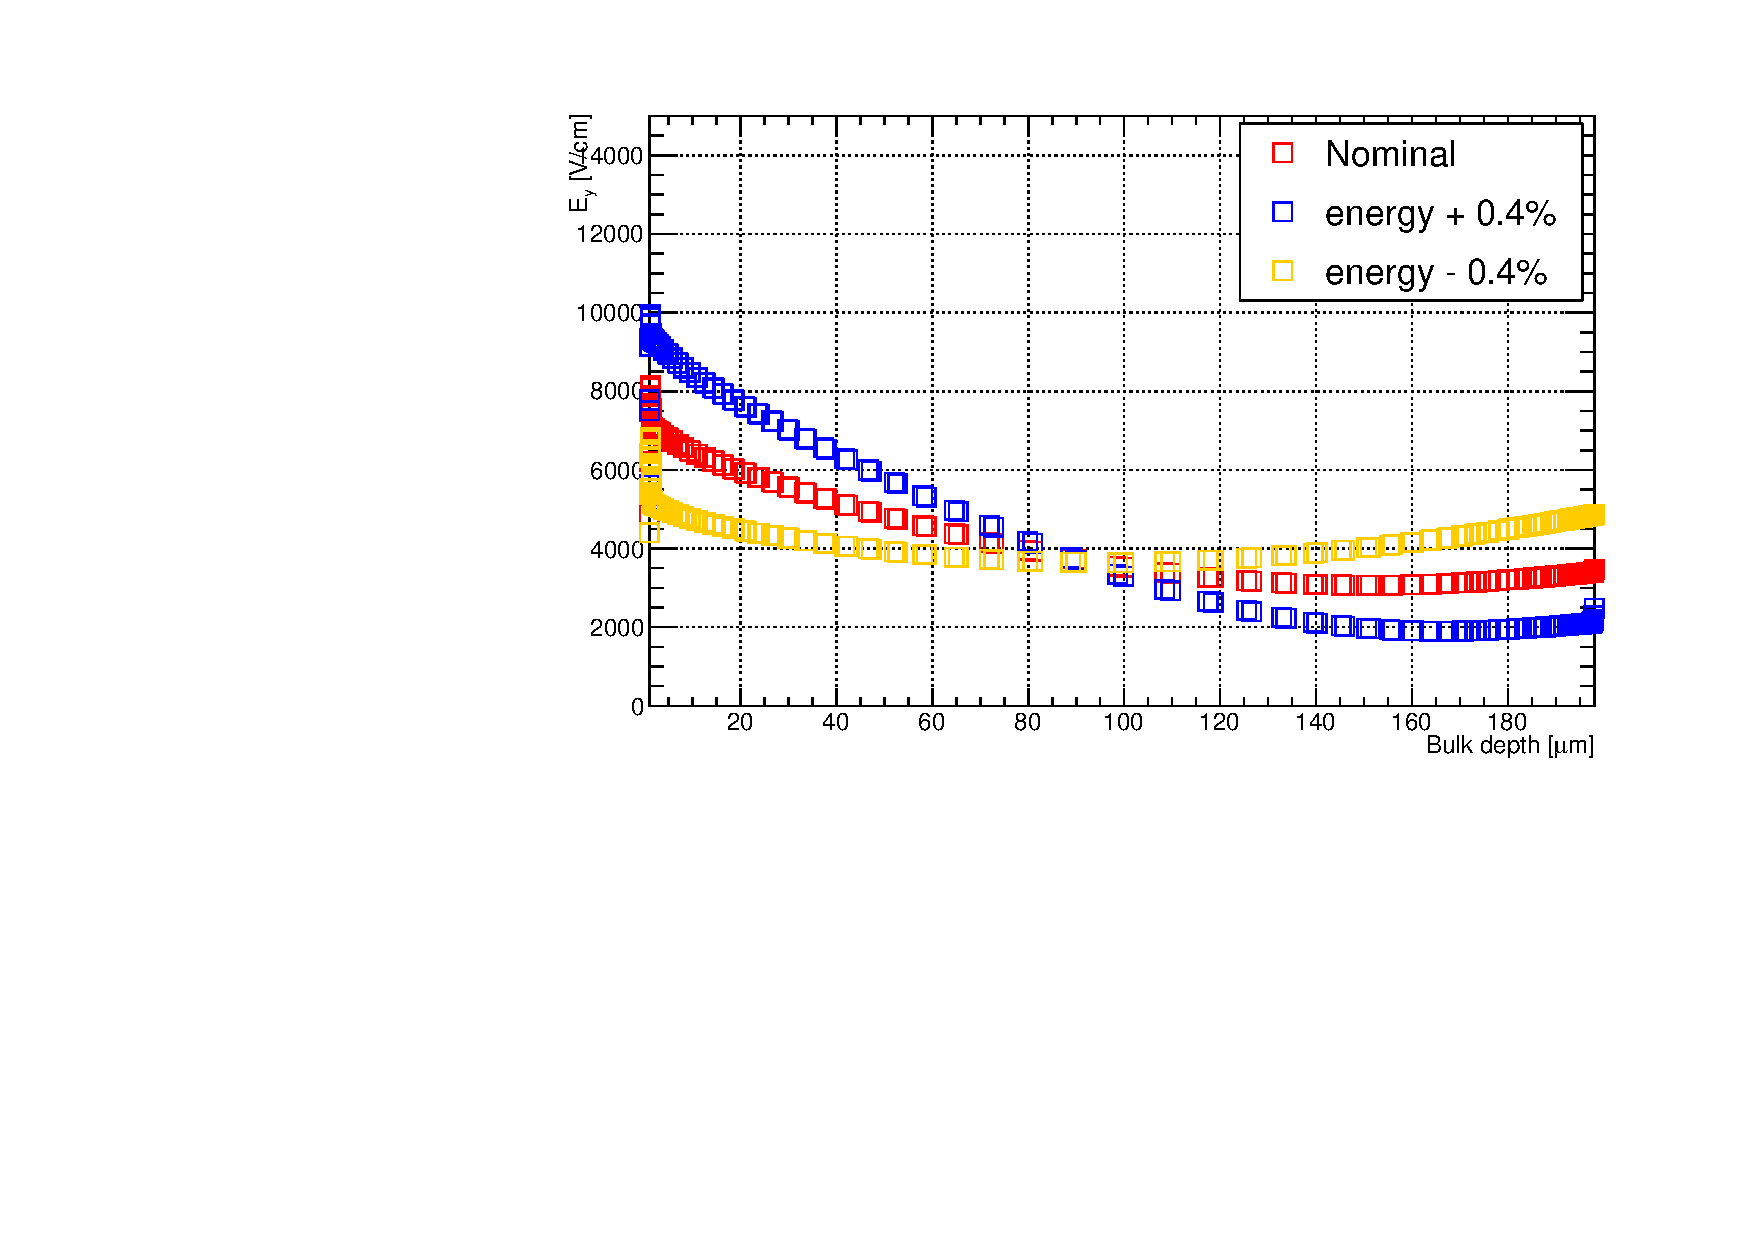
\includegraphics[width=0.49\textwidth]{new_Aenergyvariation.pdf}
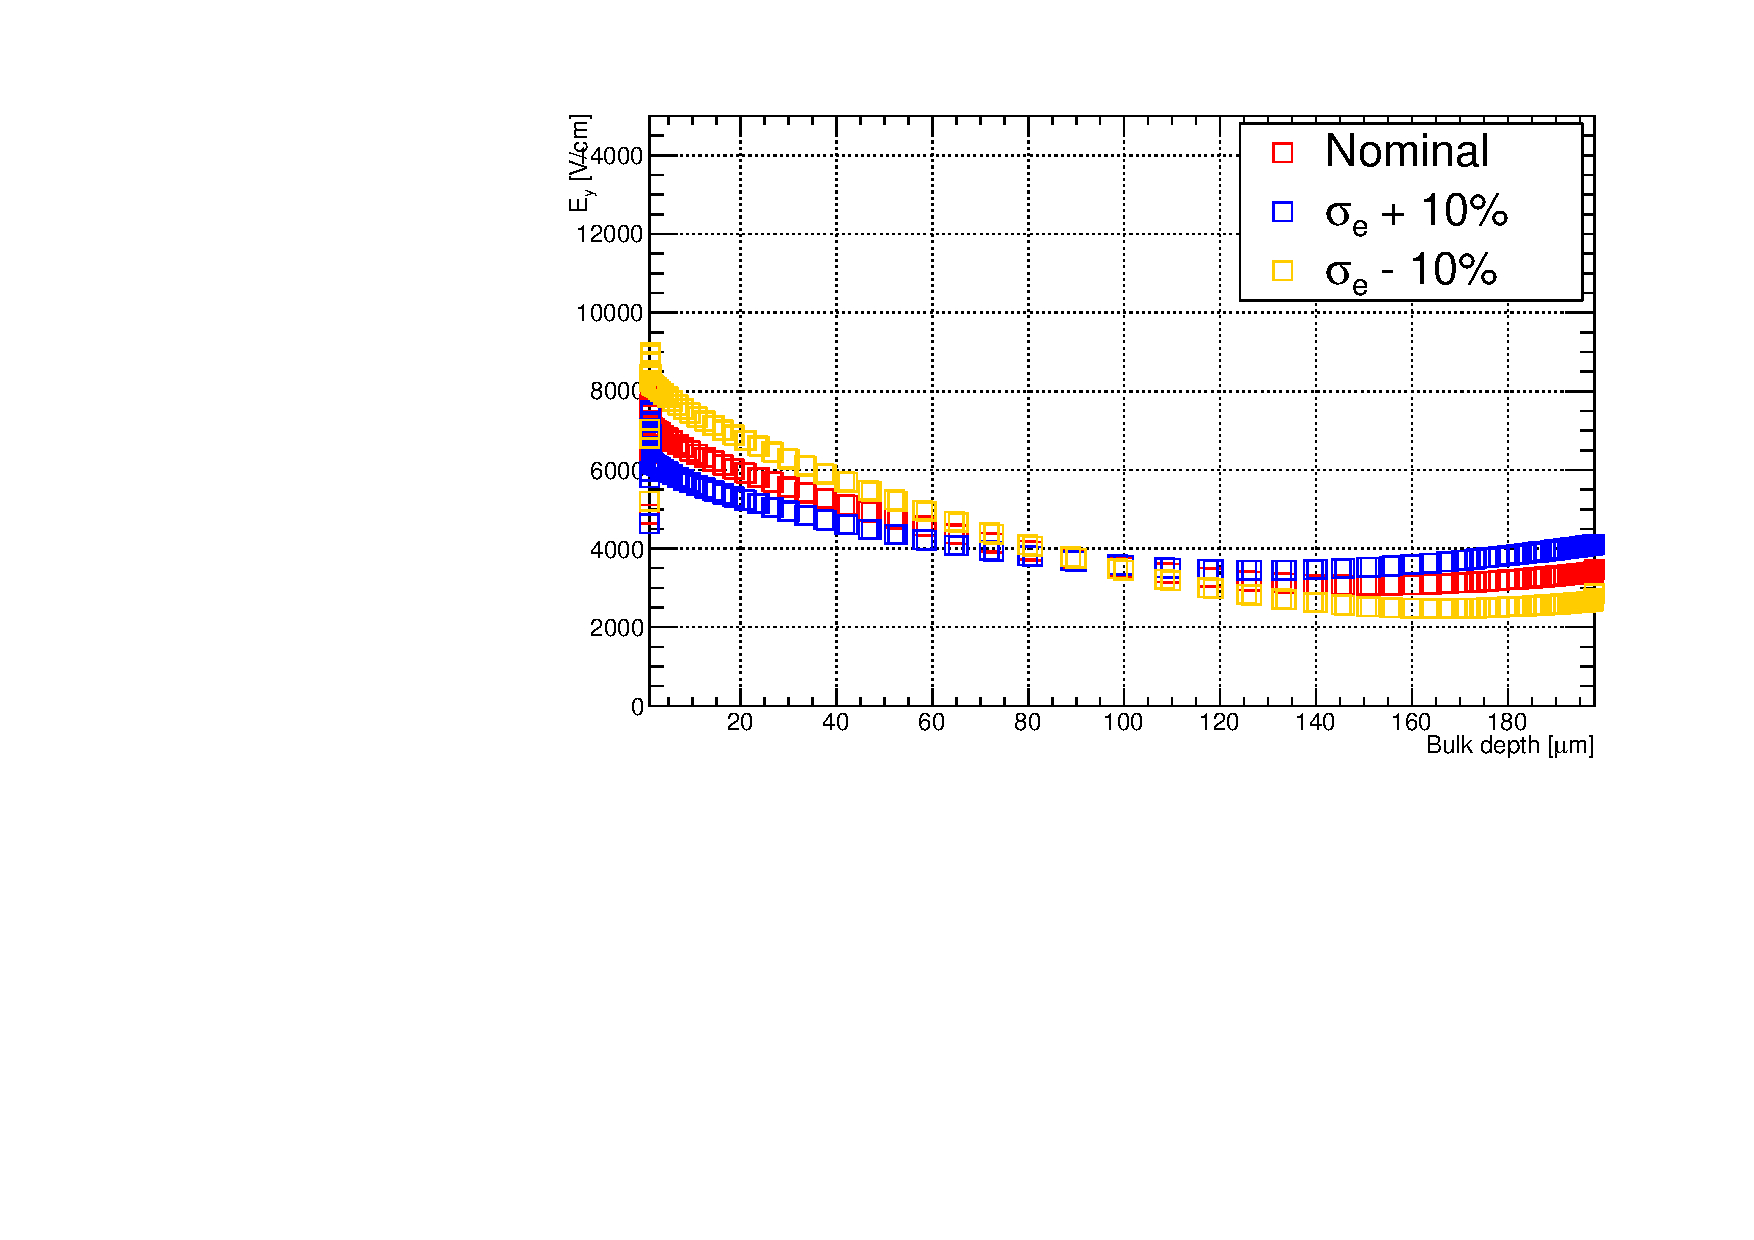
\includegraphics[width=0.49\textwidth]{new_Asigmaevariation.pdf}
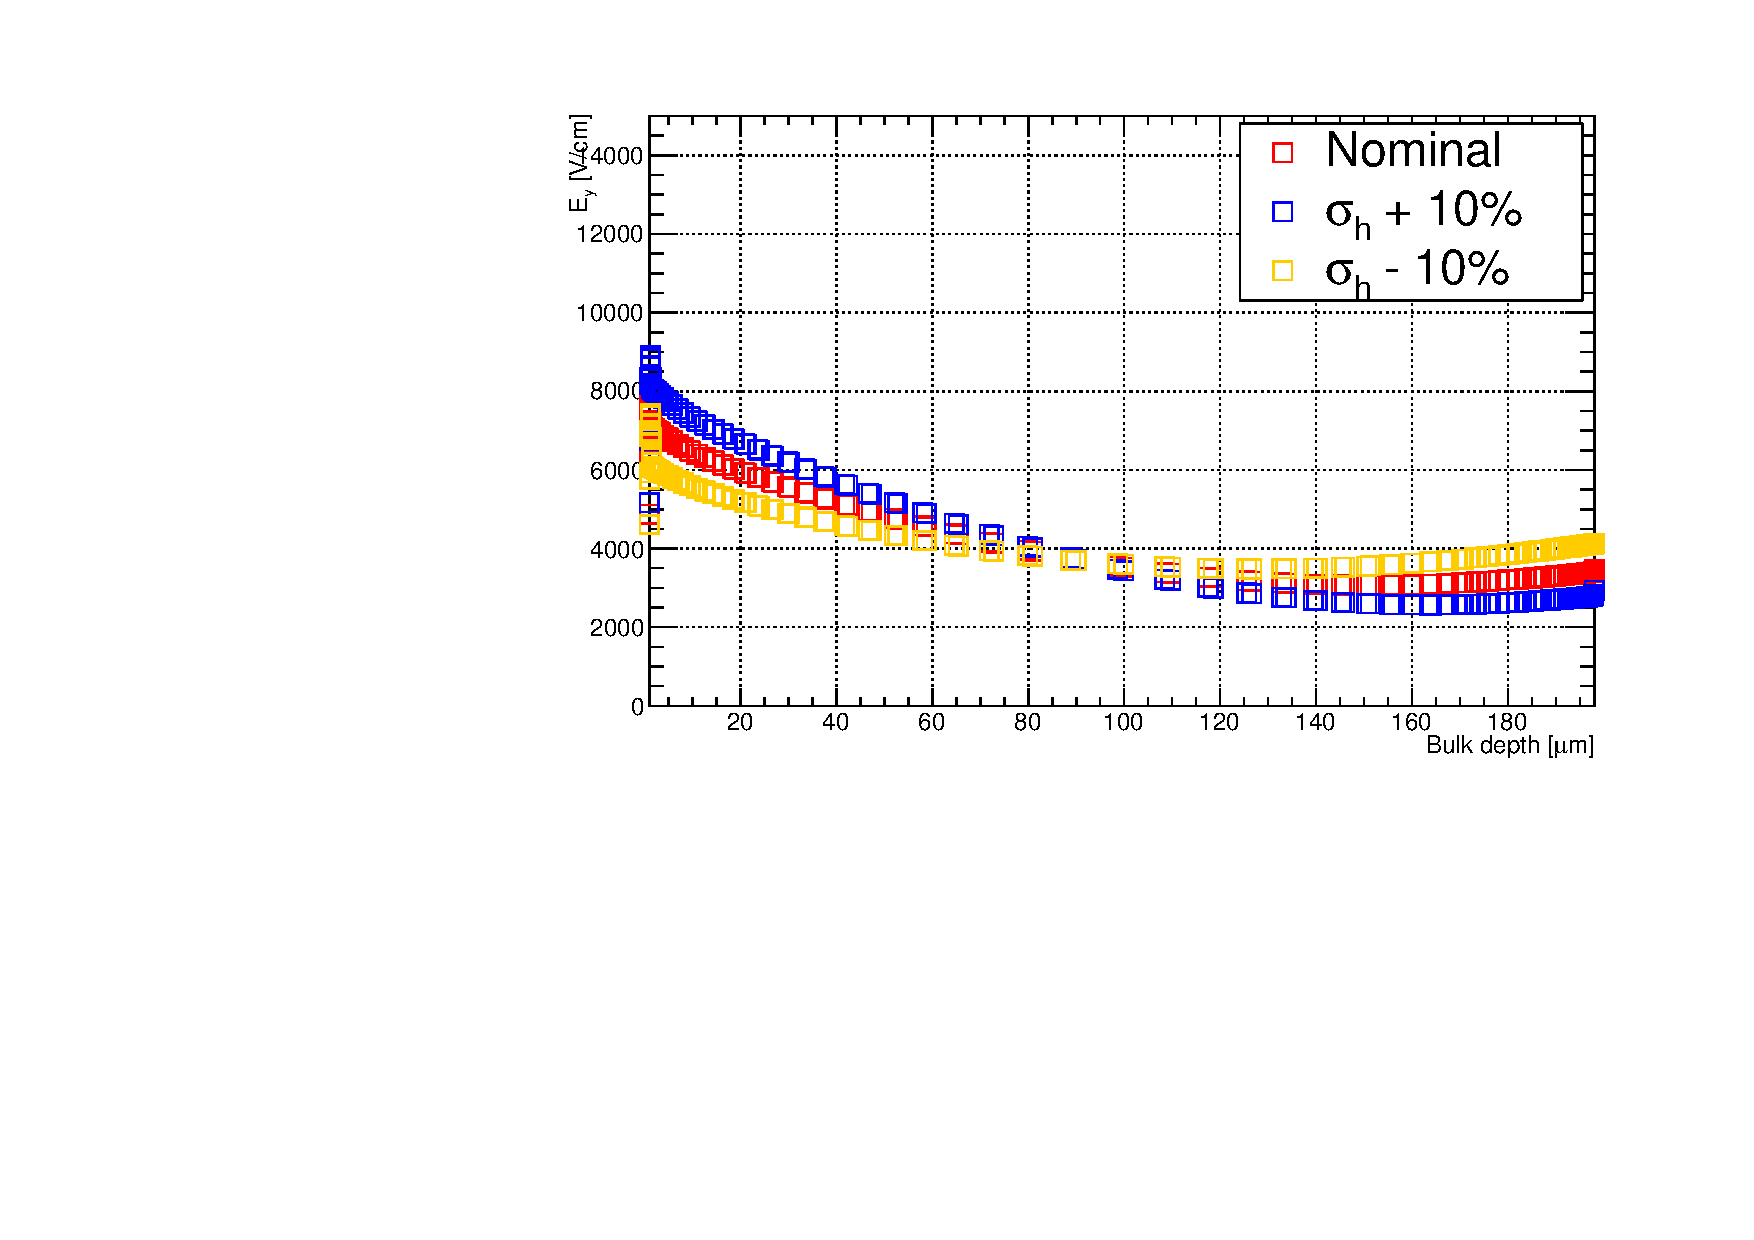
\includegraphics[width=0.49\textwidth]{new_Asigmahvariation.pdf}
\caption{The $z$ dependence of the electric field in an ATLAS planar sensor, averaged over $x$ and $y$, for a simulated
  fluence of $\Phi=1\times10^{14}$~(1~MeV)~n$_\text{eq}/\text{cm}^{2}$, after varying parameters of the acceptor trap in the Chiochia model. (Top) The left plot shows a $\pm 10\%$ variation in the fluence dependence of the acceptor trap concentrations while the right plot shows a variation in the acceptor trap energy level by $0.4\%$. 
  (Bottom) The left plot shows a $\pm 10\%$ variation in the electron capture cross section, the right one a $\pm 10\%$ variation in the hole capture cross section.
The bias voltage was set to $80$ V in all cases.}
\label{fig:acc_electricfieldvariations}
\end{figure}


\begin{figure}[htpb!]
\centering
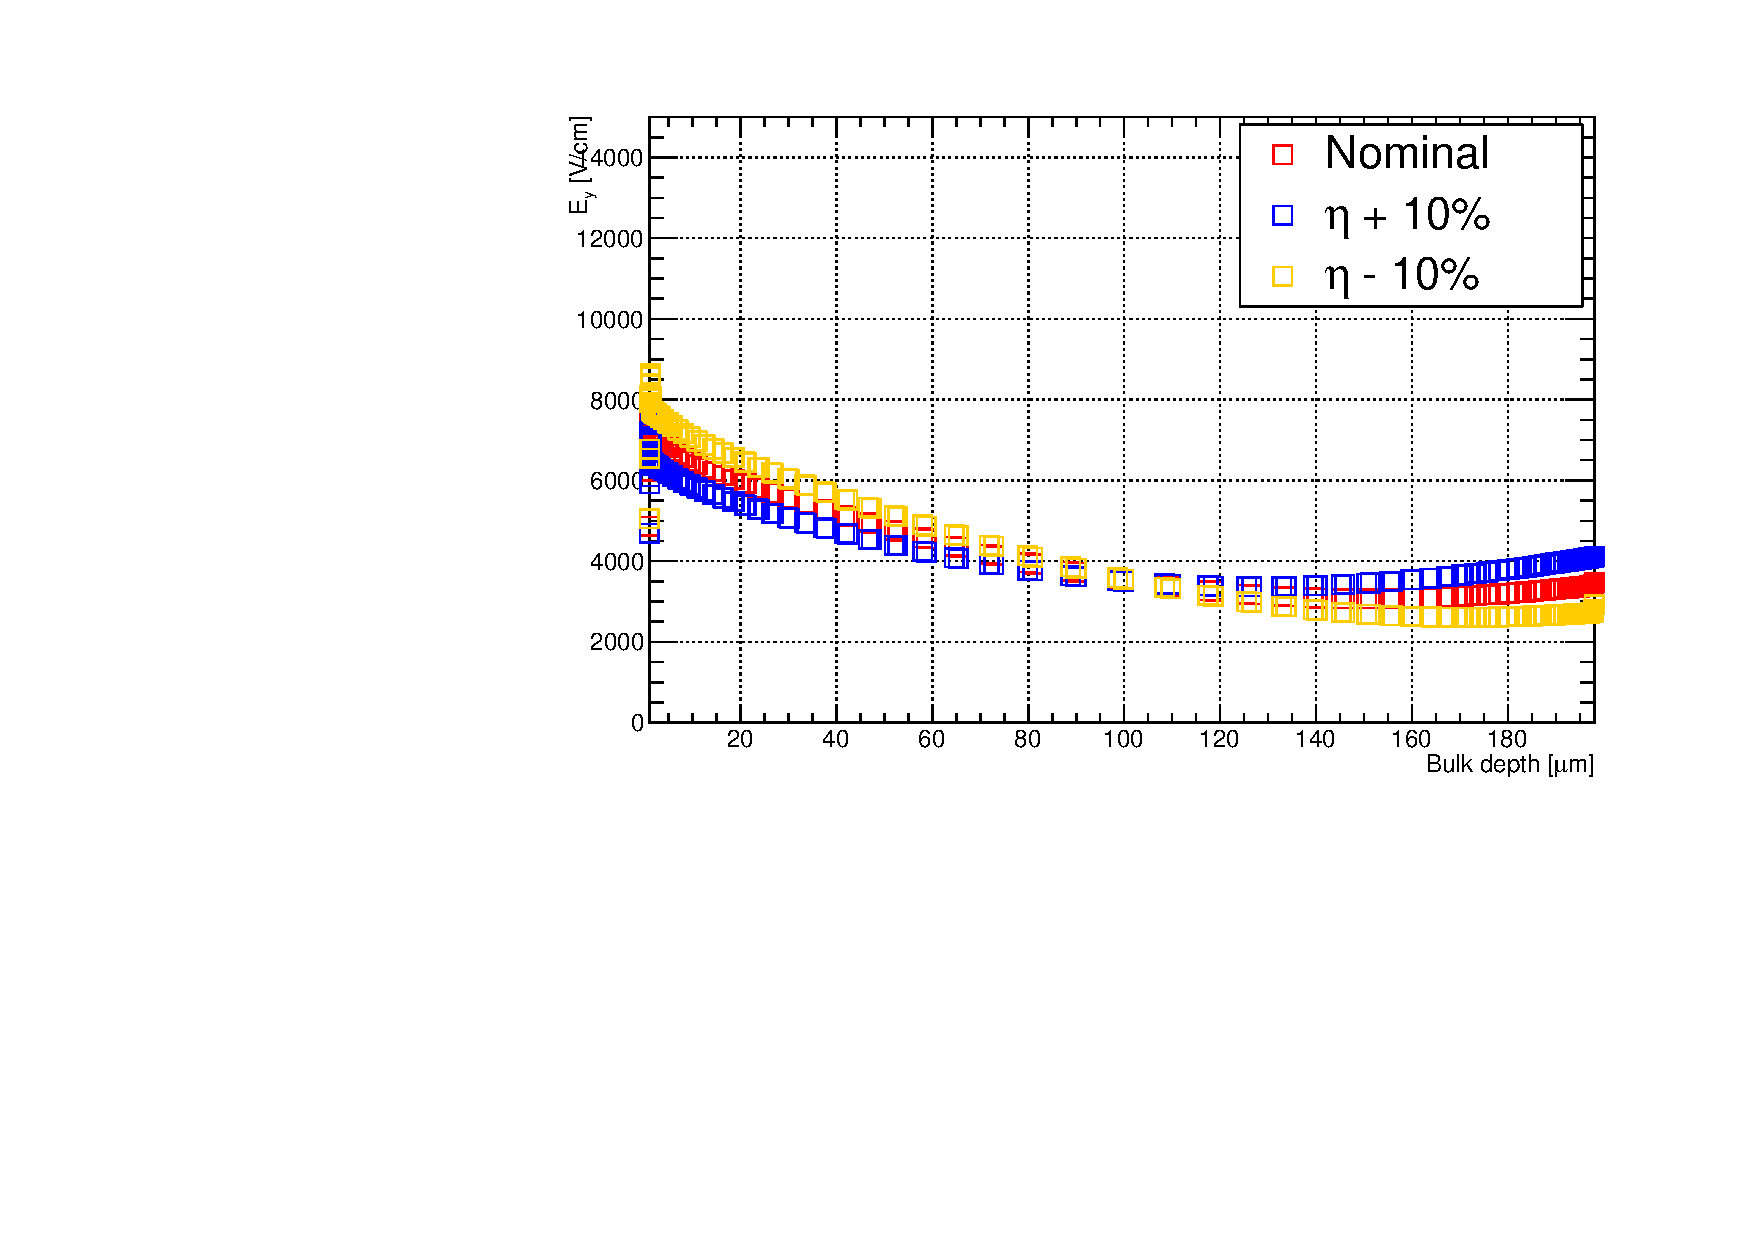
\includegraphics[width=0.49\textwidth]{new_Detavariation.pdf}
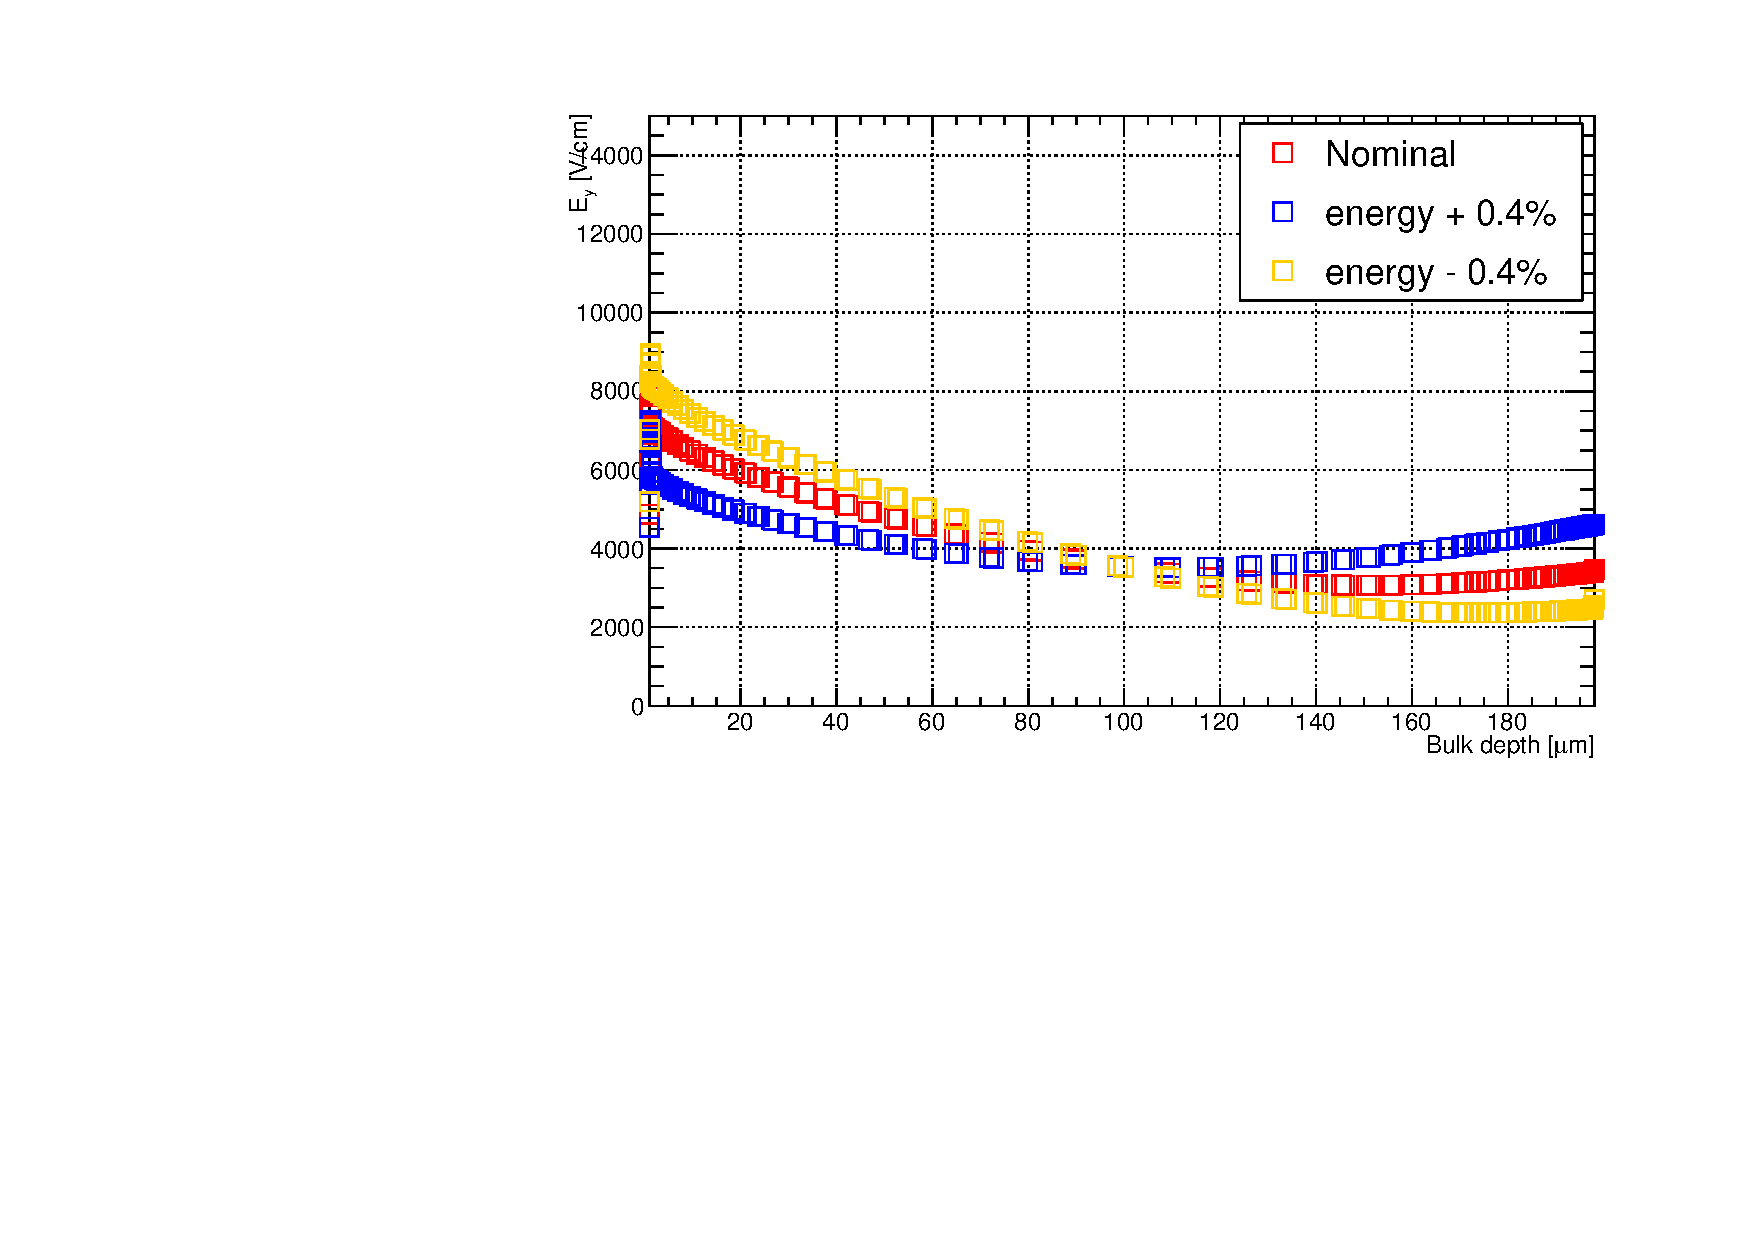
\includegraphics[width=0.49\textwidth]{new_Denergyvariation.pdf}
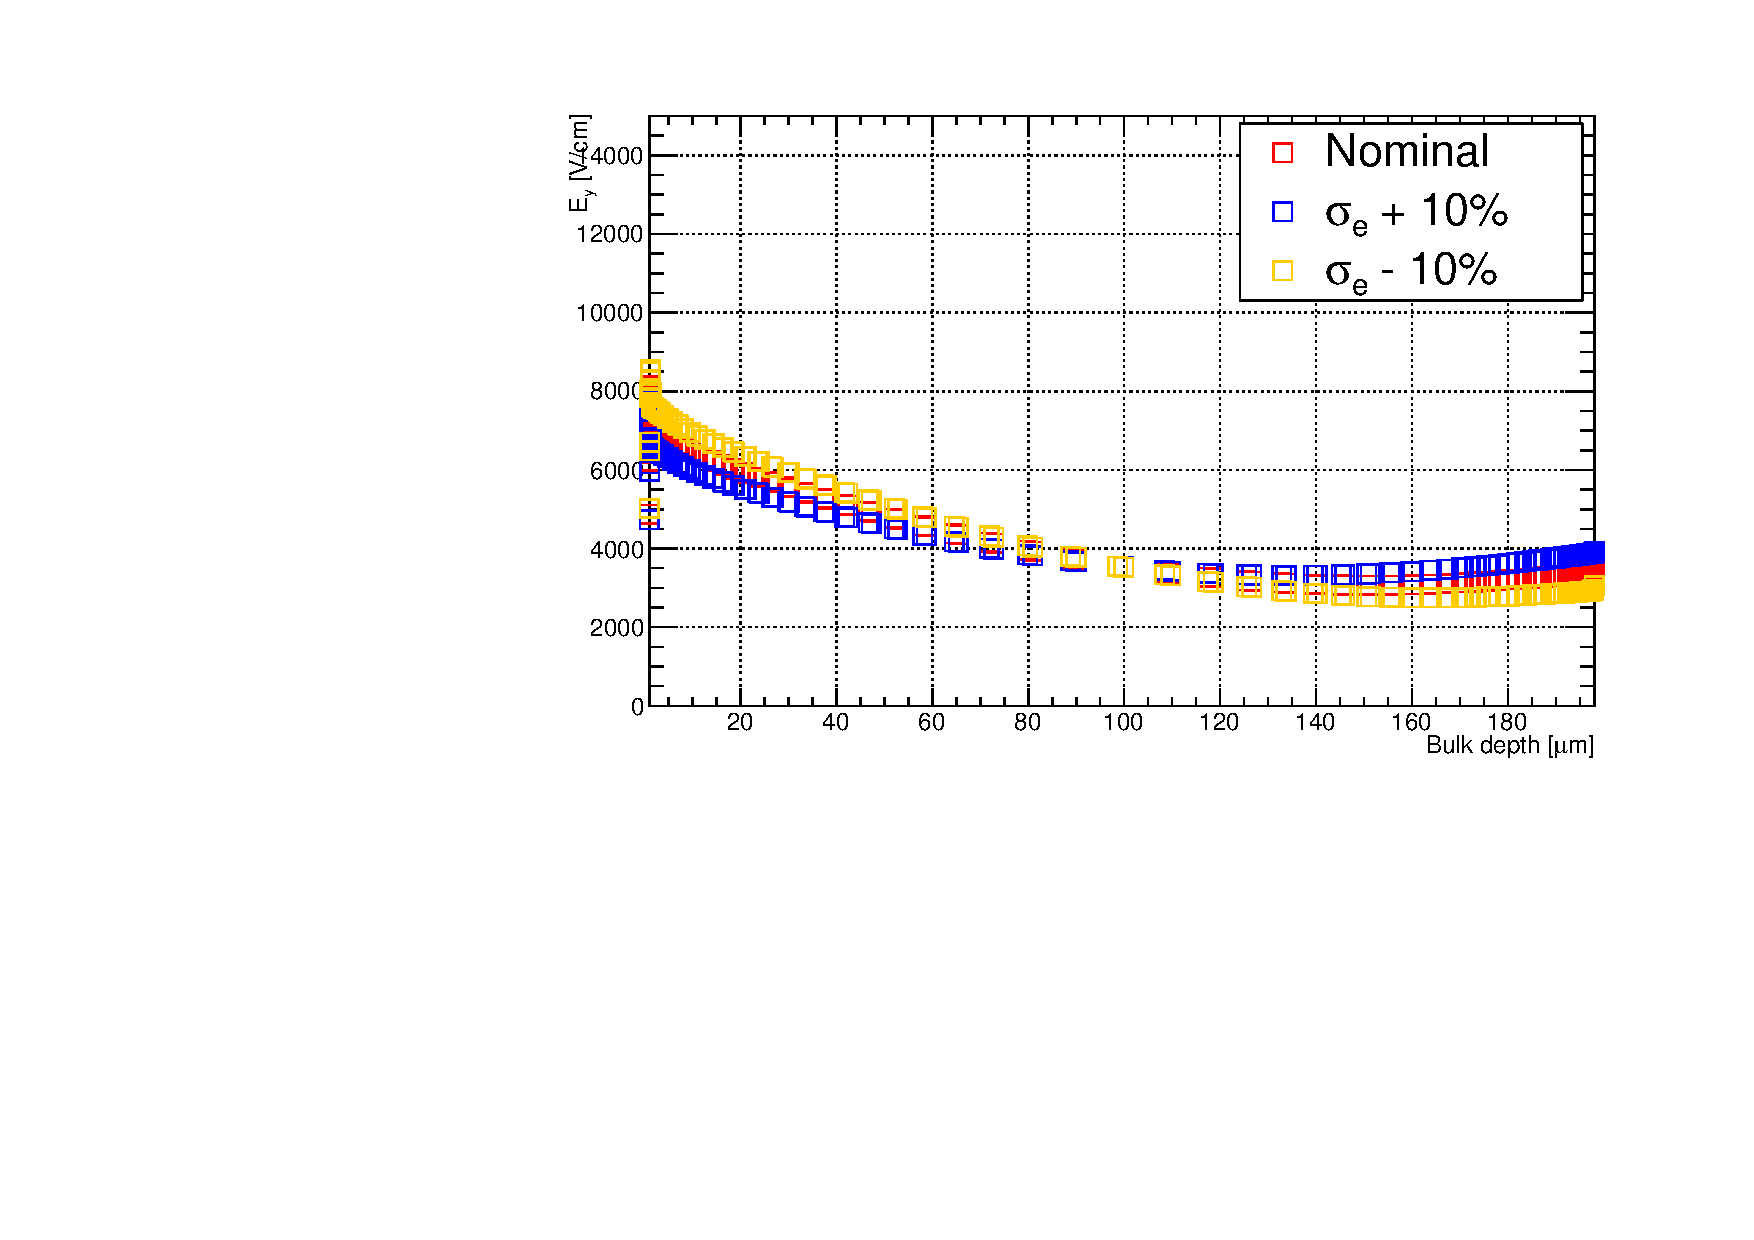
\includegraphics[width=0.49\textwidth]{new_Dsigmaevariation.pdf}
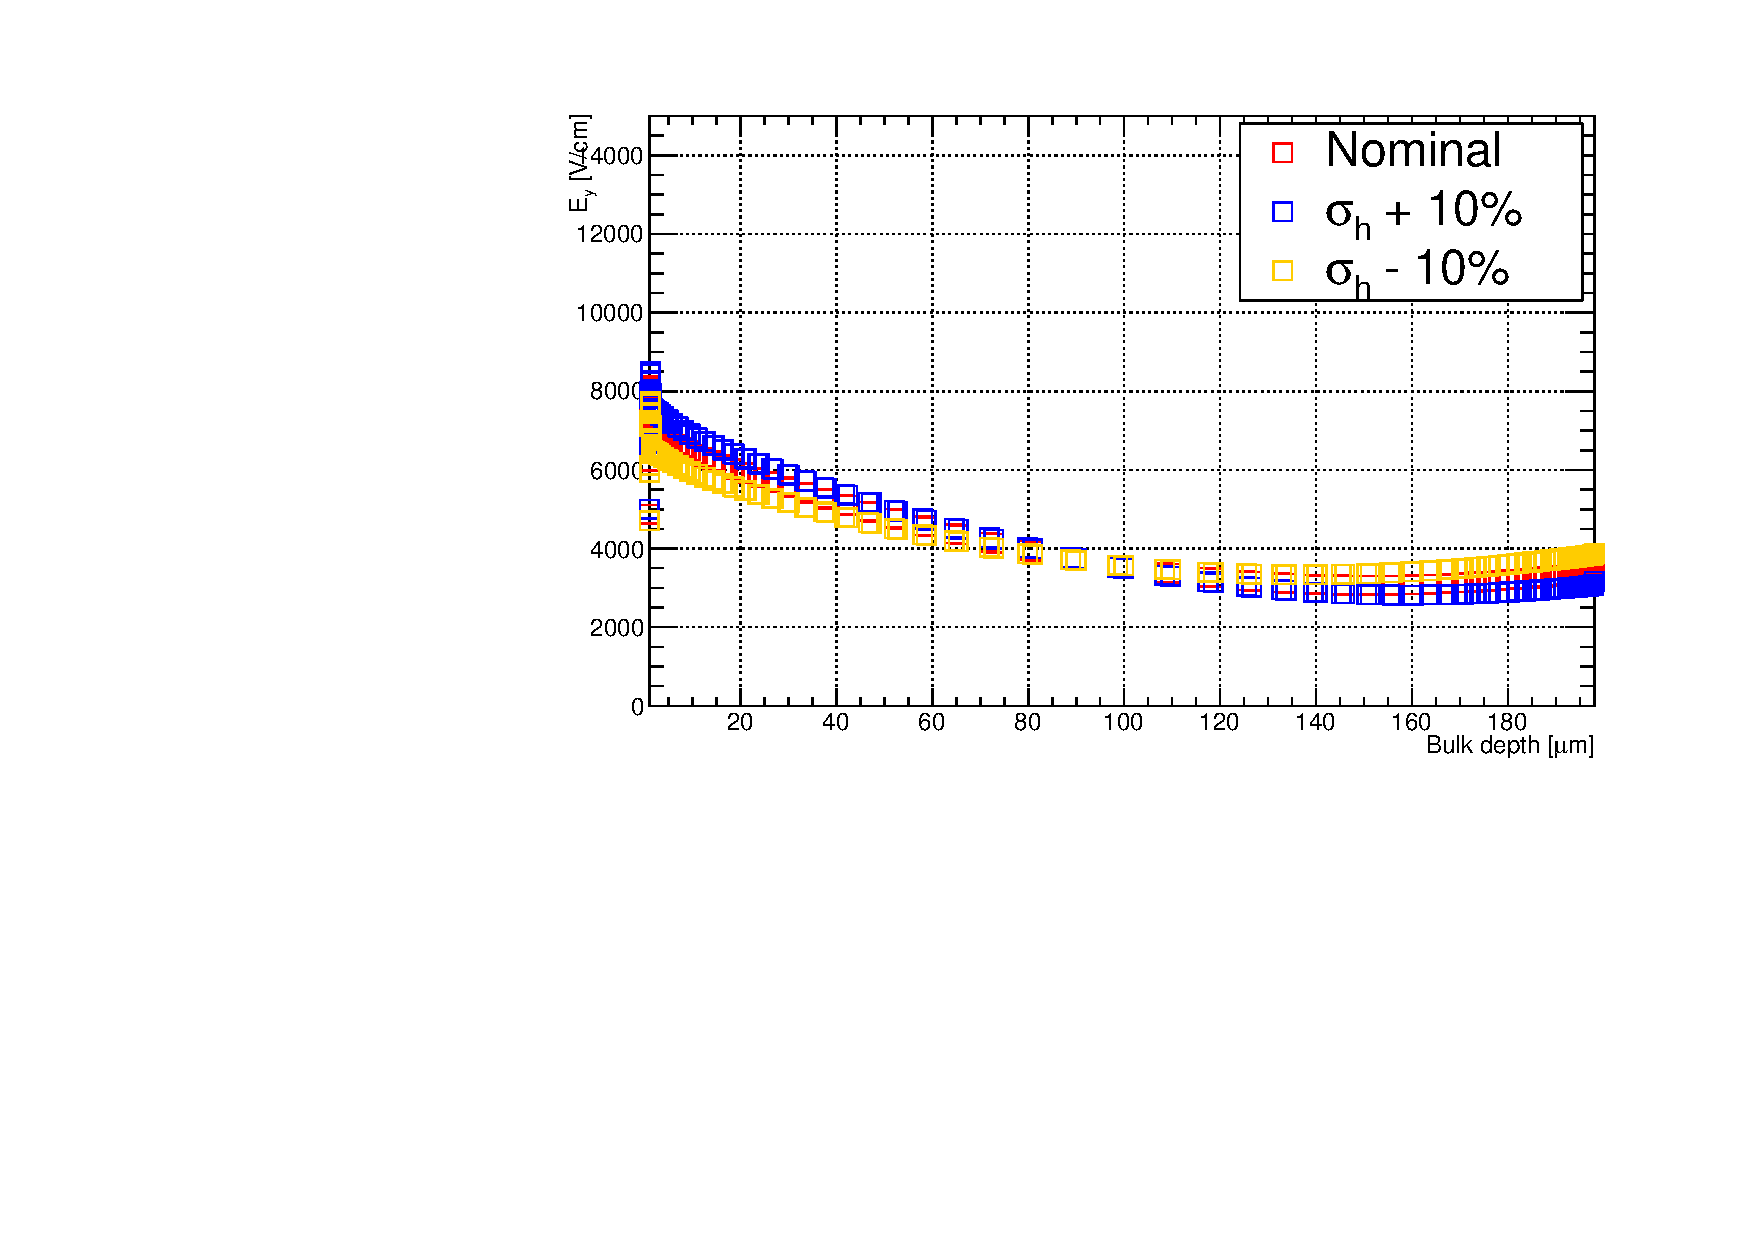
\includegraphics[width=0.49\textwidth]{new_Dsigmahvariation.pdf}
\caption{The $z$ dependence of the electric field in an ATLAS planar sensor, averaged over $x$ and $y$, for a simulated
  fluence of $\Phi=1\times10^{14}$~(1~MeV)~n$_\text{eq}/\text{cm}^{2}$, after varying parameters of the donor trap in the Chiochia model. (Top) The left plot shows a $\pm 10\%$ variation in the fluence dependence of the acceptor trap concentrations while the right plot shows a variation in the acceptor trap energy level by $0.4\%$. 
  (Bottom) The left plot shows a $\pm 10\%$ variation in the electron capture cross section, the right one a $\pm 10\%$ variation in the hole capture cross section.
The bias voltage was set to $80$ V in all cases.}
\label{fig:don_electricfieldvariations}
\end{figure}

It can be seen that the electric field profile is almost insensitive to the capture cross-sections, moderately sensitive to the fluence dependence of the trap concentrations ($\eta$), and highly sensitive to the energy level of the traps. 
Similar variations are observed when the trap concentrations are varied by $\pm10\%$ and the energy levels are varied by $\pm$ 10\% of the thermal voltage $V_{th}$ ($V_{th}=kT$), which corresponds roughly to $0.4\%$ of the energy level.  The latter number is chosen as a benchmark because the occupancy probability scales exponentially with the energy as $\sim e^{E/kT}$~\cite{LUTZ1996}; see also Appendix~\ref{sec:trapoccprob}. 
Interestingly, when the acceptor energy is moved closer to the conductive band by $0.4\%$, the electric field looks 
 symmetric around the mid-plane; moving the acceptor even closer to the conduction band would probably result in depletion 
 starting from the backside.
As expected, varying one parameter value for the acceptor trap has on the electric field an effect that is opposite 
to the one that is obtained when the same parameter is changed for the donor trap. 
All the observed changes in the electric field are consistent with expectations (see for example~\cite{LUTZ1996}).

The full charge collection efficiency from the model variations described in this section are presented in Appendix~\ref{sec:additional}.


\subsubsection{Effective modelling of annealing effects into TCAD simulations}
\label{sec:TCADAnneal} 
There is no known recipe to include the annealing effects presented in Section~\ref{sec:annealing} into 
TCAD based predictions.  One challenge for incorporating annealing effects is that both the Hamburg and TCAD models are based on multiple effective deep 
traps~\cite{bib:DP,CHIOCHIA2006} and the effective states are not exactly in one-to-one correspondence.  Furthermore, the Hamburg model does not make a prediction for the depth dependence of the effective doping concentration (Eq.~\ref{eq:hamburg13} assumes it is constant) while the TCAD model predicts a non-trivial dependence, resulting in the complicated electric field profile discussed in Sec.~\ref{sec:Efieldprofile}.  The non-constant charge density from TCAD is demonstrated in Fig.~\ref{fig:TCADSpaceCharge} for an ATLAS IBL planar sensor after radiation damage.   For $\Phi=1\times10^{14}$~(1~MeV)~n$_\text{eq}/\text{cm}^{2}$ the space charge 
density is negative and shows an almost linear dependence on the bulk depth, 
while for higher fluences the 
functional form is more complicated, exhibiting sizable regions where the charge density is positive, 
in agreement with the model first proposed in~\cite{bib:DP}.

\begin{figure}[!htpb]
\centering
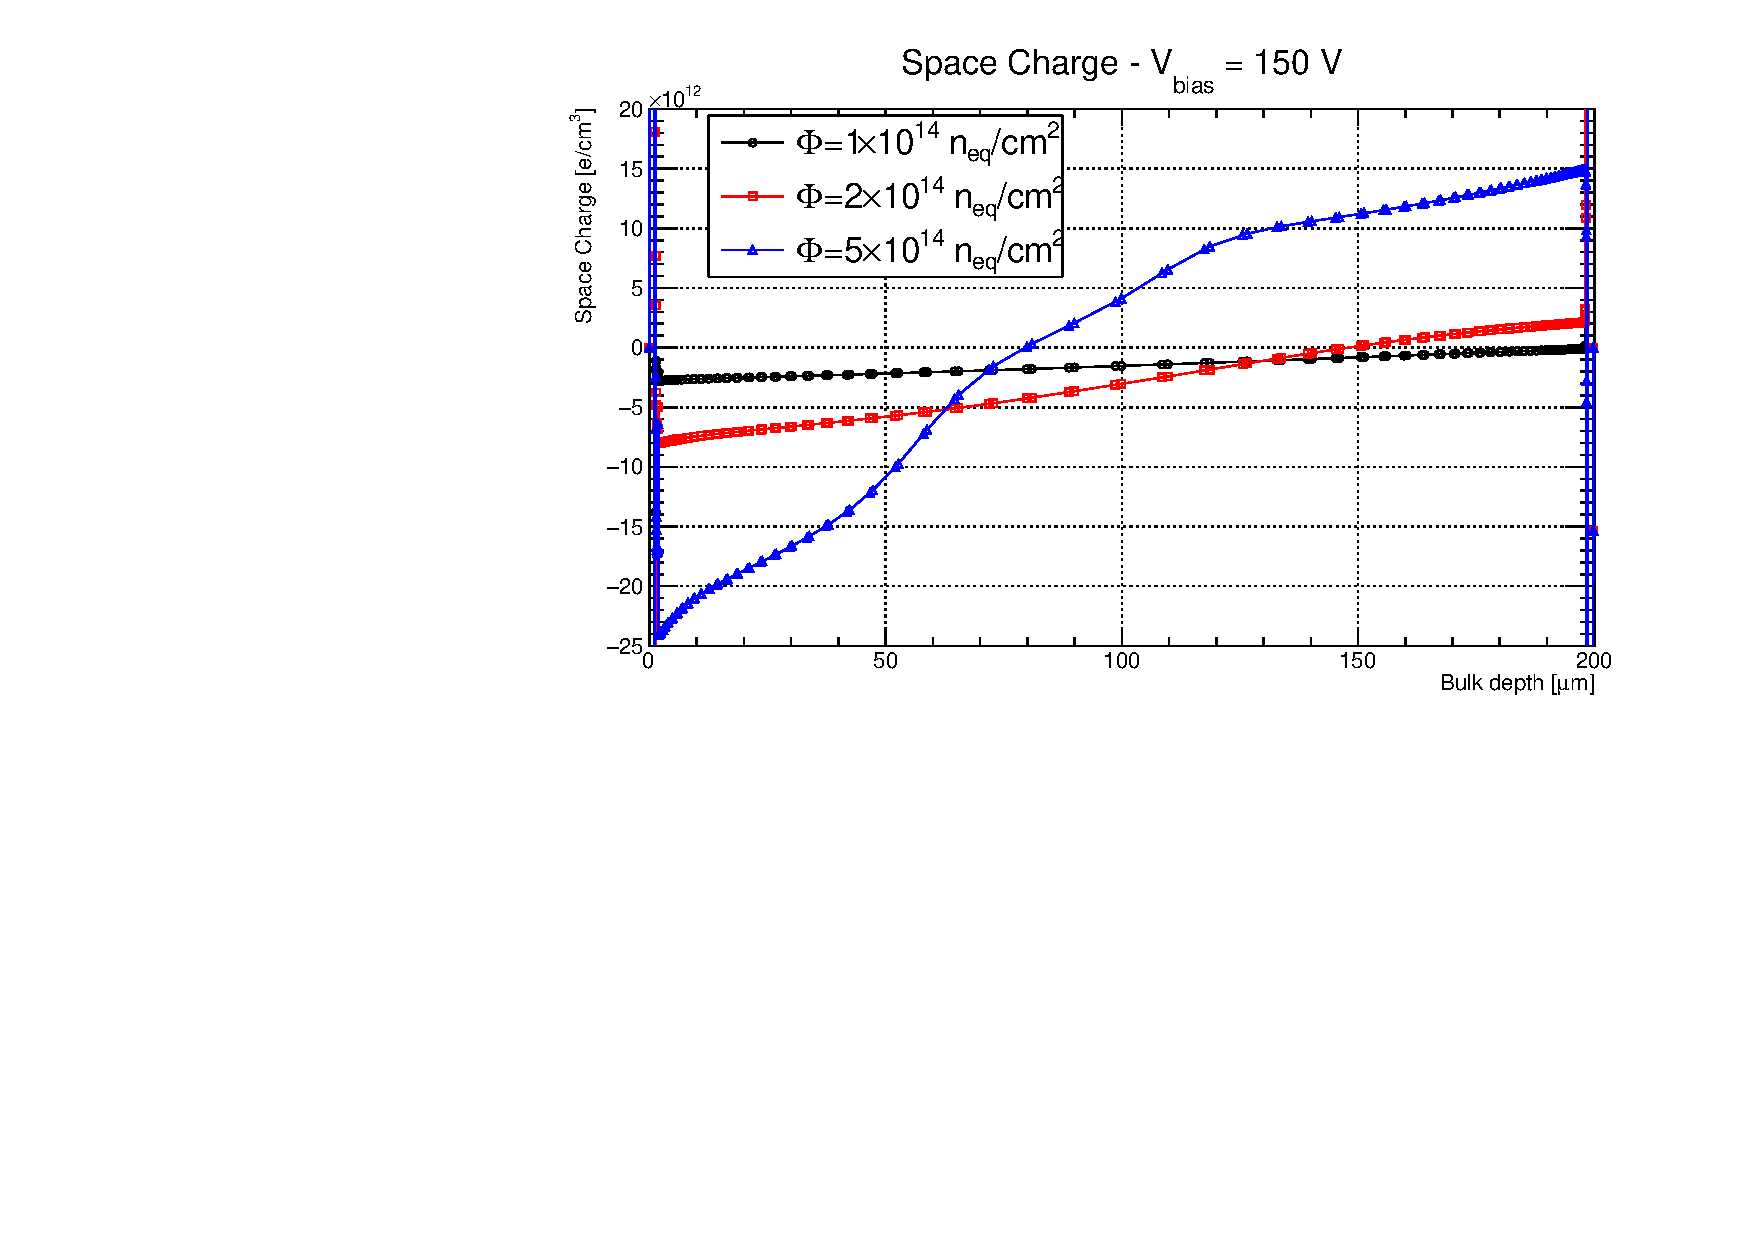
\includegraphics[width=0.6\textwidth]{TCAD_SpaceCharge_150V.pdf}
\caption{\label{fig:TCADSpaceCharge}The $z$ dependence of the normalised 
charge density $\rho/e$ in a simulated 
 ATLAS IBL planar sensor, averaged over $x$ and $y$, for  simulated
  fluences of $\Phi=1,\;2\; \text{and}\; 5\times10^{14}$~(1~MeV)~n$_\text{eq}/\text{cm}^{2}$. The bias voltage was set to $150$ V in all cases.}
\end{figure}

One way to emulate annealing effects from the Hamburg model in the TCAD simulation is to match the effective doping concentration from the former to the average charge density of the latter: 

\begin{equation}
\langle \rho/e\rangle_\text{TCAD}=(N_\text{eff})_\text{Hamburg}.
\label{eq:SpaceChargeTCADHamburg}
\end{equation}

Table~\ref{tab:NeffHamburg} collects predictions from the Hamburg model (see Sec.~\ref{sec:annealing}) for the effective concentration of donors and acceptors as well as their difference $N_\text{eff}$. 

\begin{table}[!htpb]
\centering
\begin{tabular}{|c|c|c|c|c|}
  \hline
   date & $\Phi$ [(1~MeV)~n$_\text{eq}/\text{cm}^{2}$] & $N_\text{eff}$ [cm$^{-3}$] 
   & $N_D$ [cm$^{-3}$]	& $N_A$ [cm$^{-3}$]	\\
   \hline	
  9/7/2016 & 1$\times10^{14}$ & 1.62$\times10^{12}$ & 0.08$\times10^{12}$ & 1.7$\times10^{12}$ \\
 8/9/2016 & 2$\times10^{14}$ & 2.72$\times10^{12}$ & 0.08$\times10^{12}$ & 2.8$\times10^{12}$\\
  \hline  
\end{tabular}
\caption{\label{tab:NeffHamburg}Predictions from the Hamburg model for the effective donor ($N_D$) and acceptor ($N_A$) concentrations as well as their difference ($N_\text{eff}$) for two point in time during Run 2.  Sec.~\ref{sec:annealing} for details.}
\end{table}

Figure~\ref{fig:NeffTCADAnnealing} shows the charge density predicted by TCAD simulations in four 
different scenarios with a bias voltage of 150~V and the two fluences reported in Table~\ref{tab:NeffHamburg}.  The \textit{Reference} scenario is the default setup described in Sec.~\ref{sec:ElectricField:SimulationDetails} with no modifications to emulate annealing.  Another extreme, labeled \textit{Annealed}, considers the acceptor and donor traps in the Hamburg model TCAD as in one-to-one correspondence.  Therefore, instead of matching the effective doping concentration as in Eq.~\ref{eq:SpaceChargeTCADHamburg}, the acceptor and donor densities in TCAD are directly set to the values in Table~\ref{tab:NeffHamburg}.  Moreover, since shallow defects are not affected by deep traps in TCAD, the way to account for the fact that in Hamburg model the shallow donors are supposed to be completely annealed out is to reduce significantly the initial concentration of shallow donors. So, additionally, the doping level in the starting material is set to 8$\times$10$^{10}$~cm$^{-3}$;  as a reminder the initial donor concentration was of about 1.6$\times$10$^{12}$~cm$^{-3}$.   The Annealed scenario is qualitatively different than the un-annealed line and would predict an electric field that is linear (more below), which is in contrast to various measurements elsewhere~\cite{CHIOCHIA2006} and also shown later in this paper (Sec.~\ref{sec:CCE}).  Therefore, a compromise is made in which only the average effective doping concentration is matched between the models, following Eq.~\ref{eq:SpaceChargeTCADHamburg}.  There is some freedom in how to do the matching because donors and acceptors can be independently varied.  For high fluences 
($\gtrsim10^{13}$~(1~MeV)~n$_\text{eq}/\text{cm}^{2}$), deep and shallow donor states are more likely than acceptors to be completely removed~\cite{moll-thesis}.  Therefore, we vary only the acceptor concentrations when solving Eq.~\ref{eq:SpaceChargeTCADHamburg}.   The values that match the Hamburg model are $+3\%$ for $\Phi=1\times10^{14}$ $n_\text{eq}/\text{cm}^2$ and $-1.6\%$ for $\Phi=2\times10^{14}$ $n_\text{eq}/\text{cm}^2$.  For reference, the space charge distributions for $+10\%$ and $-5\%$ for the two fluences are also shown, respectively.   The average charge density in the various scenarios is summarized In Table~\ref{tab:TCADNeffHamburg1}~and~\ref{tab:TCADNeffHamburg2} for the two fluences shown in Fig.~\ref{fig:NeffTCADAnnealing}.

\begin{figure}[!htpb]
\centering
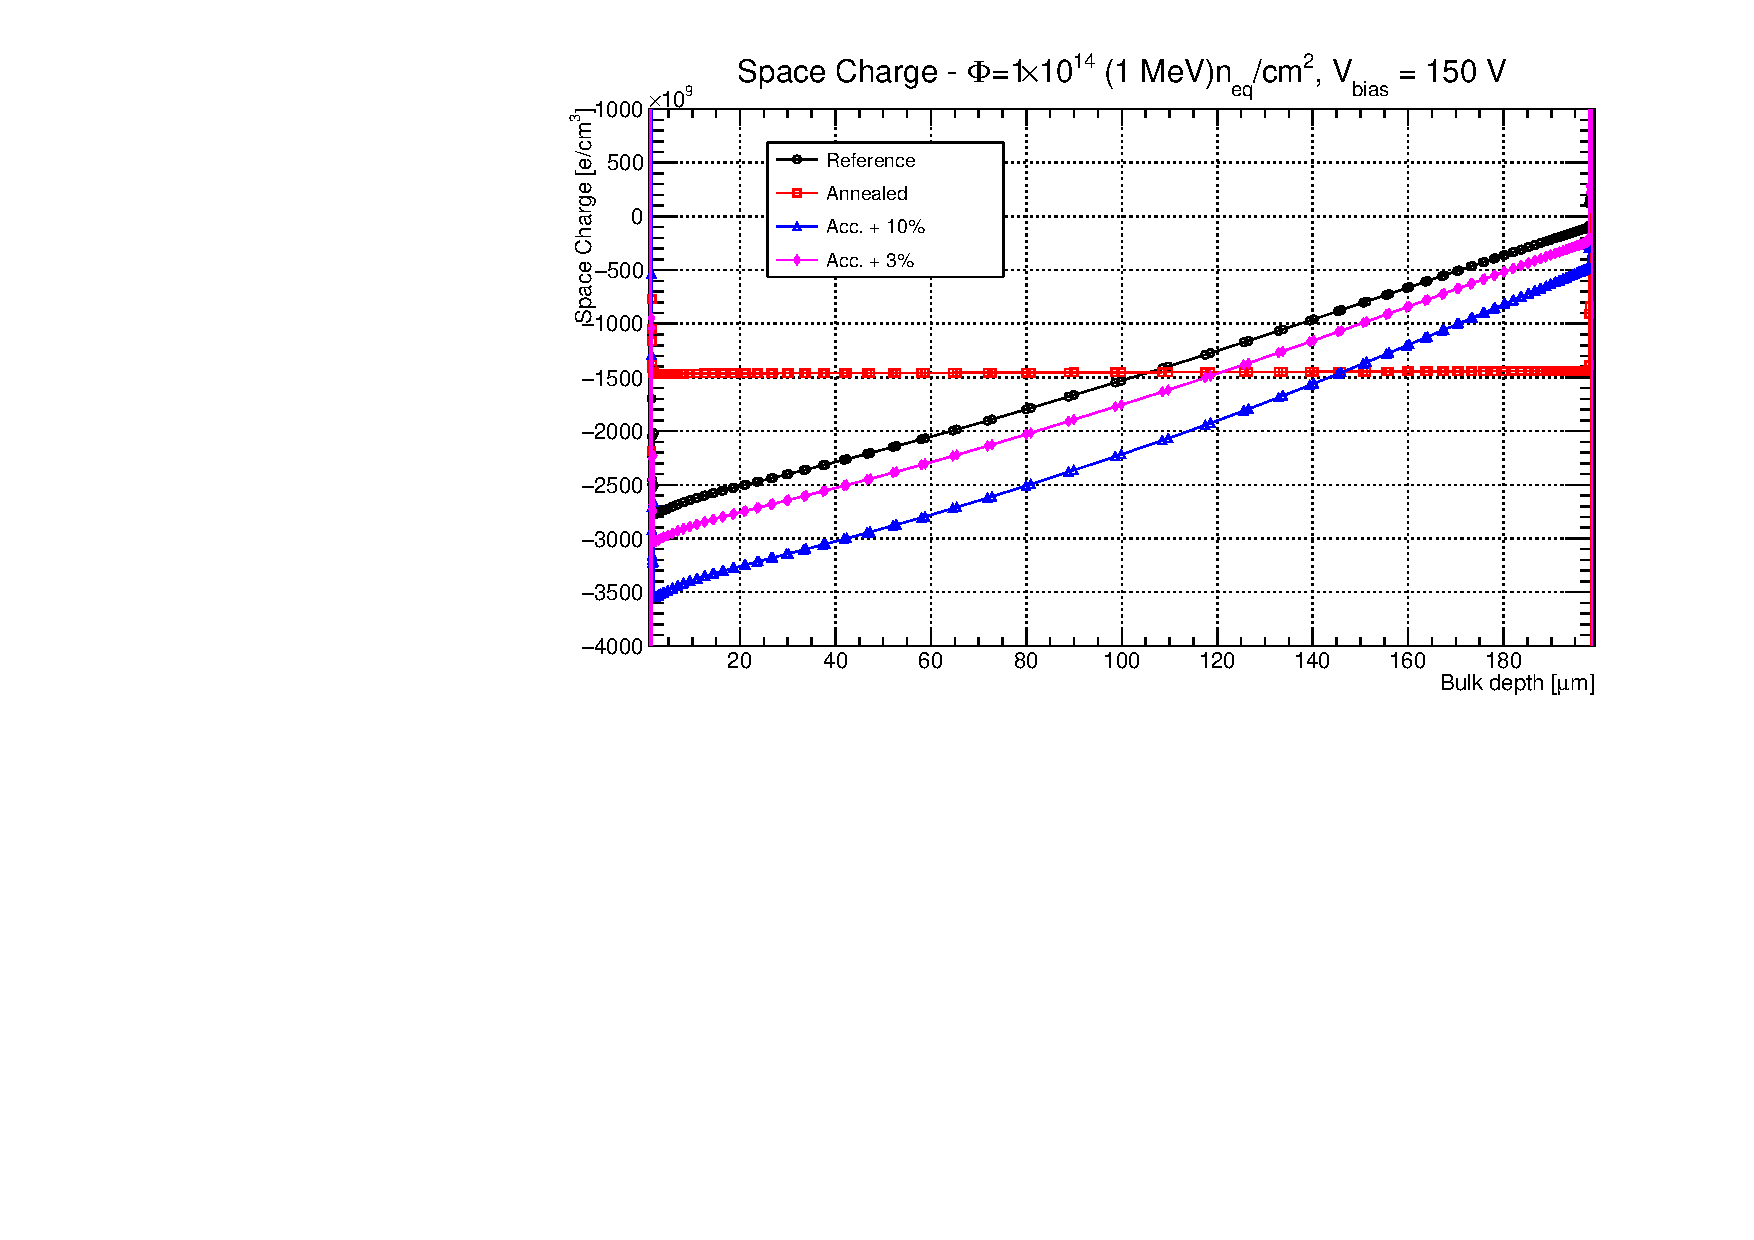
\includegraphics[width=0.49\textwidth]{TCAD_SpaceCharge_variations_1e14_150V.pdf}
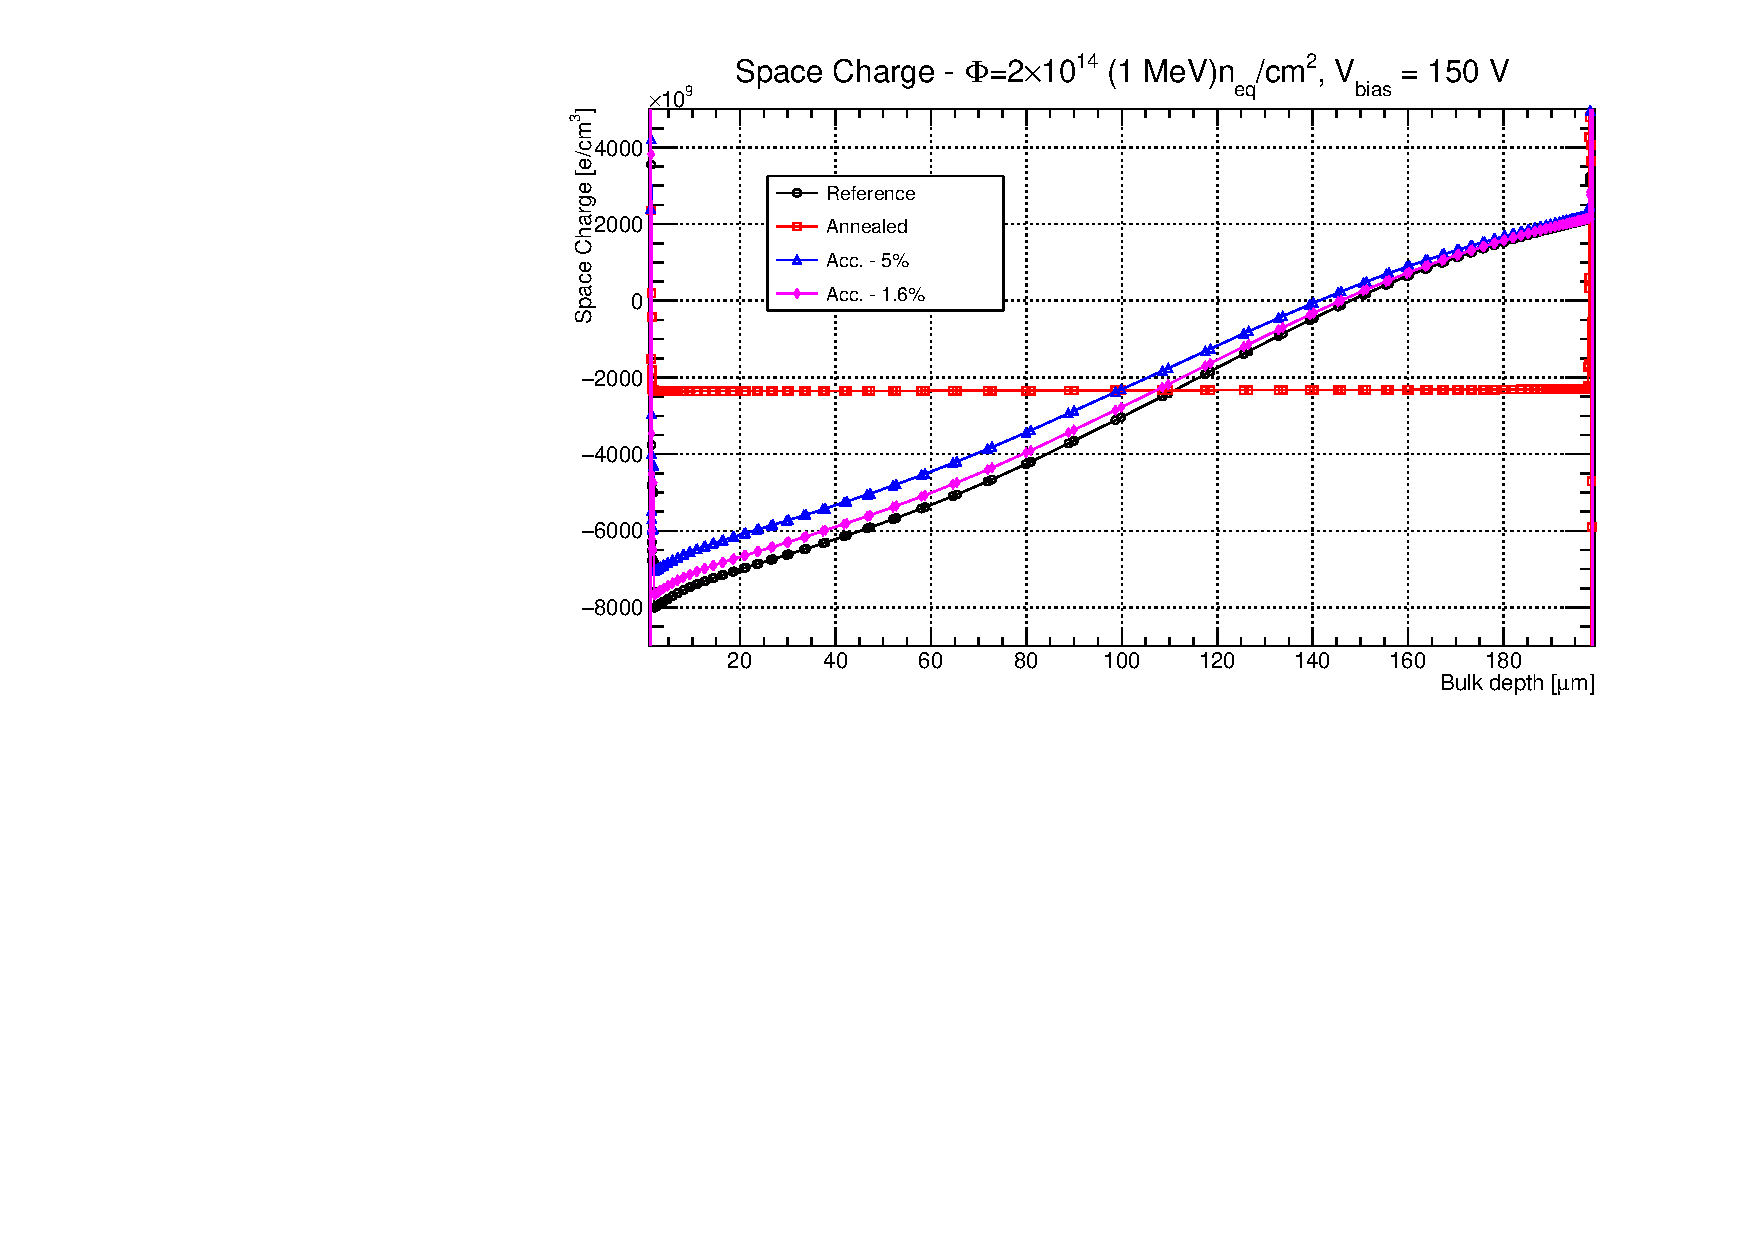
\includegraphics[width=0.49\textwidth]{TCAD_SpaceCharge_variations_2e14_150V.pdf}
\caption{\label{fig:NeffTCADAnnealing}The $z$ dependence of the normalised charge density $\rho/e$ in a simulated ATLAS IBL planar sensor, averaged over $x$ and $y$, for  simulated
  fluences of (left)~$\Phi=1$~and~(right)~2$\times10^{14}$~(1~MeV)~n$_\text{eq}/\text{cm}^{2}$. The bias voltage was set to $150$ V in all cases. Four scenarios were simulated; see text for more 
  details.}
\end{figure}


\begin{table}[htbp]
   \centering
   \begin{tabular}{|c|c|c|} 
      \hline
            \multicolumn{3}{|c|}{$\Phi=1\times10^{14}$~(1~MeV)~n$_\text{eq}/\text{cm}^{2}$  } \\
      \hline 
        Scenario  & $\langle N_\text{eff}\rangle$ [cm$^{-3}$] & RMS [cm$^{-3}$] \\
      \hline
       Reference &  -1.5$\times10^{12}$ & 0.4$\times10^{12}$  \\
 Annealed   & -1.45$\times10^{12}$ & 0.04$\times10^{12}$ \\
 $N_A$+10\% &  -2.2$\times10^{12}$ & 0.6$\times10^{12}$  \\
 $N_A$+3\% &  -1.7$\times10^{12}$ & 0.5$\times10^{12}$  \\
      \hline
         \end{tabular}
   \caption{\label{tab:TCADNeffHamburg1}Results for average and RMS of effective doping concentration over the sensor bulk from TCAD simulation for different scenarios. 
Fluence $\Phi$ was 1$\times10^{14}$~(1~MeV)~n$_\text{eq}/\text{cm}^{2}$; bias voltage $V_\text{bias}$ 
was 150~V.  Refer to the text for more details.}
\end{table}




% Requires the booktabs if the memoir class is not being used
\begin{table}[htbp]
   \centering
   %\topcaption{Table captions are better up top} % requires the topcapt package
   \begin{tabular}{|c|c|c|} % Column formatting, @{} suppresses leading/trailing space
      \hline
            \multicolumn{3}{|c|}{$\Phi=2\times10^{14}$~(1~MeV)~n$_\text{eq}/\text{cm}^{2}$  } \\
      \hline % Partial rule. (r) trims the line a little bit on the right; (l) & (lr) also possible
        Scenario  & $\langle N_\text{eff}\rangle$ [cm$^{-3}$] & RMS [cm$^{-3}$] \\
      \hline
         Reference &  -2.9$\times10^{12}$ & 2.1$\times10^{12}$  \\
 Annealed   & -2.34$\times10^{12}$ & 0.01$\times10^{12}$ \\
 $N_A$-5\% &  -2.3$\times10^{12}$ & 2.8$\times10^{12}$  \\
 $N_A$-1.6\% &  -2.7$\times10^{12}$ & 2.1$\times10^{12}$  \\
                   \bottomrule
   \end{tabular}
   \caption{\label{tab:TCADNeffHamburg2}Results for average and RMS of effective doping concentration over the sensor bulk from TCAD simulation for different scenarios. 
Fluence $\Phi$ was 2$\times10^{14}$~(1~MeV)~n$_\text{eq}/\text{cm}^{2}$; bias voltage $V_\text{bias}$ 
was 150~V.  Refer to the text for more details.}
\end{table}

The electric field profiles corresponding to the four scenarios shown in Fig.~\ref{fig:NeffTCADAnnealing} are presented in Fig.~\ref{fig:EFieldTCADAnnealing} the corresponding simulated electric field profiles for the 
same scenarios are presented.   For the Annealed scenario (shown only for reference), the profile is nearly linear while this is not the case for the other scenarios, especially at the higher fluence $\Phi=2\times10^{14}$~(1~MeV)~n$_\text{eq}/\text{cm}^{2}$.  


\begin{figure}[!htpb]
\centering
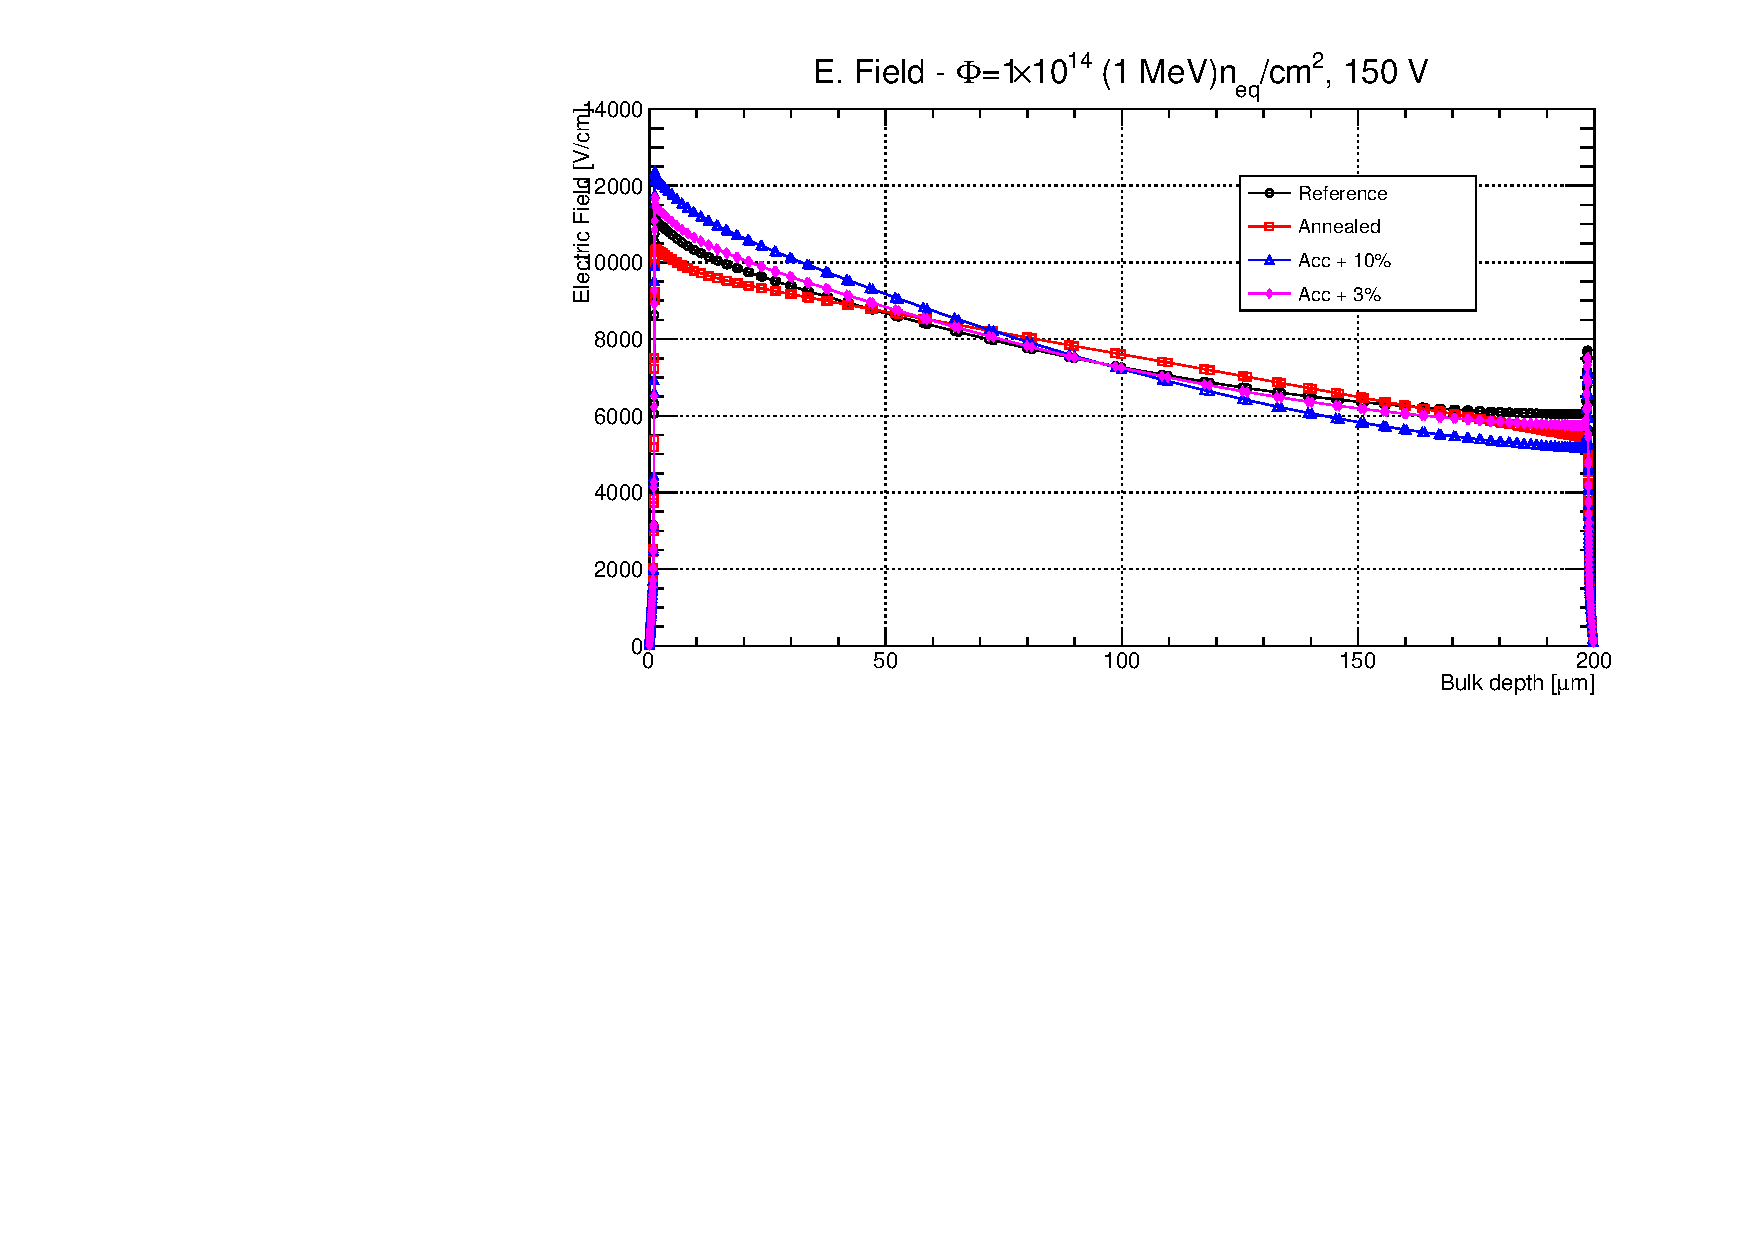
\includegraphics[width=0.49\textwidth]{TCAD_EField_variations_1e14_150V.pdf}
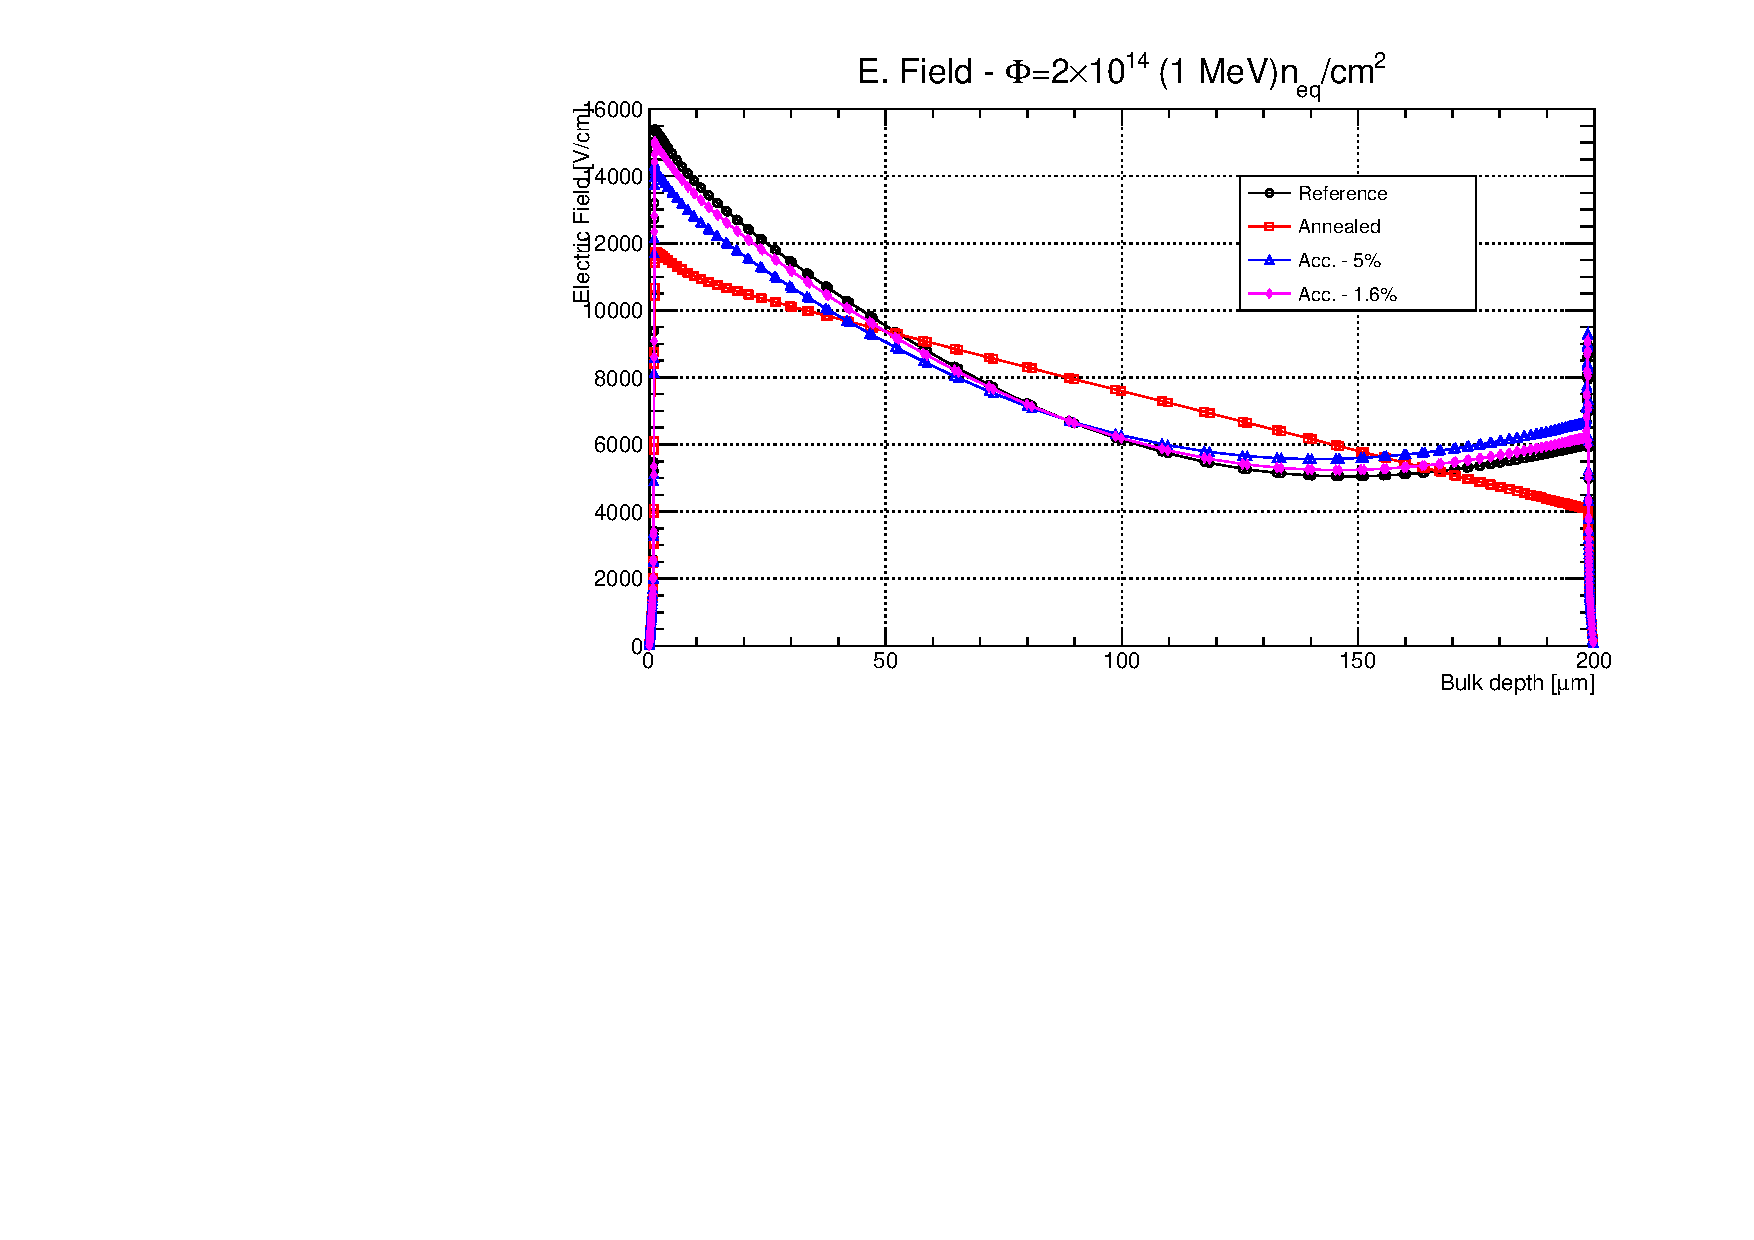
\includegraphics[width=0.49\textwidth]{TCAD_EField_variations_2e14_150V.pdf}
\caption{\label{fig:EFieldTCADAnnealing}The $z$ dependence of the electric field in a simulated ATLAS IBL planar sensor, averaged over $x$ and $y$, for  simulated
  fluences of (left)~$\Phi=1$~and~(right)~2$\times10^{14}$~(1~MeV)~n$_\text{eq}/\text{cm}^{2}$. The
bias voltage was set to $150$ V in all cases. Four scenarios were simulated; see text for more 
  details.}
\end{figure}

In summary, increasing the acceptor traps density by 3\% at fluence 
$\Phi=1\times10^{14}$~(1~MeV)~n$_\text{eq}/\text{cm}^{2}$, and reducing it by 1.6\% 
at fluence $\Phi=2\times10^{14}$~(1~MeV)~n$_\text{eq}/\text{cm}^{2}$ the effect of annealing 
predicted by Hamburg model can be emulated with the TCAD simulations.   These variations are currently within the model variations described in Sec.~\ref{sec:Efieldmodelcomparisons} that are used to set systematic uncertainties on the radiation damage model parameters.  Therefore, no additional corrections or uncertainties are applied to the simulation to account for annealing for the current radiation levels.


\subsection{Time-to-electrode, Location-at-trap}
\label{sec:maps}

Numerically propagating charges through the silicon sensor can be computationally expensive, but fortunately can be computed once per geometry and set of conditions (temperature, bias, and fluence).   Electrons and holes drift with a velocity given by the mobility: $\mu_C$, where $C\in\{e,h\}$.  The mobility is parameterized as a function of electric field and temperature~\cite{JACOBONI197777}:

\begin{align}
\label{eq:mobility}
\mu_{C}(E)\approx \frac{v_{s,C}}{E_{c,C}}\left(1+\left(\frac{E}{E_{\text{crit},C}}\right)^{\beta_C}\right)^{-1/{\beta_C}},
\end{align}

\noindent where the values for the saturation velocity $v_s$, critical $E$-field $E_\text{crit}$ and temperature exponent $\beta$ can be found in Table~\ref{eq:constants_rad}.  Importantly, the saturation velocity for electrons is much higher than for holes.  The magnetic field modifies the mobility by the Hall scattering factor $r$ by $\mu\mapsto r\mu$, with the temperature-dependent $r$ given in Table~\ref{eq:constants_rad}.  Fundamental charge carriers drift with a velocity given by $v(E)\sim r\mu(E)E$ and the charge collection time is estimated via

\begin{align}
\label{eq:timetoelectrode}
t_\text{collection}(\vec{x}_\text{initial})\sim\int_\text{$\vec{x}_\text{initial}$}^\text{$\vec{x}_\text{final}$}\frac{ds}{r\mu(E)E},
\end{align}

where $s$ is determined by the equations of motion $\vec{v}=r\mu(E)\vec{E}$ and $\vec{x}_\text{final}$ depends on the type of the charge carrier.  For planar sensors, the field is nearly independent of $x$ and $y$, so the time to the electrode is parameterized in $z$ and the integral in Eq.~\ref{eq:timetoelectrode} is one-dimensional.  In contrast, for 3D sensors, the field depends strongly on $x$ and $y$, but is mostly independent of $z$.  Therefore, $t_\text{collection}(\vec{x}_\text{initial})$ is represented as a two-dimensional map.  Representative time-to-electrode maps are shown in Figs~\ref{fig:timetoelectrode} and~\ref{fig:timetoelectrode3D} for planar and 3D sensors, respectively.  Since the mobility of holes is much less than for electrons, it takes holes much longer on average to fully drift.  The collection time varies with fluence, bias voltage, and distance to the electrode, but is on average $\mathcal{O}(1)$-$\mathcal{O}(10)$ ns for $\Phi\lesssim 10^{15}$ $n_\text{eq}/\text{cm}^2$.

\begin{figure}[!htpb]
\centering
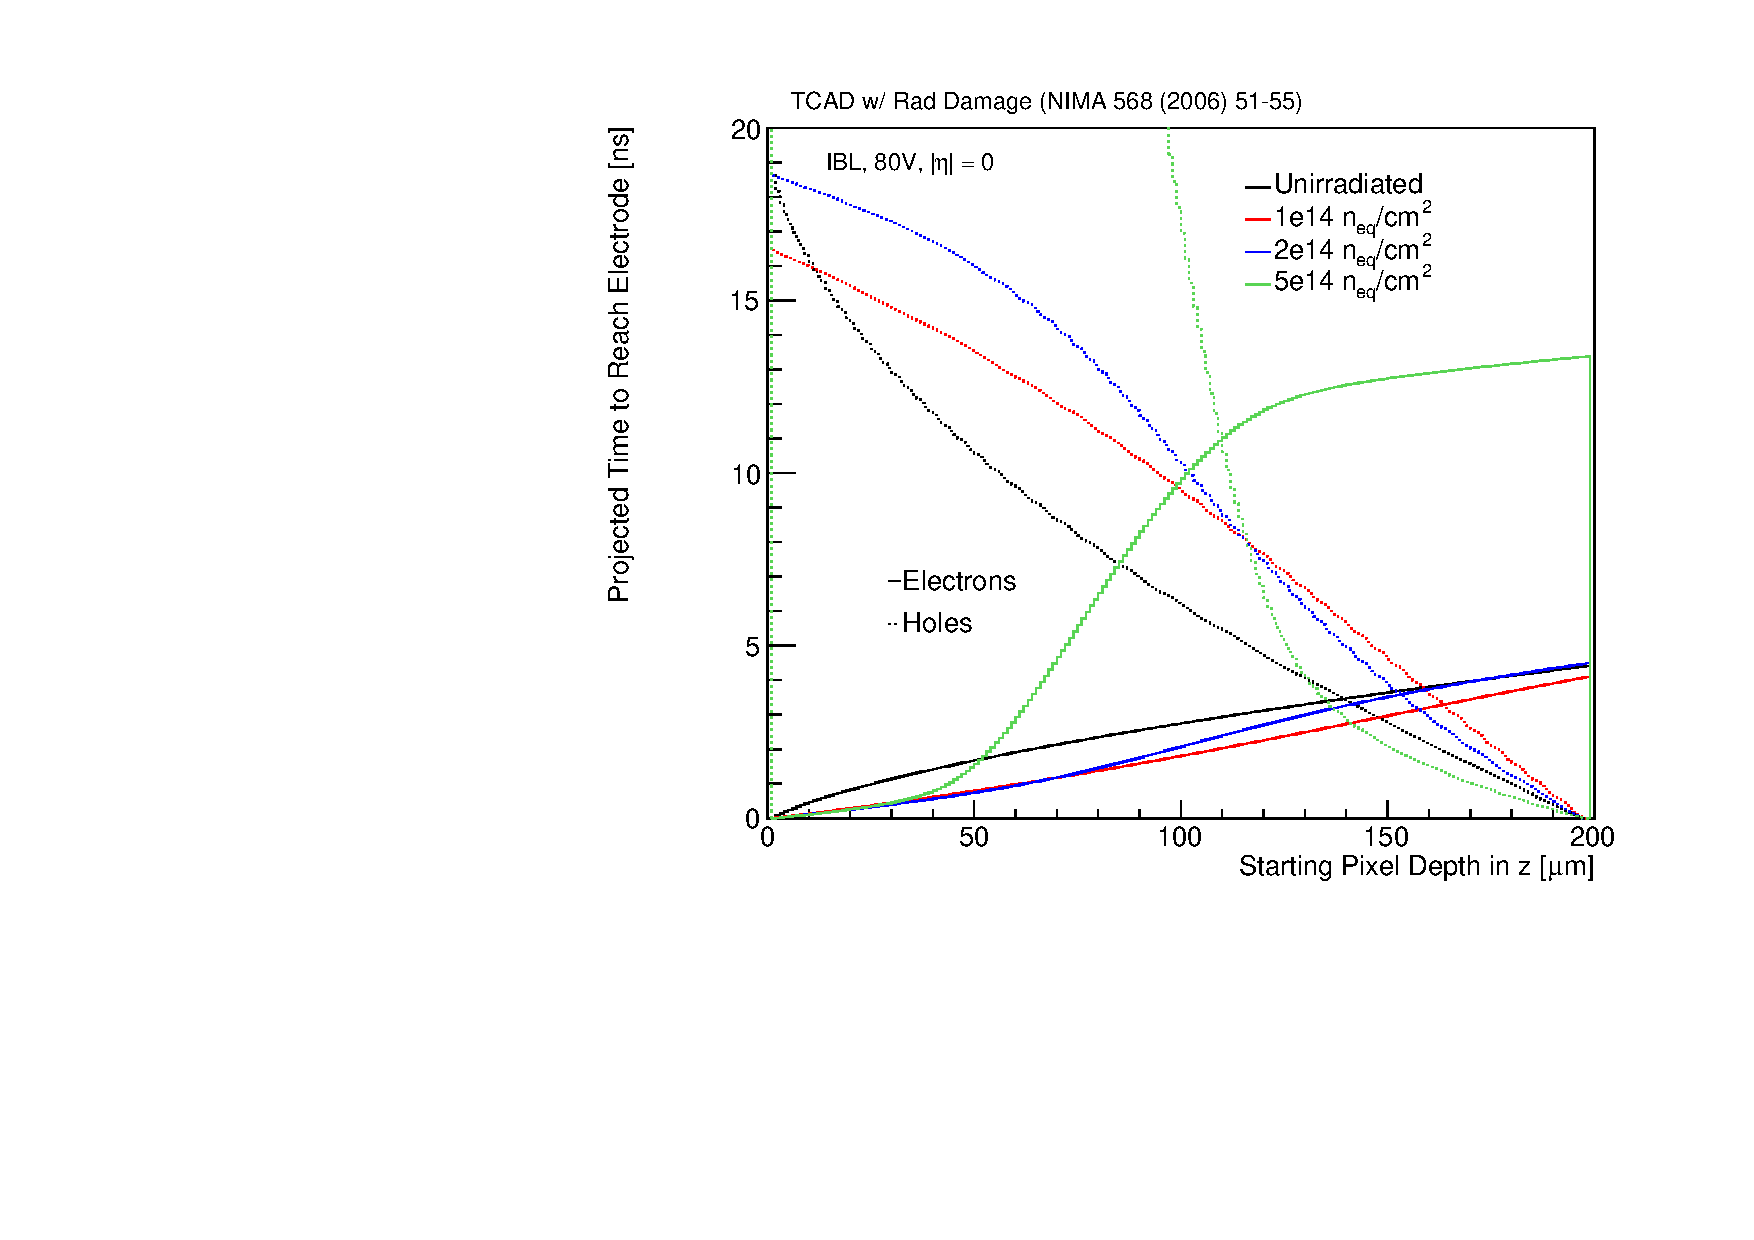
\includegraphics[width=0.6\textwidth]{tz_0fluence80V.pdf}
\caption{The time for an electron or hole to drift all the way to the collecting electrode (electrons) or back plane (holes) in an ATLAS IBL planar sensor biased at 80 V as a function of the depth ($z$) using the averaged $E$ fields shown in Fig.~\ref{fig:electricfield:profilesRun23}.  }
\label{fig:timetoelectrode}
\end{figure}

\begin{figure}[!htpb]
\centering
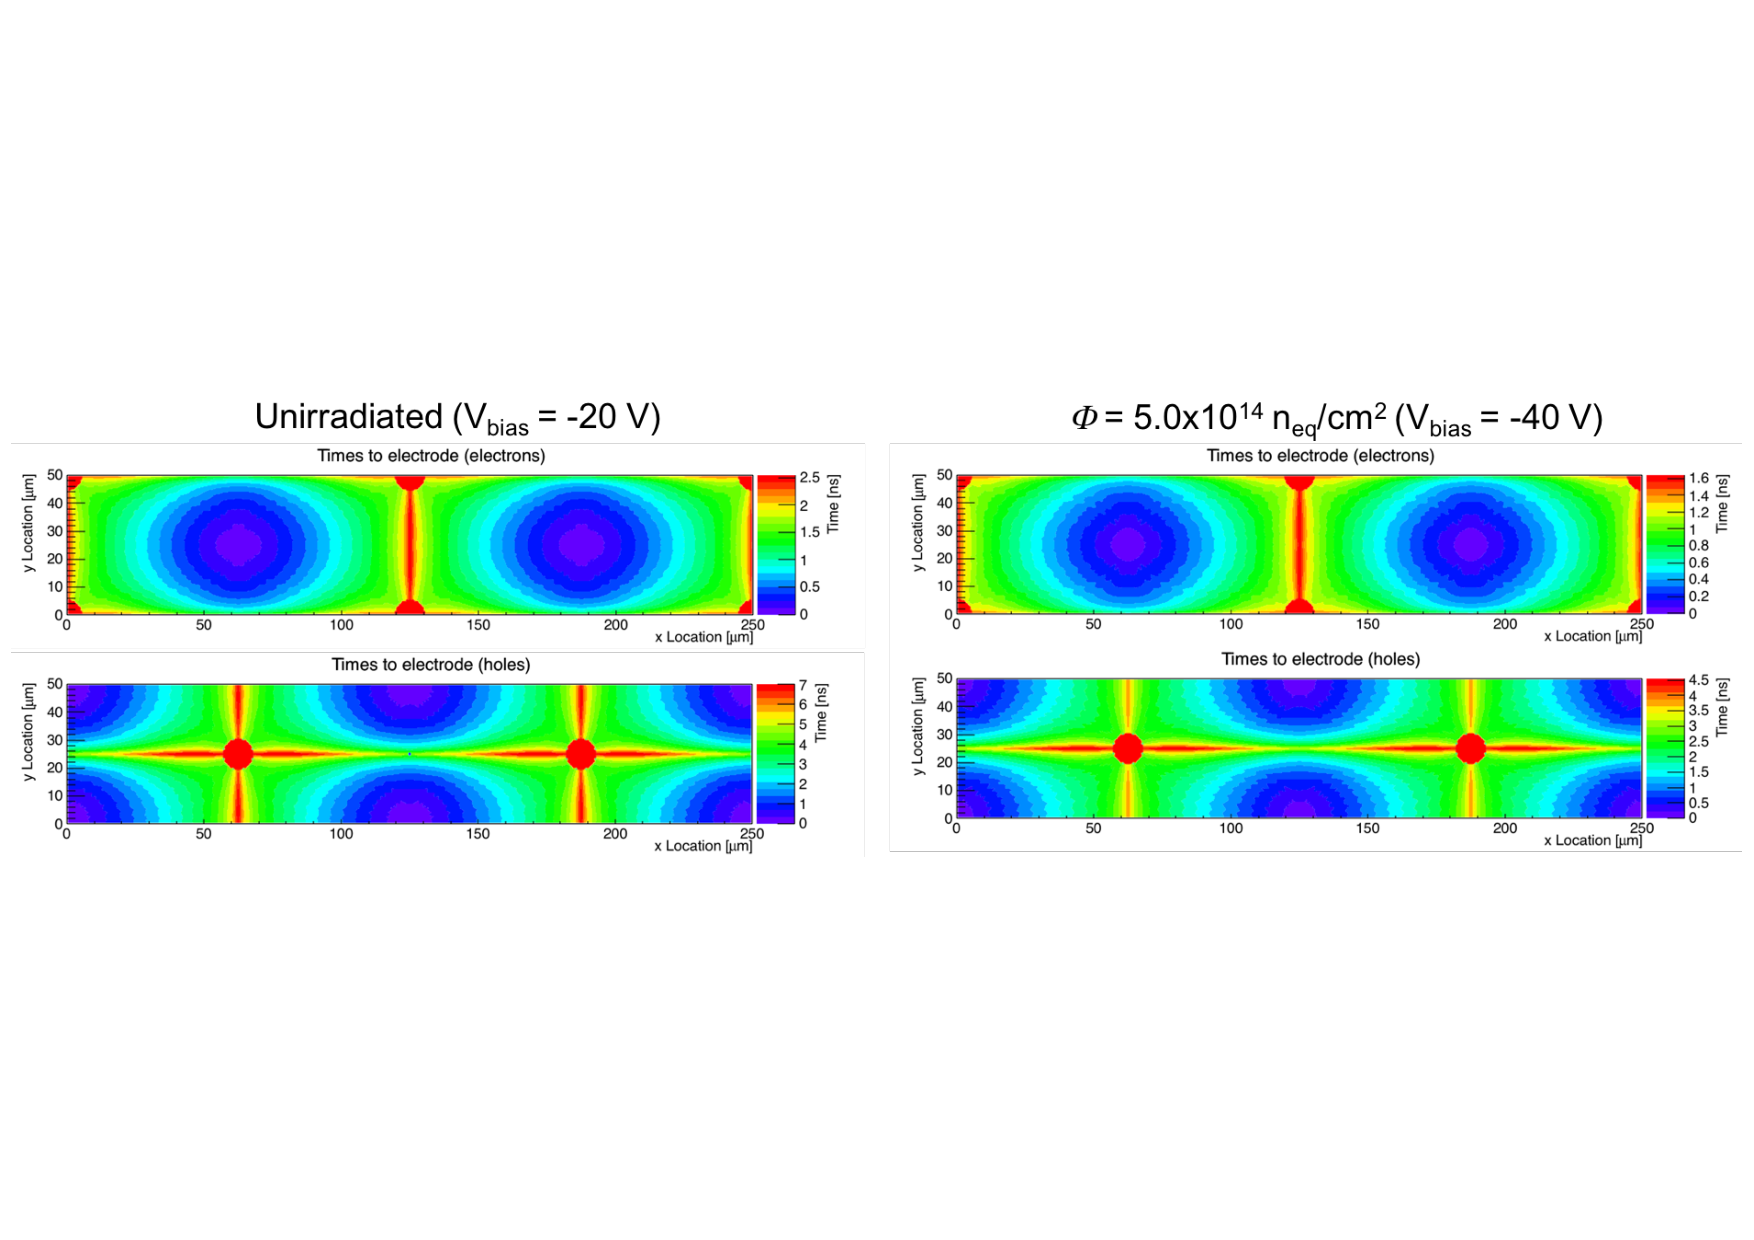
\includegraphics[width=0.95\textwidth]{Figure10.pdf}
\caption{Top (bottom): The time for an electron or hole to drift all the way to the $n^+$ electrode (electrons) or $p^+$ electrode (holes) for an ATLAS IBL 3D sensor.  The maps on the left are computed for unirradiated sensors, while those on the right have a fluence of $5\times 10^{14}$ $n_\text{eq}/\text{cm}^2$.  }
\label{fig:timetoelectrode3D}
\end{figure}

\begin{table}[!htpb]
\centering
\begin{tabular}{|c|c|c|}
  \hline
   quantity & electrons & holes		\\
   \hline	
  $v_s$ ($\mu$m/ns) & $116\times (T/273\text{ K})^{-0.87}$ & $88\times (T/273\text{ K})^{-0.52}$ \\
  $E_\text{crit}$ (kV/cm) & $6.0 \times (T/273\text{ K})^{1.55}$ & $15 \times  (T/273\text{ K})^{1.68}$ \\
  $\beta$ & $1.0 \times (T/273\text{ K})^{0.66} $& $1.1\times (T/273\text{ K})^{0.17} $\\
  $r$ &$1.13+8\times 10^{-4}\times (T/\text{K}-273)$ & $0.72-5\times 10^{-4}\times (T/\text{K}-273)$\\
  \hline  
\end{tabular}
\caption{Physical constants describing the mobility of charge carriers in silicon.  The first three rows are reformatted from Ref.~\cite{JACOBONI197777} and the Hall scale factor is from Ref.~\cite{hall1}.}
\label{eq:constants_rad}
\end{table}

For charges that are trapped (see Sec.~\ref{sec:chargetrapping}), one must know the location of the trapped charge.  The position-at-trap can be calculated in a similar fashion as the time-to-electrode from Eq.~\ref{eq:timetoelectrode}.  In particular, 

\begin{align}
\label{eq:traptimetoelectrode}
\vec{x}_\text{trap}(t_\text{to trap})\sim\int_\text{$0$}^\text{$t_\text{to trap}$}r\mu(E)\vec{E}dt.
\end{align}

\noindent Representative position-at-trap maps are shown in Fig.~\ref{fig:posattrap} for planar sensors.  The corresponding 3D maps are more difficult to visualize due to its high dimensionality.

\begin{figure}[!htpb]
\centering
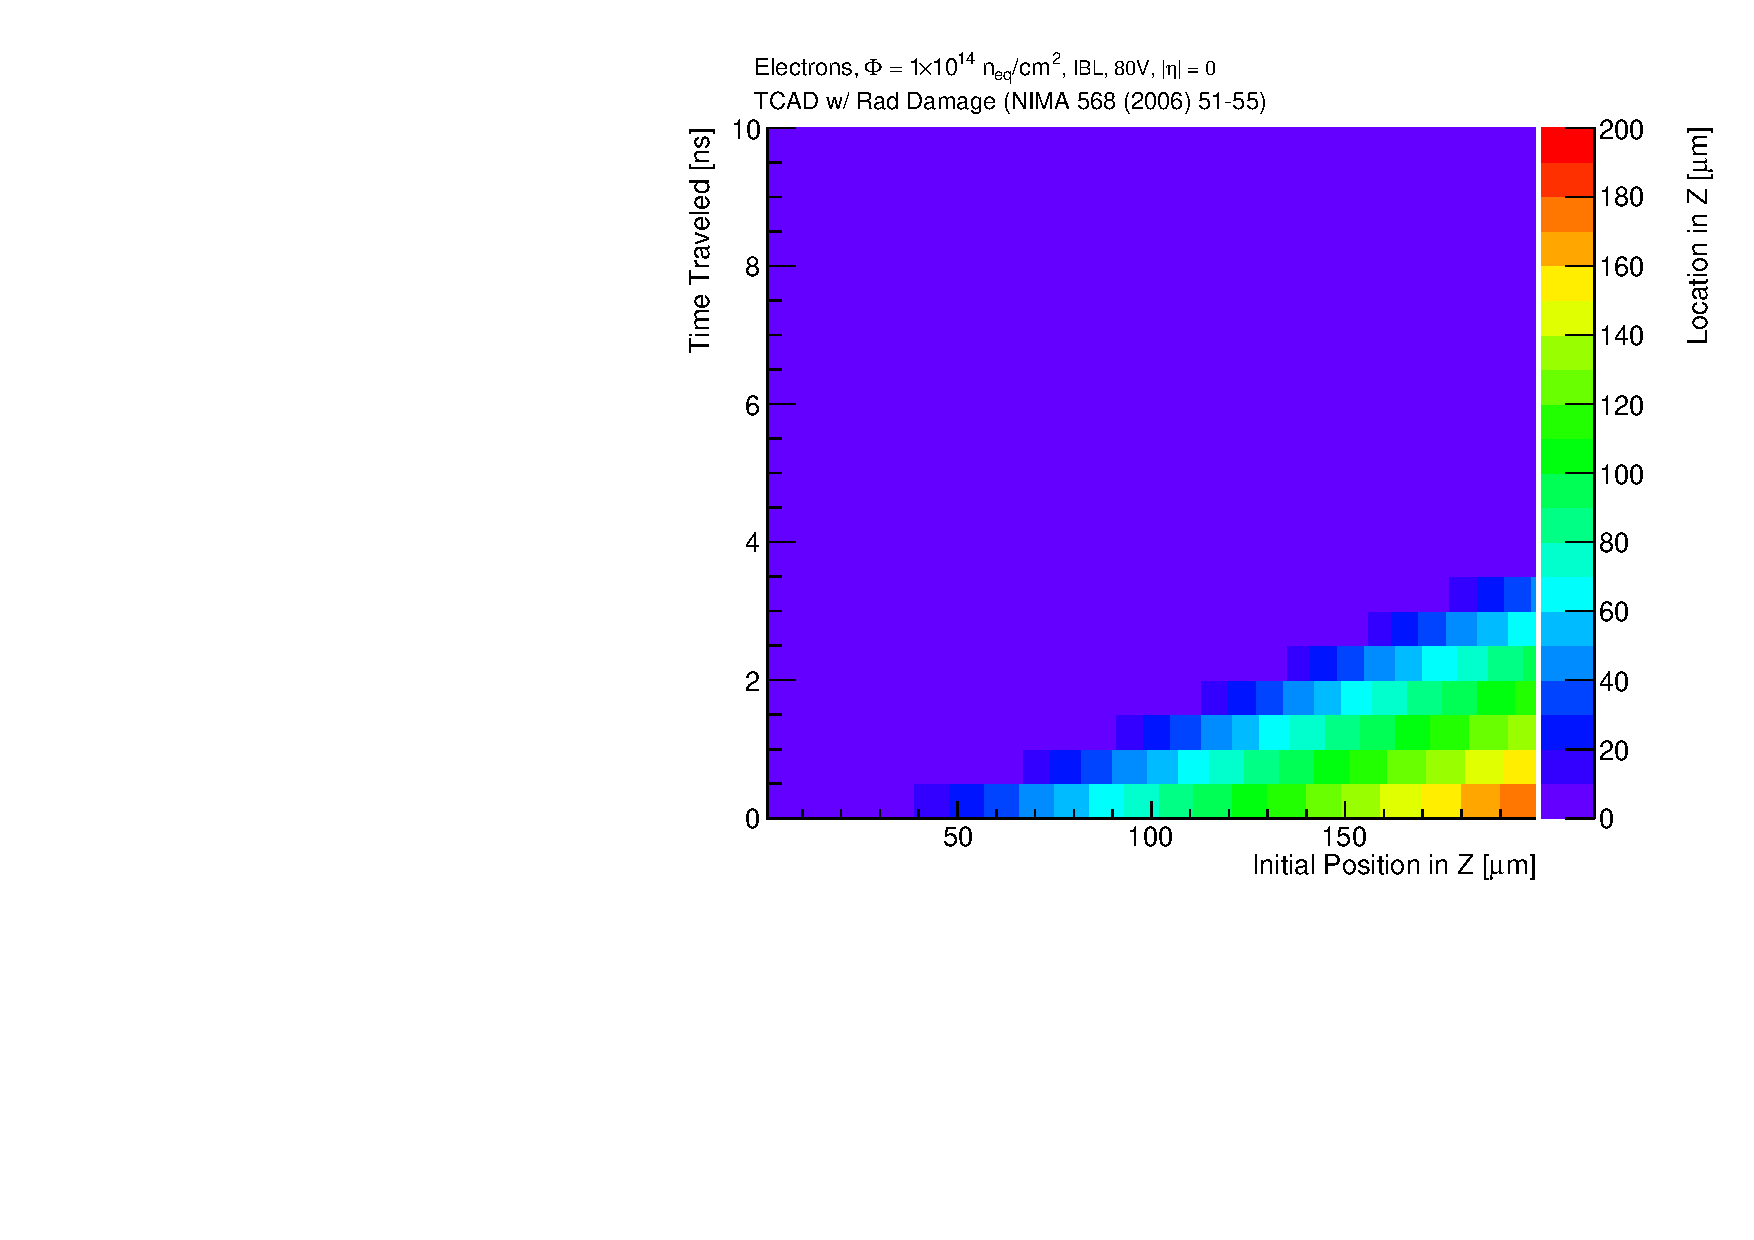
\includegraphics[width=0.49\textwidth]{distance_maps_e1e14.pdf}
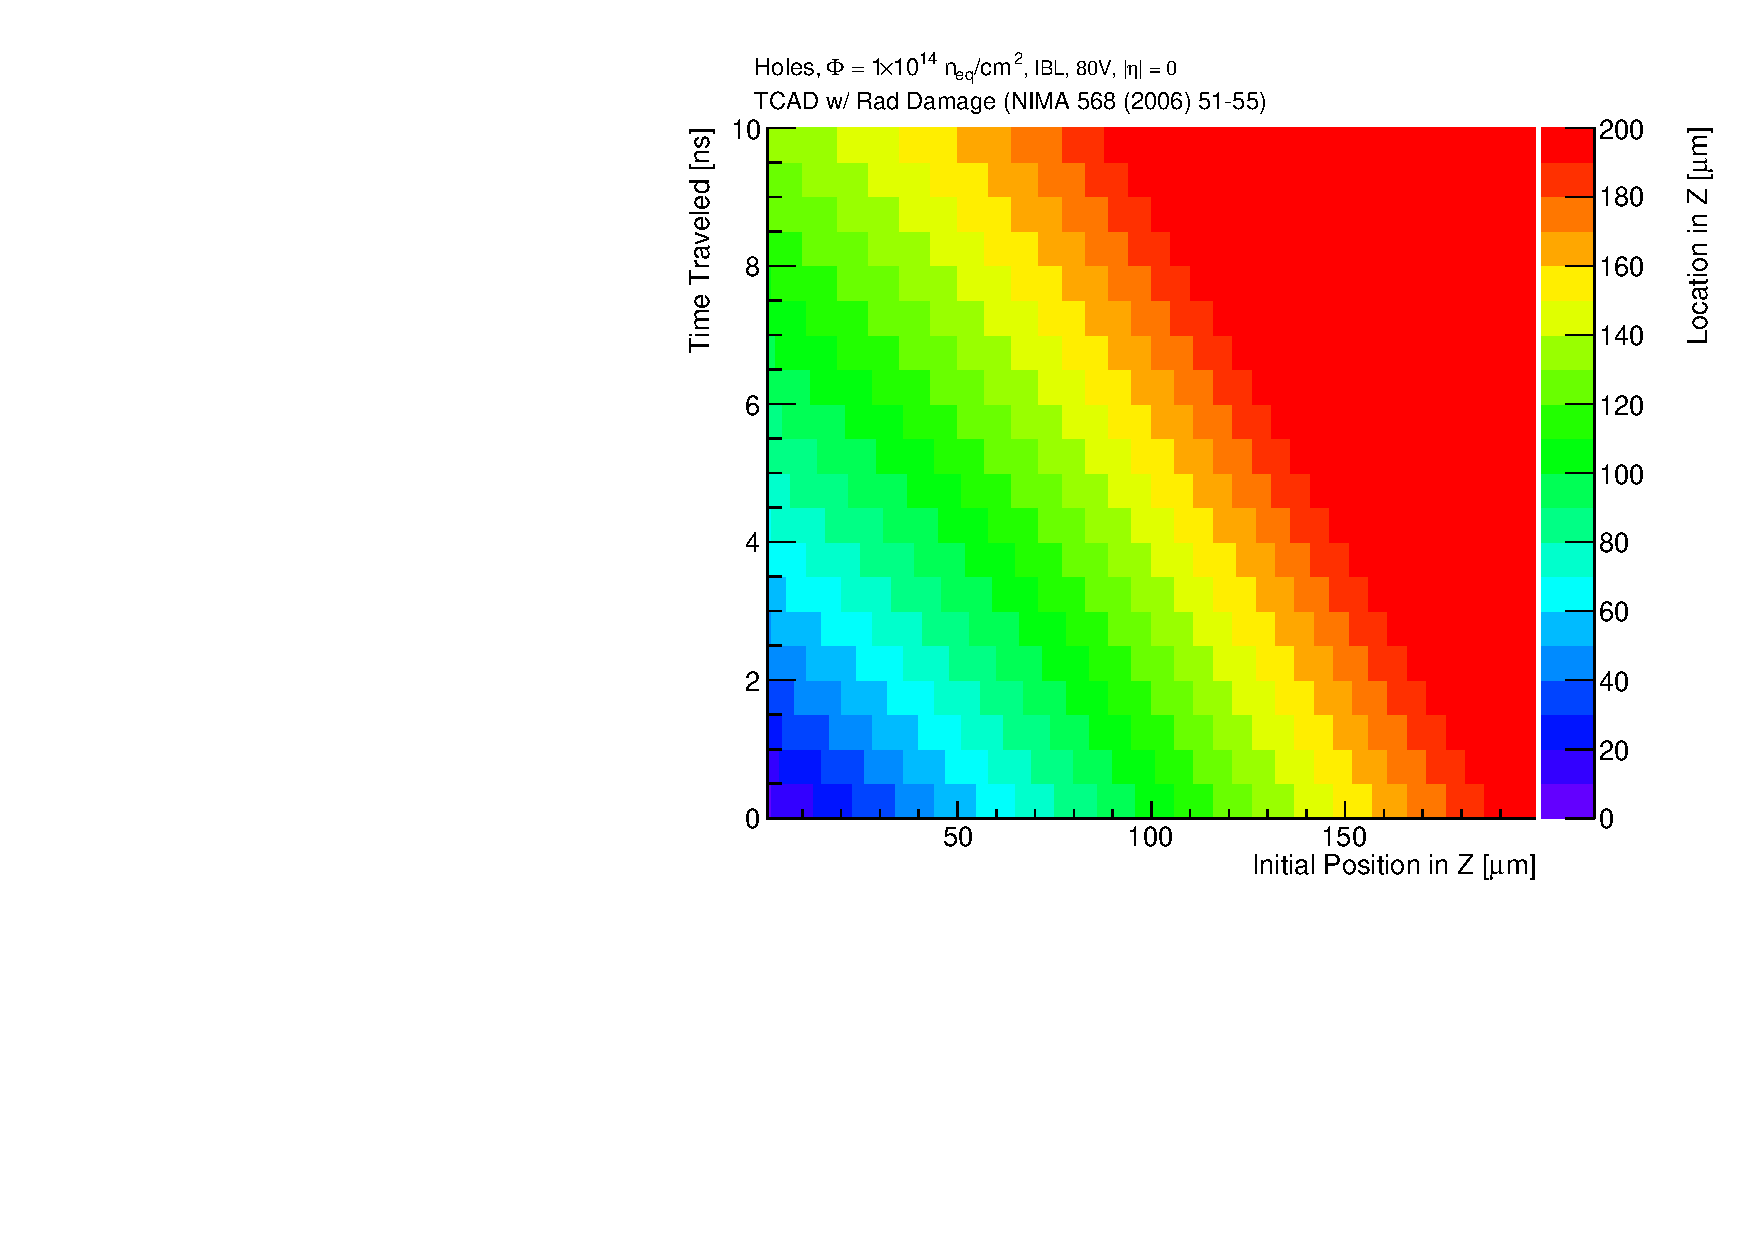
\includegraphics[width=0.49\textwidth]{distance_maps_h1e14.pdf}
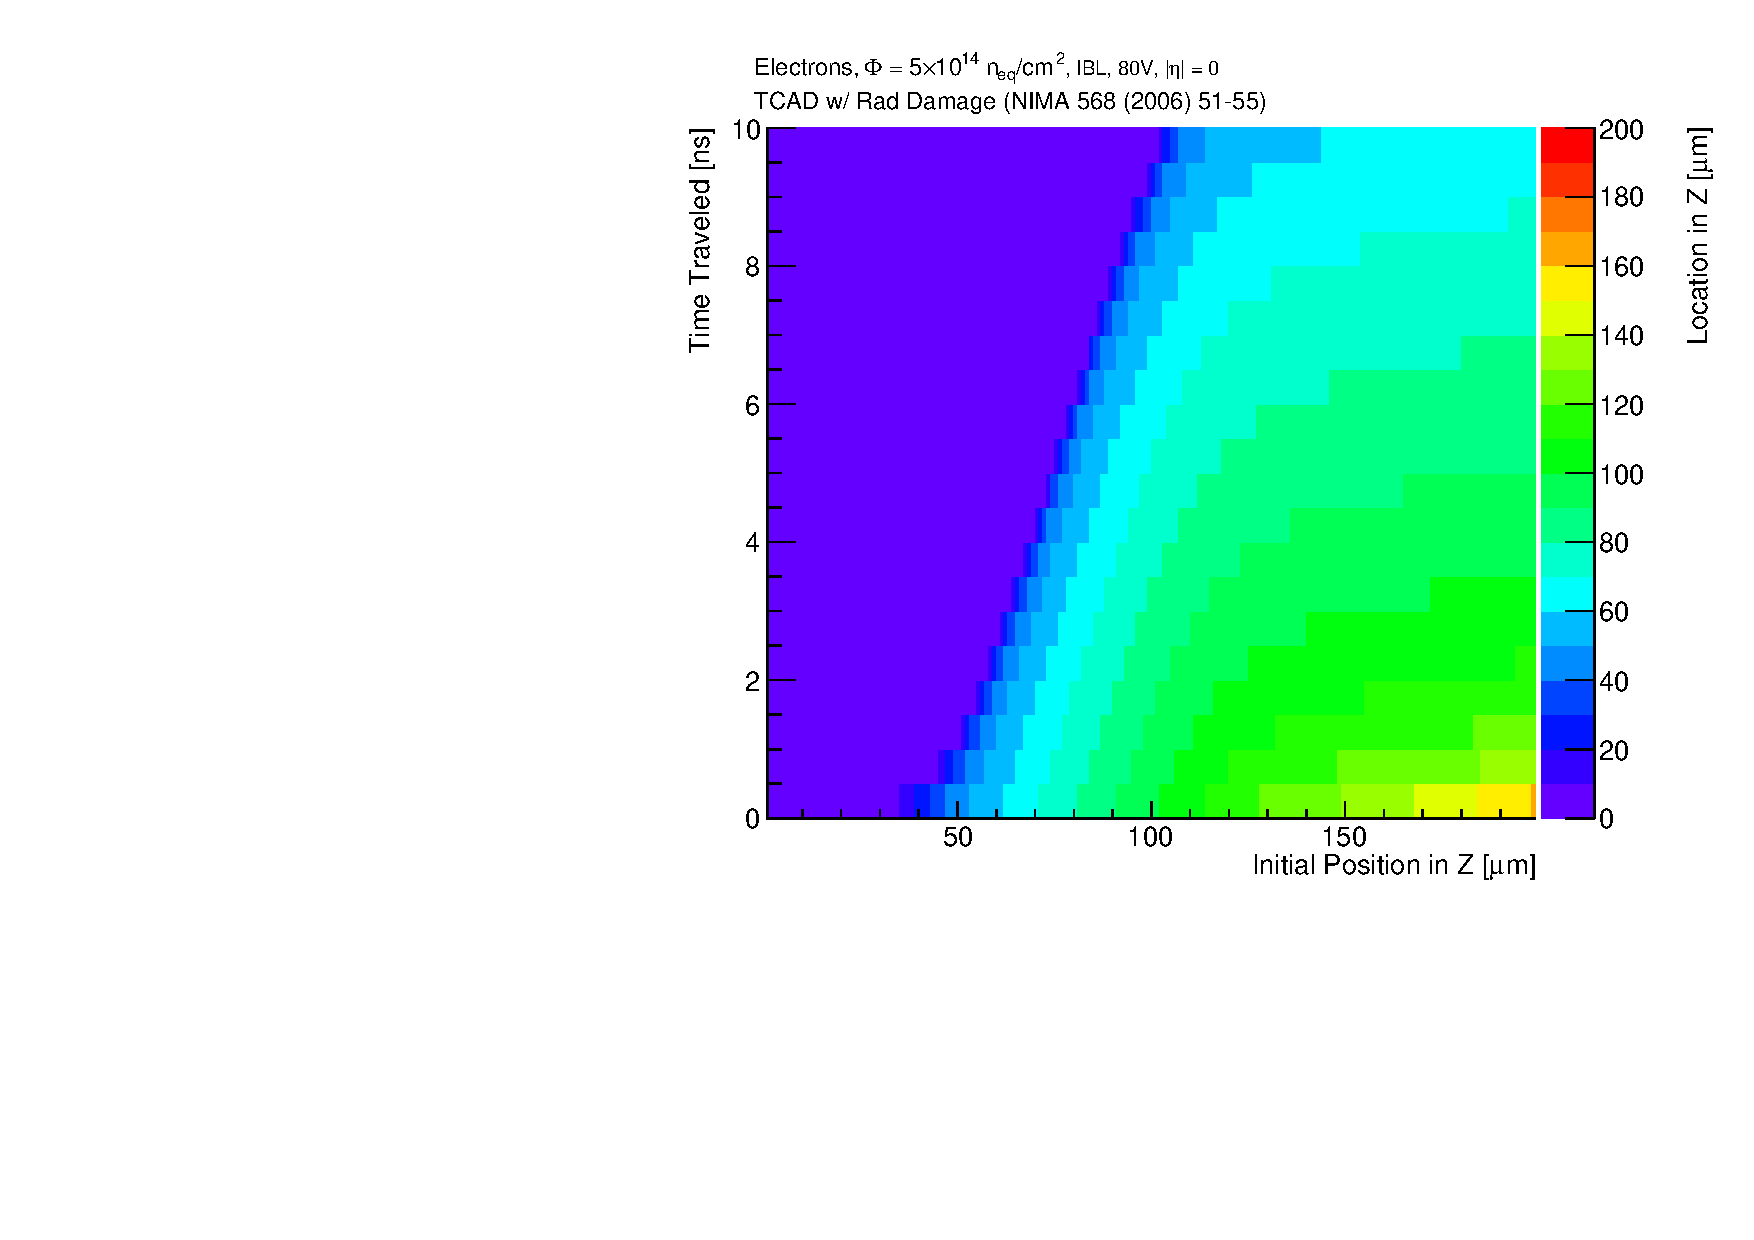
\includegraphics[width=0.49\textwidth]{distance_maps_e5e14.pdf}
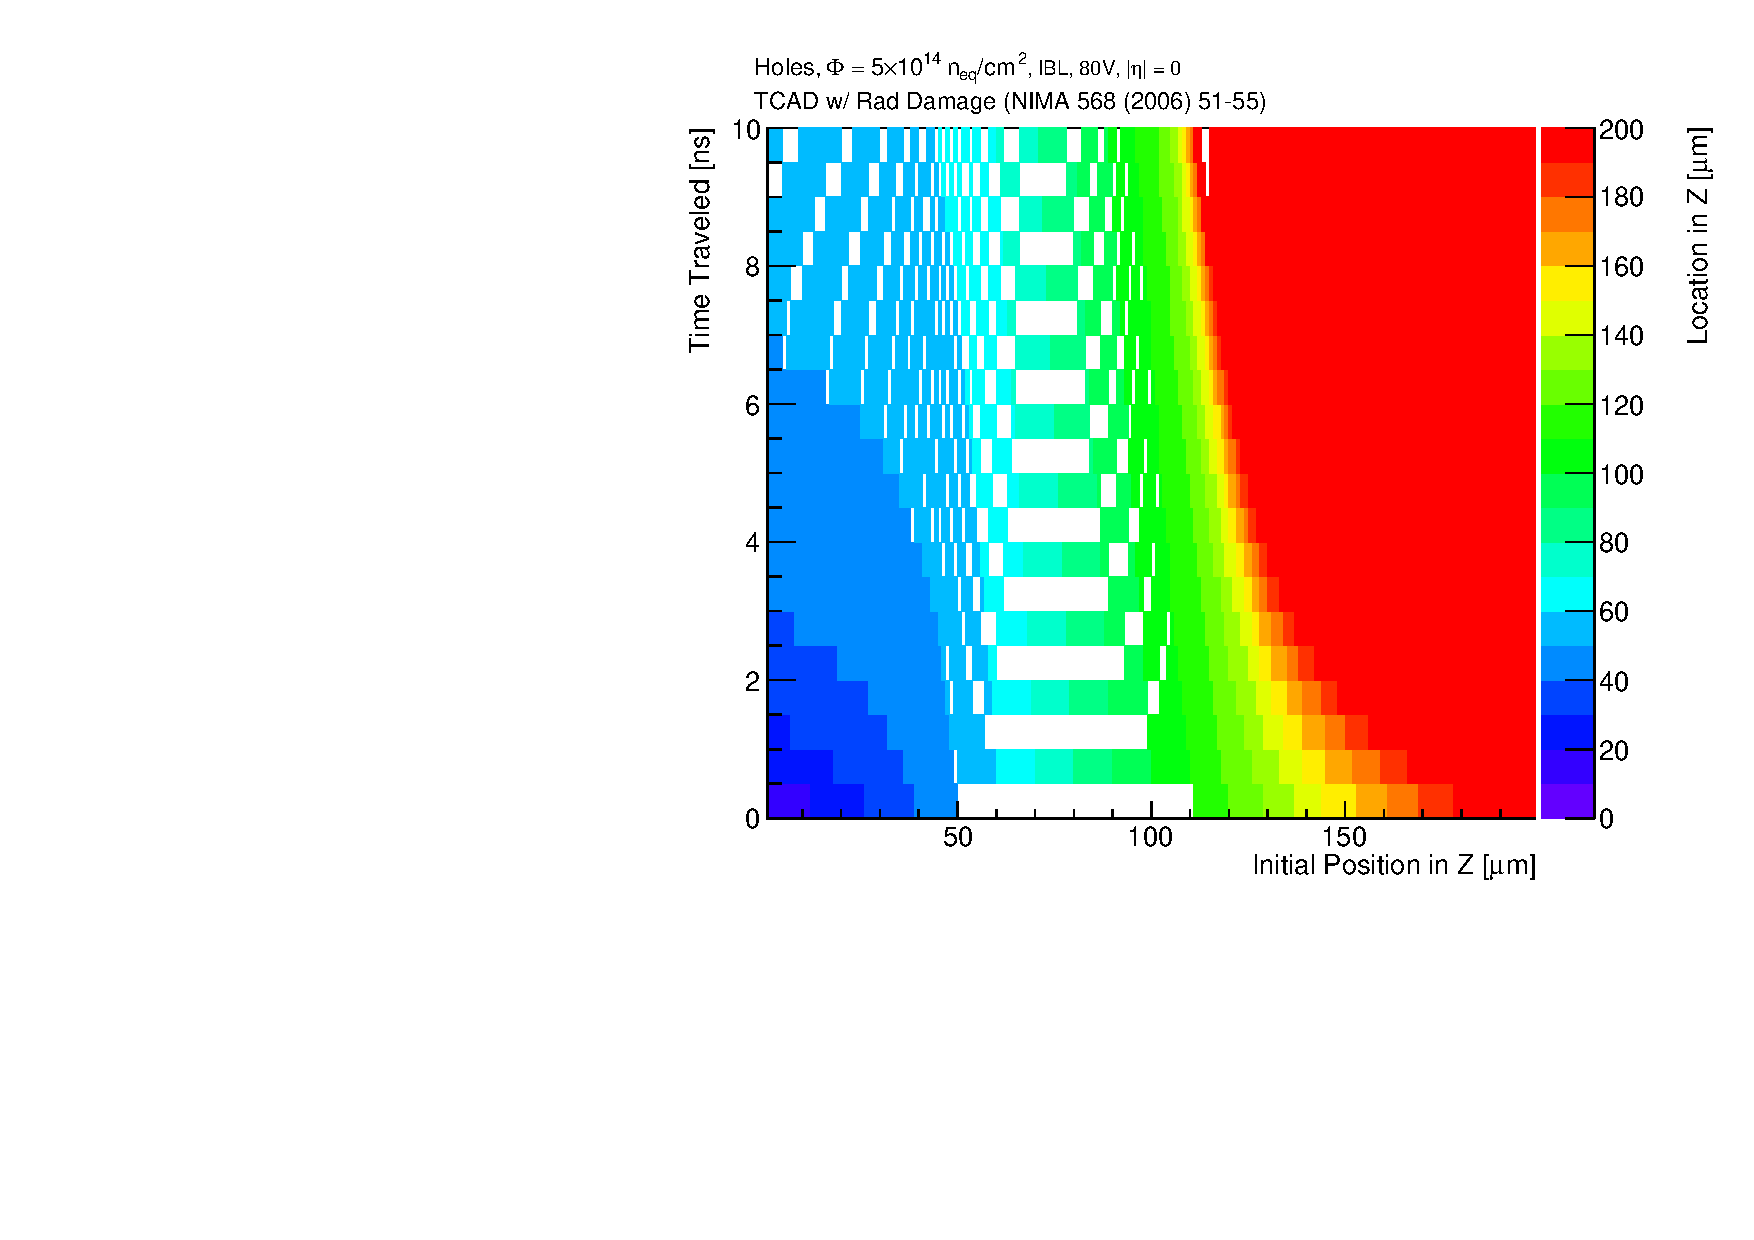
\includegraphics[width=0.49\textwidth]{distance_maps_h5e14.pdf}
\caption{The $z$ position of the trapped electrons (left) or holes (right) as a function of their starting position and the time traveled for $\Phi=10^{14}$ $n_\text{eq}/\text{cm}^2$ (left) and $\Phi=5\times10^{14}$ $n_\text{eq}/\text{cm}^2$ (right).  The collecting electrode is at origin while the backplane is at $200$ $\mu$m.  }
\label{fig:posattrap}
\end{figure}

\subsection{Lorentz angle}
\label{sec:mapsLorentz}

In addition to drifting with the electric field, electrons and holes also move in reaction to the 2 T magnetic field that surrounds the ATLAS inner detector.  Due to the orientation of the electrodes, this has nearly no impact on the 3D sensors, but is significant for planar sensors.  The tilt angle of charge carrier drift with respect to the pixel axis is called the \textit{Lorentz angle} and is given by $\tan\theta_L=r\mu(E) B$, where $r$ is the Hall scattering factor and $\mu(E)$ is the mobility as a function of the electric field, defined in Sec.~\ref{sec:maps}.  Due to the dependence of the electric field on the sensor depth, the Lorentz angle can change significantly along the trajectory of an electron or hole.  The left plot of figure~\ref{fig:lorentzangle:Run2} demonstrates the change in the Lorentz angle along the trajectory of electrons and holes.  As the mobility increases with decreasing electric field strength, the Lorentz angle is largest near the center of the sensors when irradiated.

The Lorentz angle can have important implications for charge sharing and it is therefore important to correct for the path dependence of the angle.  This is modeled in a similar manner to the maps from Sec~\ref{sec:Efieldmodelcomparisons} by integrating the Lorentz angle along the path:

\begin{align}
\label{eq:integratedlorentzangle}
\tan\theta_L^\text{integrated}(z_\text{initial},z_\text{final})=\frac{rB}{|z_\text{final}-z_\text{initial}|}\int_{z_\text{initial}}^{z_\text{final}}\mu(E(z)) dz.
\end{align}

The drift along the $\phi$ direction (the azimuthal angle transverse to the beam) is then modified as $|z_\text{final}-z_\text{initial}|\tan\theta_L^\text{integrated}(z_\text{initial},z_\text{final})$, where the direction is the same for both electrons and holes because both the charge and velocity sign are reversed for holes with respect to electrons. The size of the integrated Lorentz angle variations are shown in Fig.~\ref{fig:lorentzangle:Run2}; for this fluence and bias voltage, the integrated Lorentz angle can change by as much as a factor of two, depending on the starting and ending position.  

\begin{figure}[htpb!]
\centering
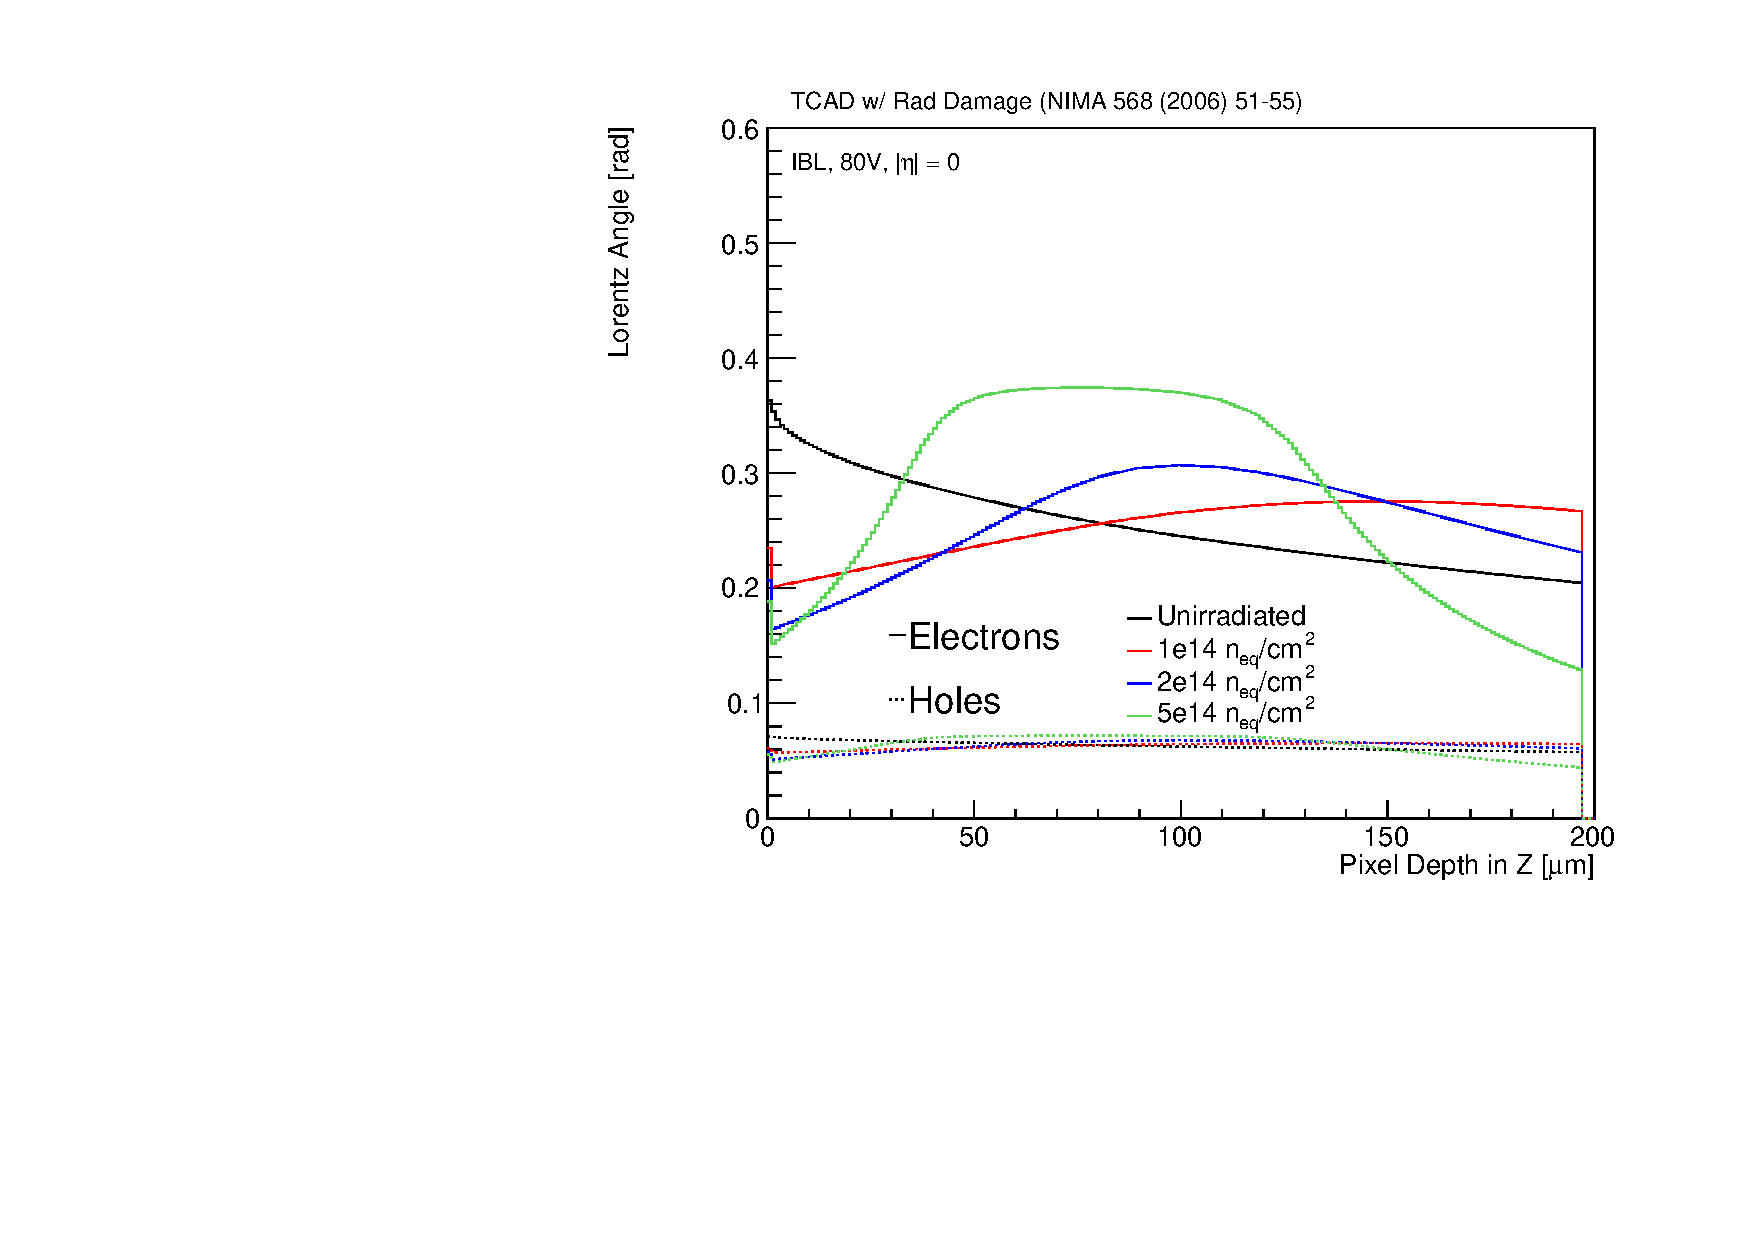
\includegraphics[width=0.49\textwidth]{Angle_0fluence80V.pdf}
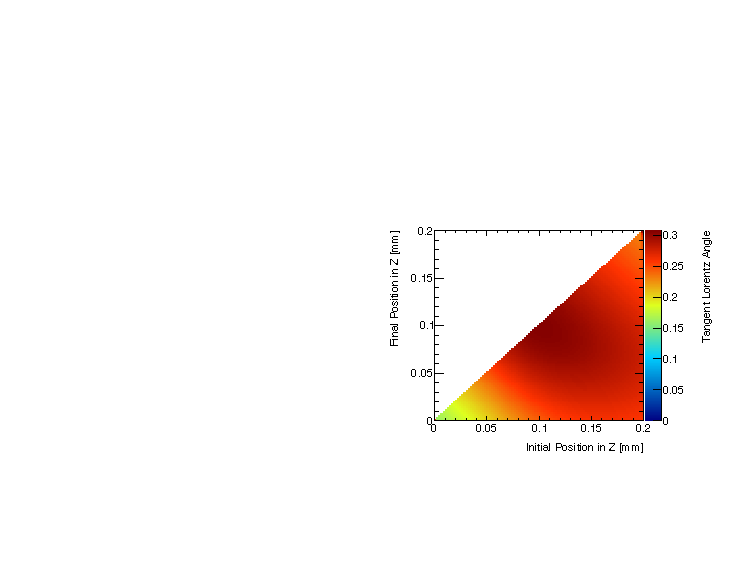
\includegraphics[width=0.49\textwidth]{Run2}
\caption{Left: The depth dependence of the Lorentz angle for electrons and holes for four fluences in an ATLAS IBL planar sensor biased at 80 V.  Right: The integrated Lorentz angle for electrons (see Eq.~\ref{eq:integratedlorentzangle}) as a function of the starting and ending position for a fluence of $\Phi=2\times10^{14}$ $n_\text{eq}/\text{cm}^2$.  The collecting electrode is at a $z$ position of $0$.}
\label{fig:lorentzangle:Run2}
\end{figure}


\subsection{Trapping}
\label{sec:chargetrapping}

As a result of irradiation, defects form in the silicon and are sites for charge trapping.  In the simulation, charge chunks are declared trapped if the projected time to reach the electrode from Sec.~\ref{sec:maps} exceeds a random trapping time $t$ that is exponentially distributed with mean value $1/(\kappa\Theta)$, where $\Theta$ is the fluence.  The constant $\kappa$ (sometimes called $\beta$ in the literature) has been measured at the 2001 CERN test beam and is approximately $\kappa=3\times 10^{-16}$ cm${}^2$/ns~\cite{trapping2}.  Charge trapping reduces the collected signal and thus degrades track reconstruction efficiency.

\subsection{Ramo Potential and the Induced Charge}
\label{sec:ramo}

Even though radiation damage causes charges to be trapped, the measured signal need not be zero.  This is because charge is registered as soon as the electrons or holes start to move.  One can compute the total induced charge without modeling the detailed time-dependent current via the the \textit{Ramo potential} from the Shockley-Ramo theorem~\cite{Shockley,Ramo}.  This theorem states that the amount of induced charge is the particle charge multiplied by the difference in the Ramo potential $\phi$ from its starting and ending (trapped) location:

\begin{align}
\label{eq:ramo}
Q_\text{induced} = -Q[\phi(\vec{x}_\text{end})-\phi(\vec{x}_\text{start})],
\end{align}

where $Q$ is the charge of the drifting carrier.  The Ramo potential for a particular electrode is computed by calculating the electrostatic potential with the boundary condition of the electrode held at unit voltage and setting all other electrodes to have zero potential.  For example, for a an infinite parallel plate capacitor, the field is constant in between the plates, so the Ramo potential is linear (starting at 1 and decreasing to zero).  This potential depends only on geometry and therefore can be computed once prior to any event simulation.   Figure~\ref{fig:ramo:schematic} schematically demonstrates the combination of charge trapping and the Ramo potential by re-simulating three initial electrons many times, including diffusion.  As the electrons drift toward the electrode under the influence of the electric field, there is a chance that they are trapped.  If the electrons do not move very far, the induced charge is small compared to the charged induced if they travel nearly the entire distance to the electrode.  Note that the charge of one electron is only induced if both the electron and hole in one pair travel their full drift distance.  Since the Ramo potential of the collecting electrode is 1 and that of the backplane or $p^+$ electrode is zero: $Q_\text{induced}^e+Q_\text{induced}^h=-Q[\phi(\vec{x}_\text{end}^e)-\phi(\vec{x}_\text{end}^h)]=-Q[1-0]=-Q$.  This is what is meant by charge being `collected'.

\begin{figure}[!htpb]
\centering
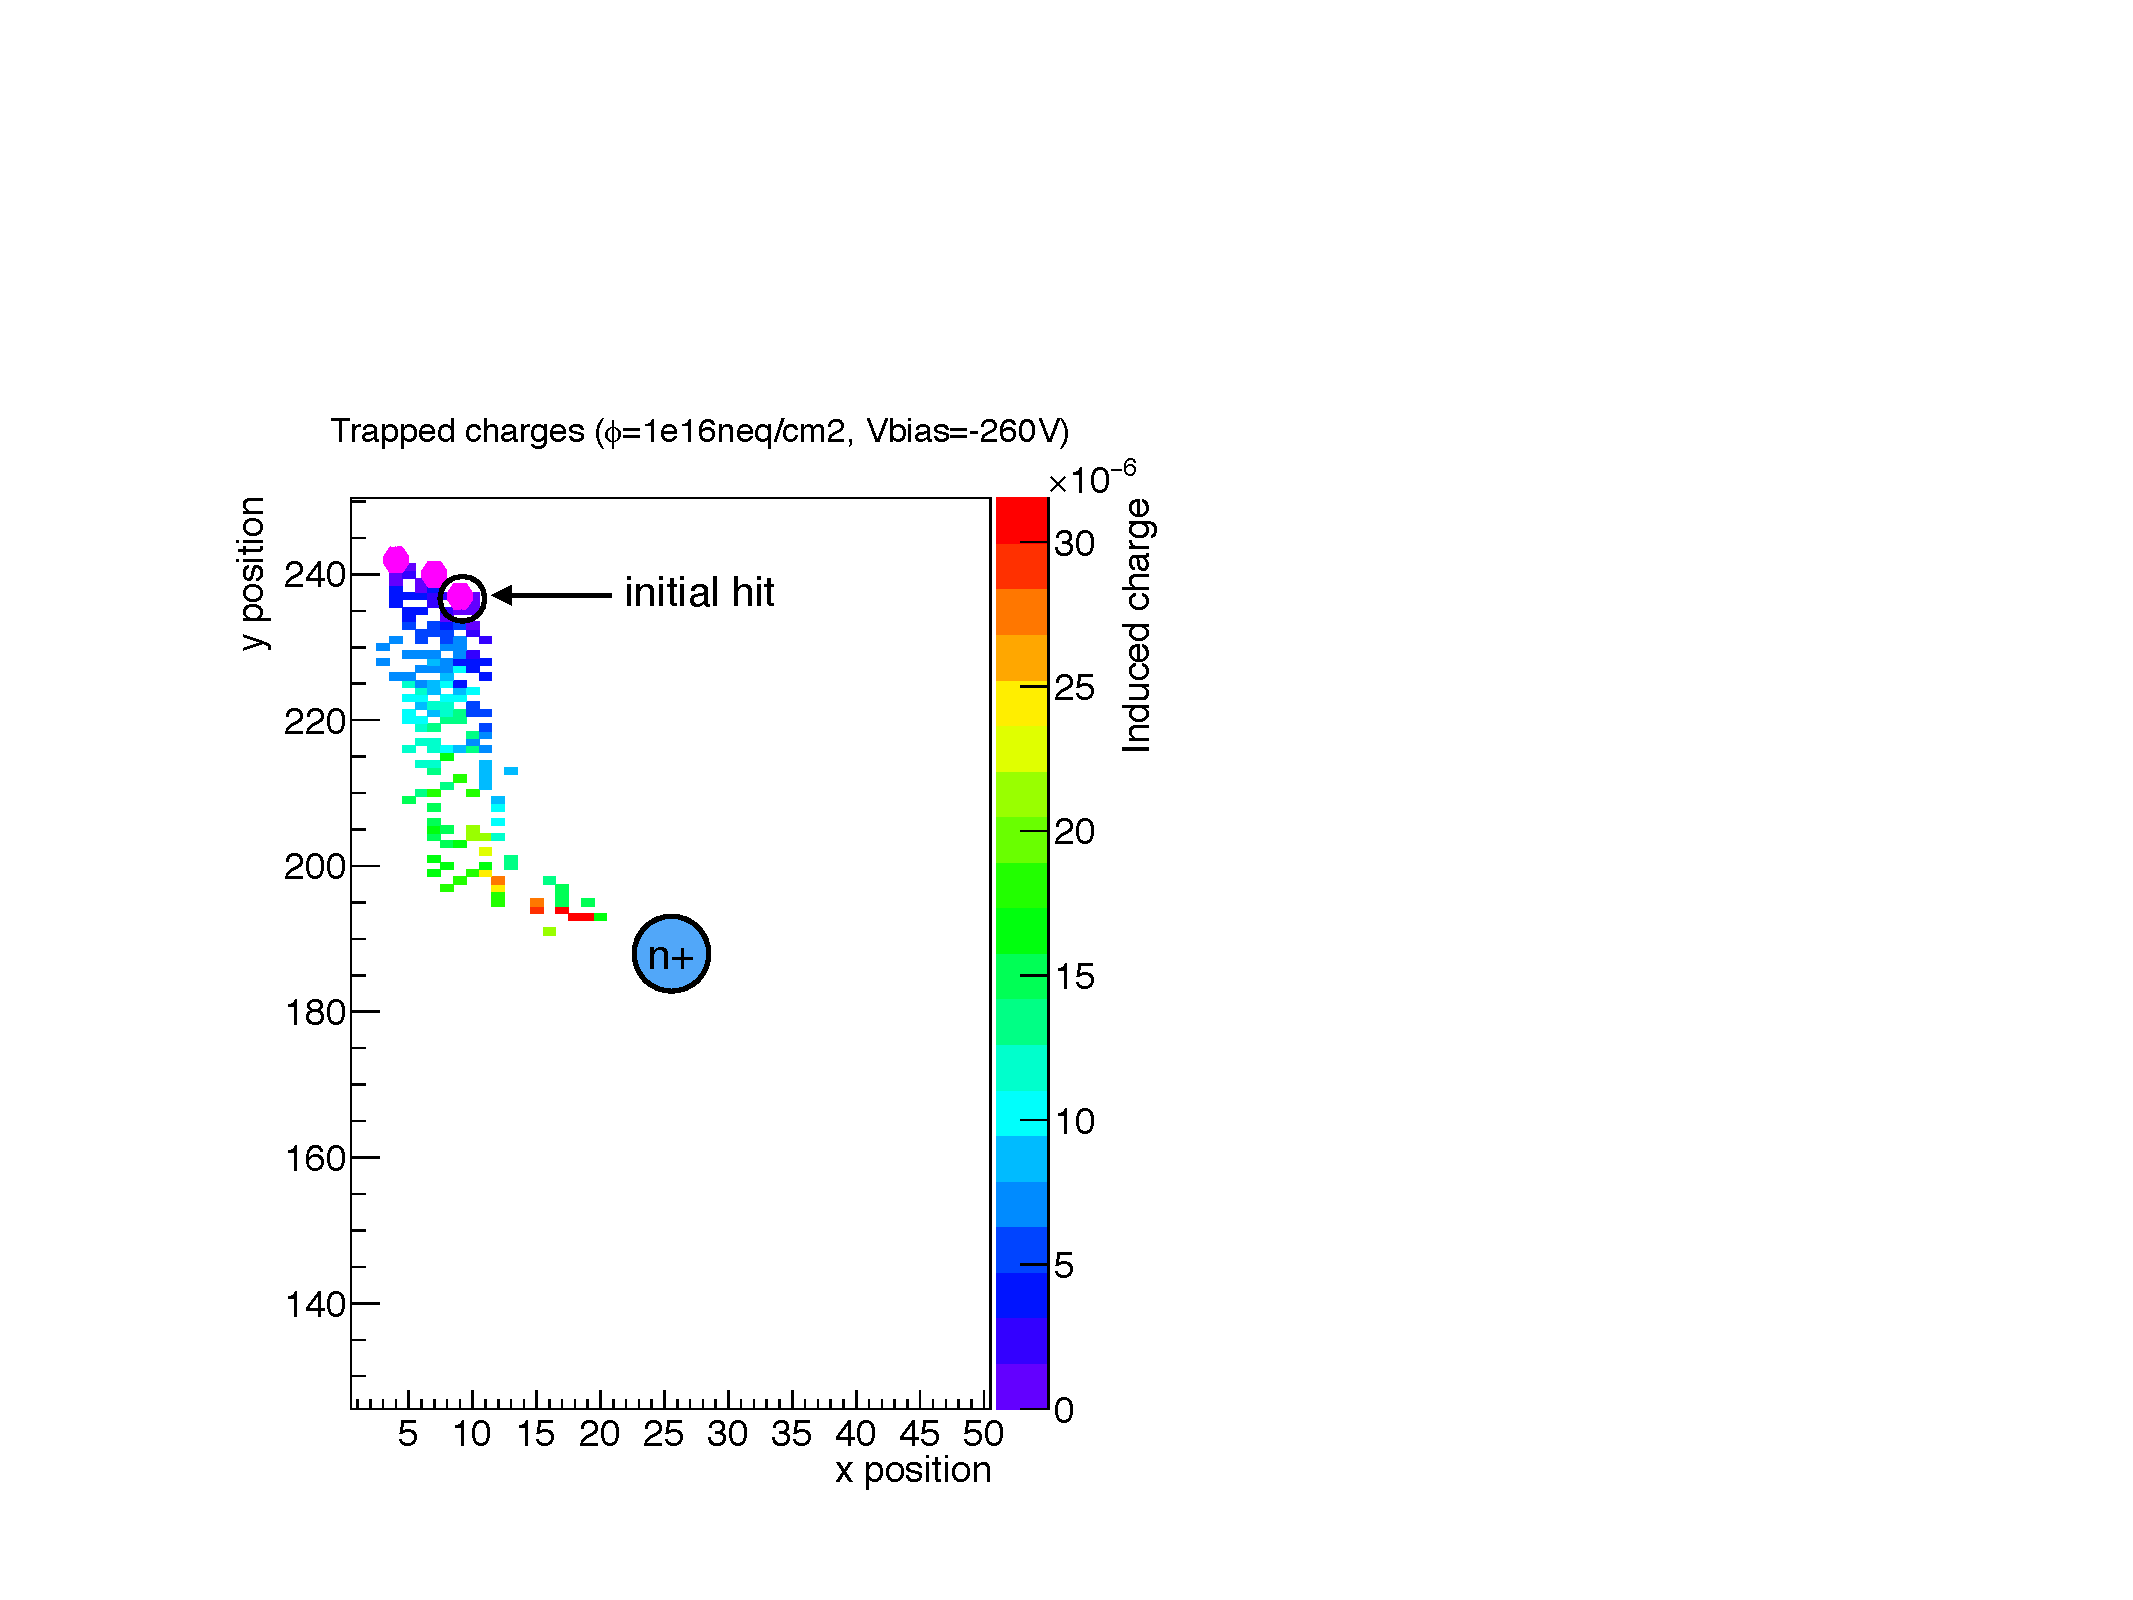
\includegraphics[width=0.33\textwidth]{ramoschematic3D.pdf}
\caption{An illustration of charge trapping and the Ramo potential in one-half of a 3D sensor.  Three initial electrons are ionized in the top left corner of the plot.  Under the influence of the electric field, they drift toward the $n^+$ electrode in the center.  As they drift, there is a chance that they get trapped.  Markers indicate the location of trapped charges and the color shows the charged induced on the $n^+$ electrode.  The process is repeated many times, with diffusion.}
\label{fig:ramo:schematic}
\end{figure}

The Ramo potential is calculated using TCAD to solve the Poisson's equation.  For planar sensors, most of the variation in the Ramo potential is in the $z$ direction, but one must include the $x$ and $y$ dependence in order to account for charge induced on the neighboring pixels.  The left plot of Fig.~\ref{fig:ramo:planar} shows a slice of the three-dimensional Ramo potential at $x=0$.  Vertical lines indicate the position of the pixels: the potential can be as much as $20$-$30\%$ in the nearest neighboring pixel.  The right plot of Fig.~\ref{fig:ramo:planar} shows a one-dimensional projection of the Ramo potential along the $z$ axis.  Due to the simple geometry of a planar sensor, the full TCAD simulation is well-approximated by a series expansion that solves Poisson's equation with periodic boundary conditions.  The expansion matches the full three-dimensional potential well and is shown in the right plot of Fig.~\ref{fig:ramo:planar} for illustration.  In the digitizer code, if the user does not supply a Ramo potential calculated with TCAD, this series expansion is substituted instead so that geometries for which a TCAD model has not yet been created can be studied.  The $z$-dependence of the planar Ramo potential alone is also very well approximated by a double exponential of the form 

\begin{align}
\label{eq:doublexp}
\phi_z(z)=[e^{-z/\alpha L}+e^{-z/L}-e^{-\alpha}-e^{-1}]/(2-e^{-\alpha}-e^{-1}),
\end{align}

where $L=200$ $\mu m$ and the denominator is chosen to make $\phi_z(0)=1$.  Good agreement is found for $\alpha\sim 3L/p$, where $p$ is the sensor pitch in the short direction (see Fig.~\ref{fig:ramo:planar}). 
\begin{figure}[!htpb]
\centering
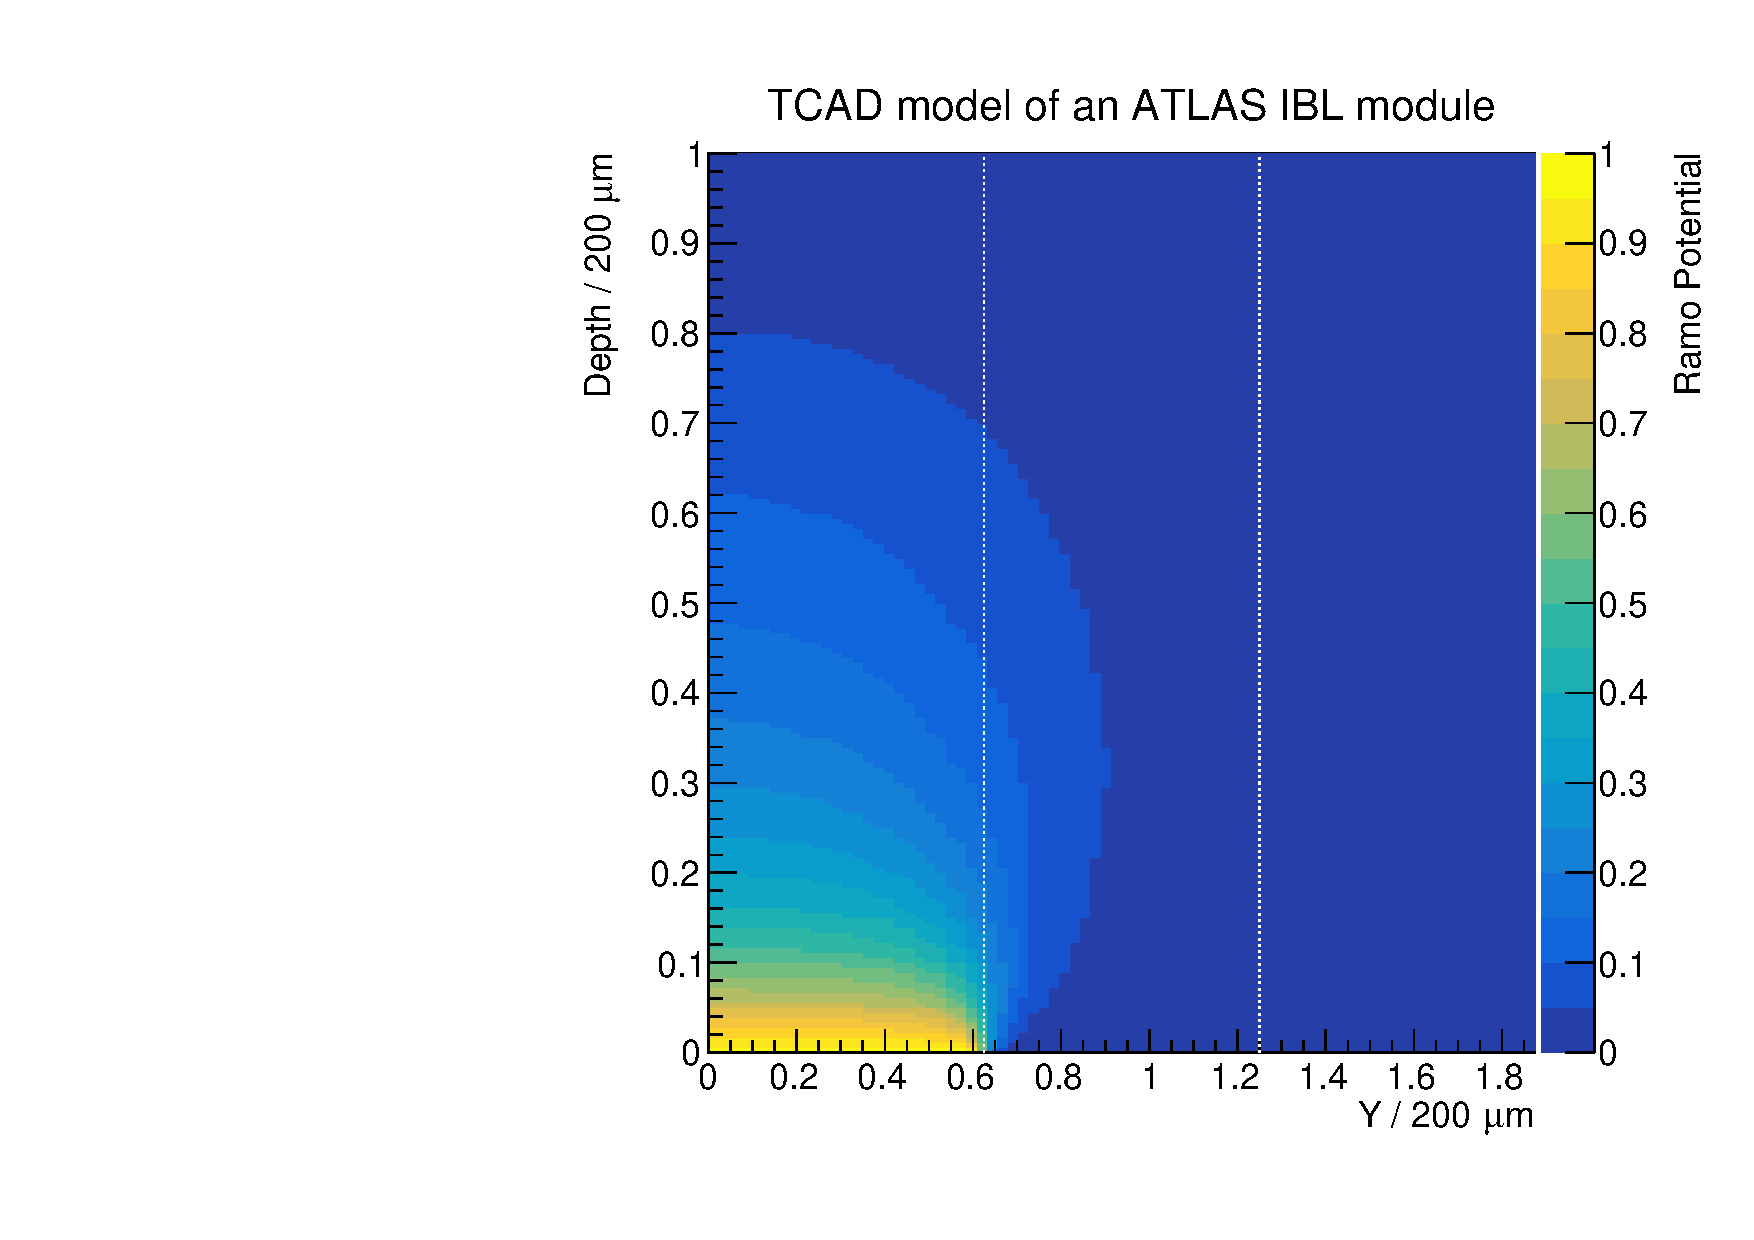
\includegraphics[width=0.49\textwidth]{test_ramoxz_10.pdf}
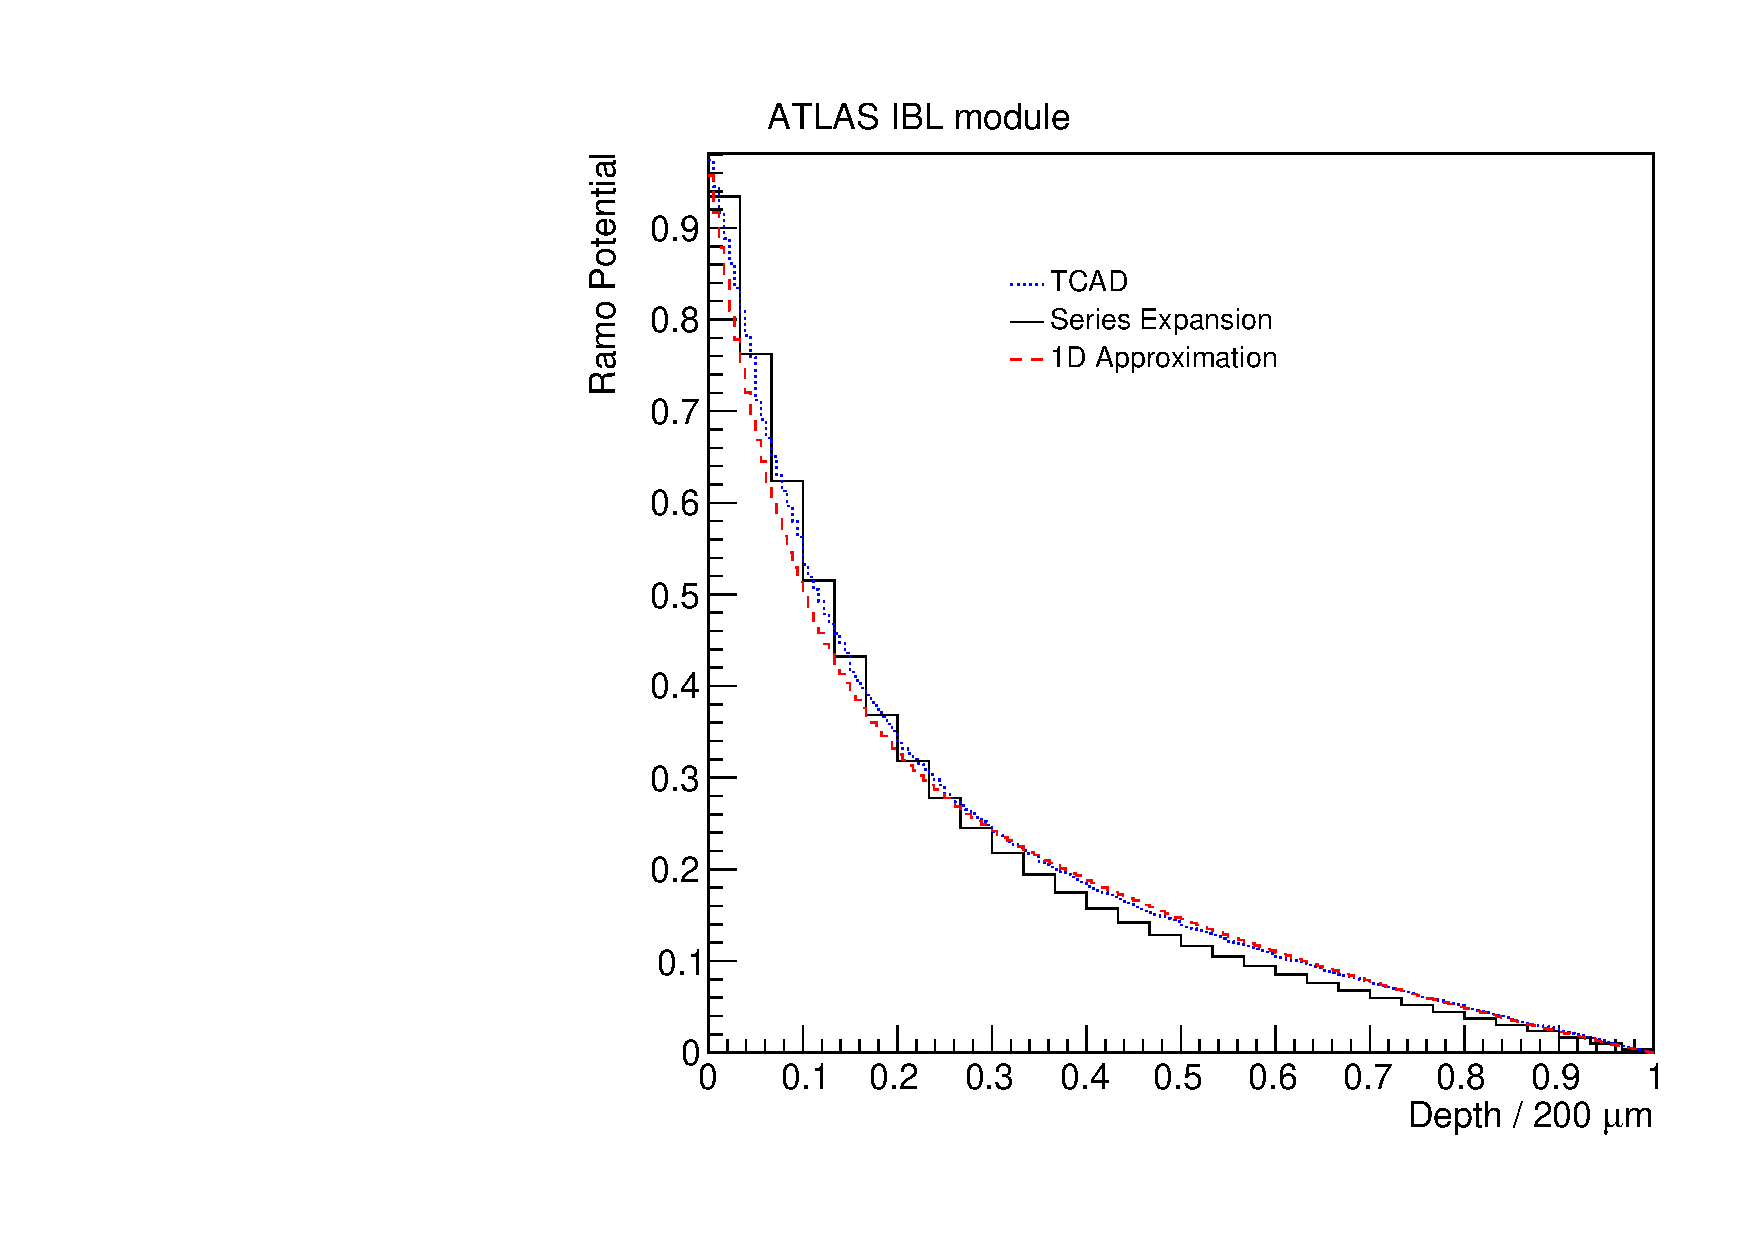
\includegraphics[width=0.49\textwidth]{test_ramoz_10.pdf}
\caption{Left: A two-dimensional slice of the full three-dimensional ATLAS planar sensor Ramo potential as computed with TCAD at $x=0$.  Dashed vertical lines indicate pixel boundaries.  Right: A one-dimensional slice of the Ramo potential at $x=y=0$.  Overlaid on top of the TCAD simulation are a series expansion solution of the Poisson's equation as well as double-exponential defined by Eq.~\ref{eq:doublexp}.}
\label{fig:ramo:planar}
\end{figure}

The implementation of the Ramo potential and charge trapping are illustrated in Fig.~\ref{fig:ramo:check} for planar sensors.  On the electrode from the same pixel as the electrons and holes originate, the induced charge equals the electron charge as the time to be trapped exceeds the time to drift toward the electrode.   The average collected charge is an asymmetric function of the depth inside the sensor because the drift and trapping times are different for electrons and holes and the Ramo potential is very asymmetric: the average fraction is lower far away from the collecting electrode.  In addition to inducing a charge on the electrode from the same pixel as the electron-hole pair generation, charge is induced in the neighboring pixels.  This is demonstrated in the middle and right plots of Fig.~\ref{fig:ramo:check}.  In the limit where the induced charge is the electron charge in the same pixel as the electron-hole pair, the induced charge in the neighbors approaches zero.  For some combinations of starting location and time to trap, the induced charge can even be negative.  This happens when holes are trapped very close to the pixel implants.  Even though the Ramo potential map extends beyond one neighbor pixel, in practice the nearest neighbor pixels are considered in the simulation.  The right plot of Fig.~\ref{fig:ramo:check} indicates that this is good approximation.

\begin{figure}[!htpb]
\centering
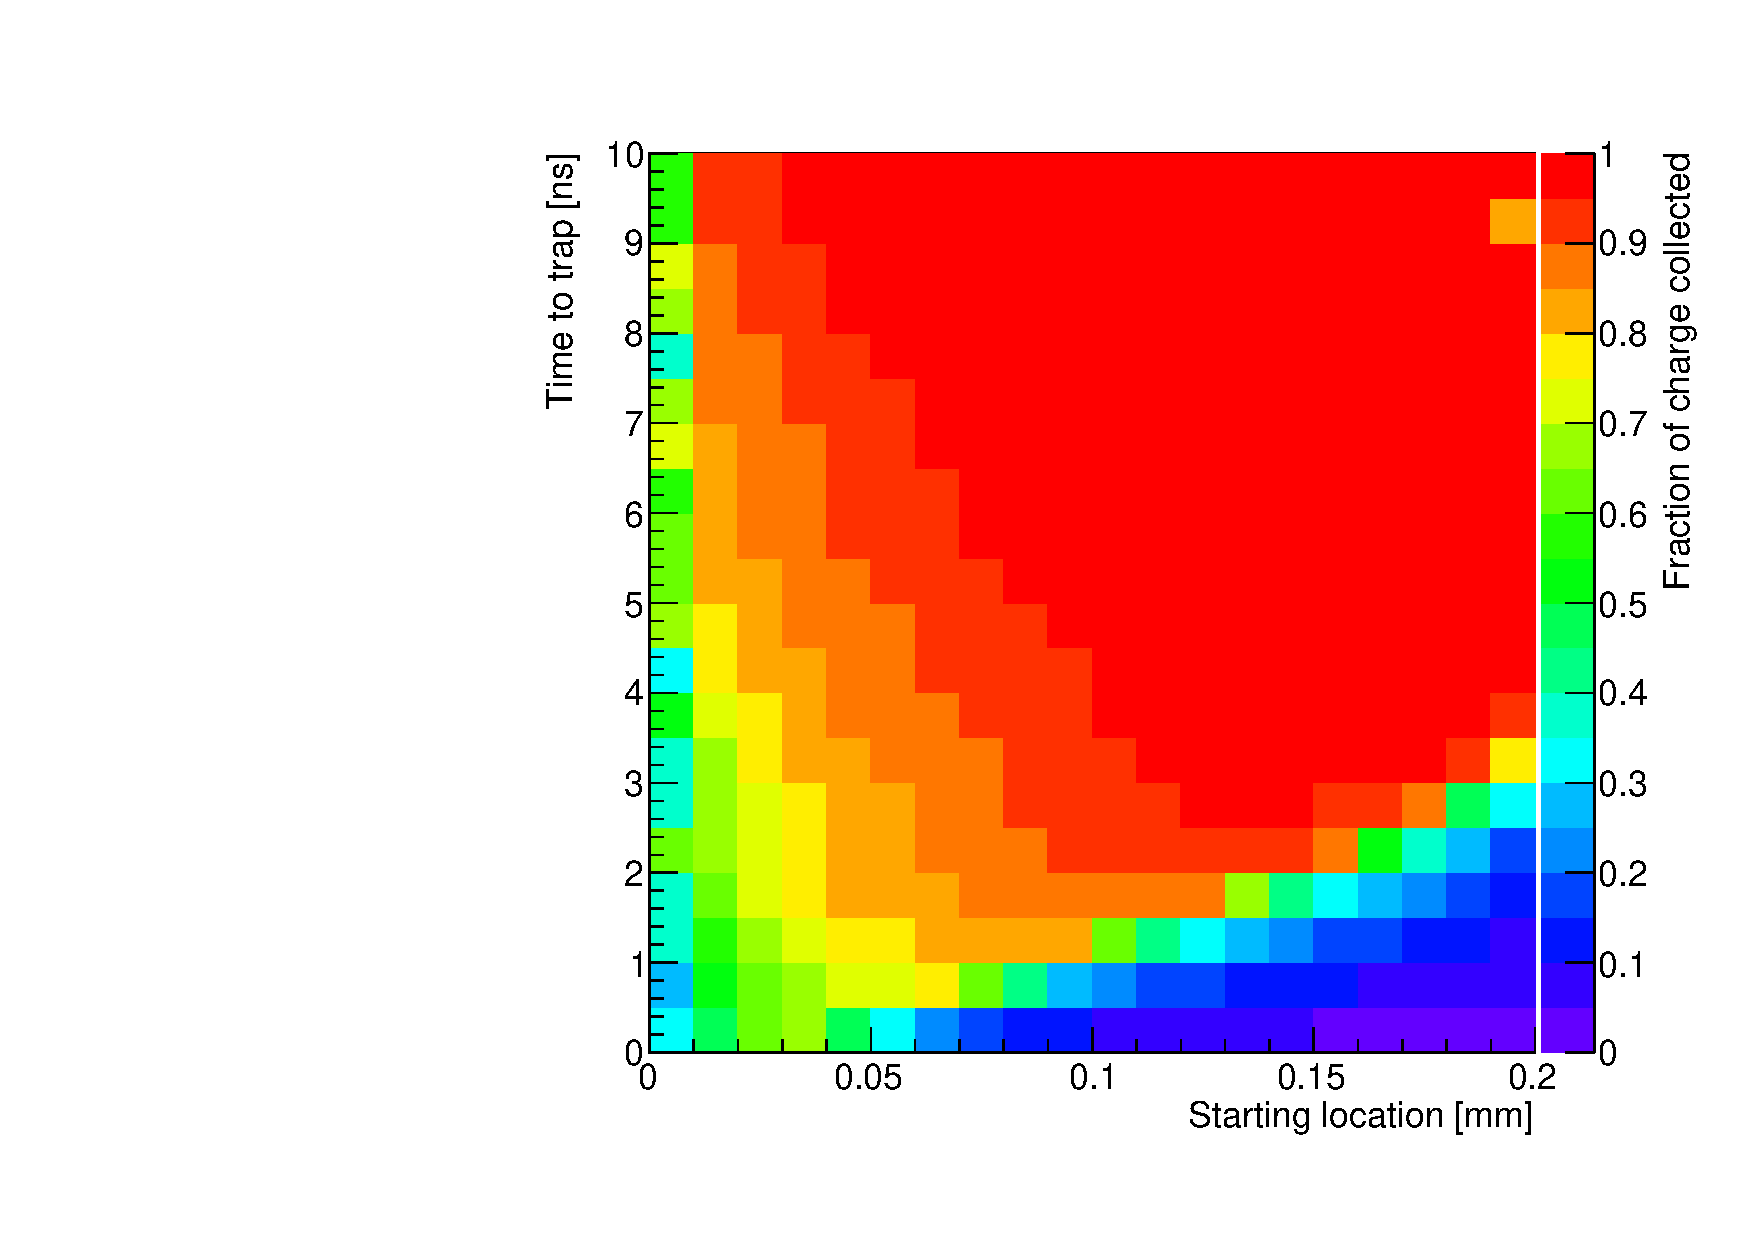
\includegraphics[width=0.32\textwidth]{testramo_corrected_other.pdf}
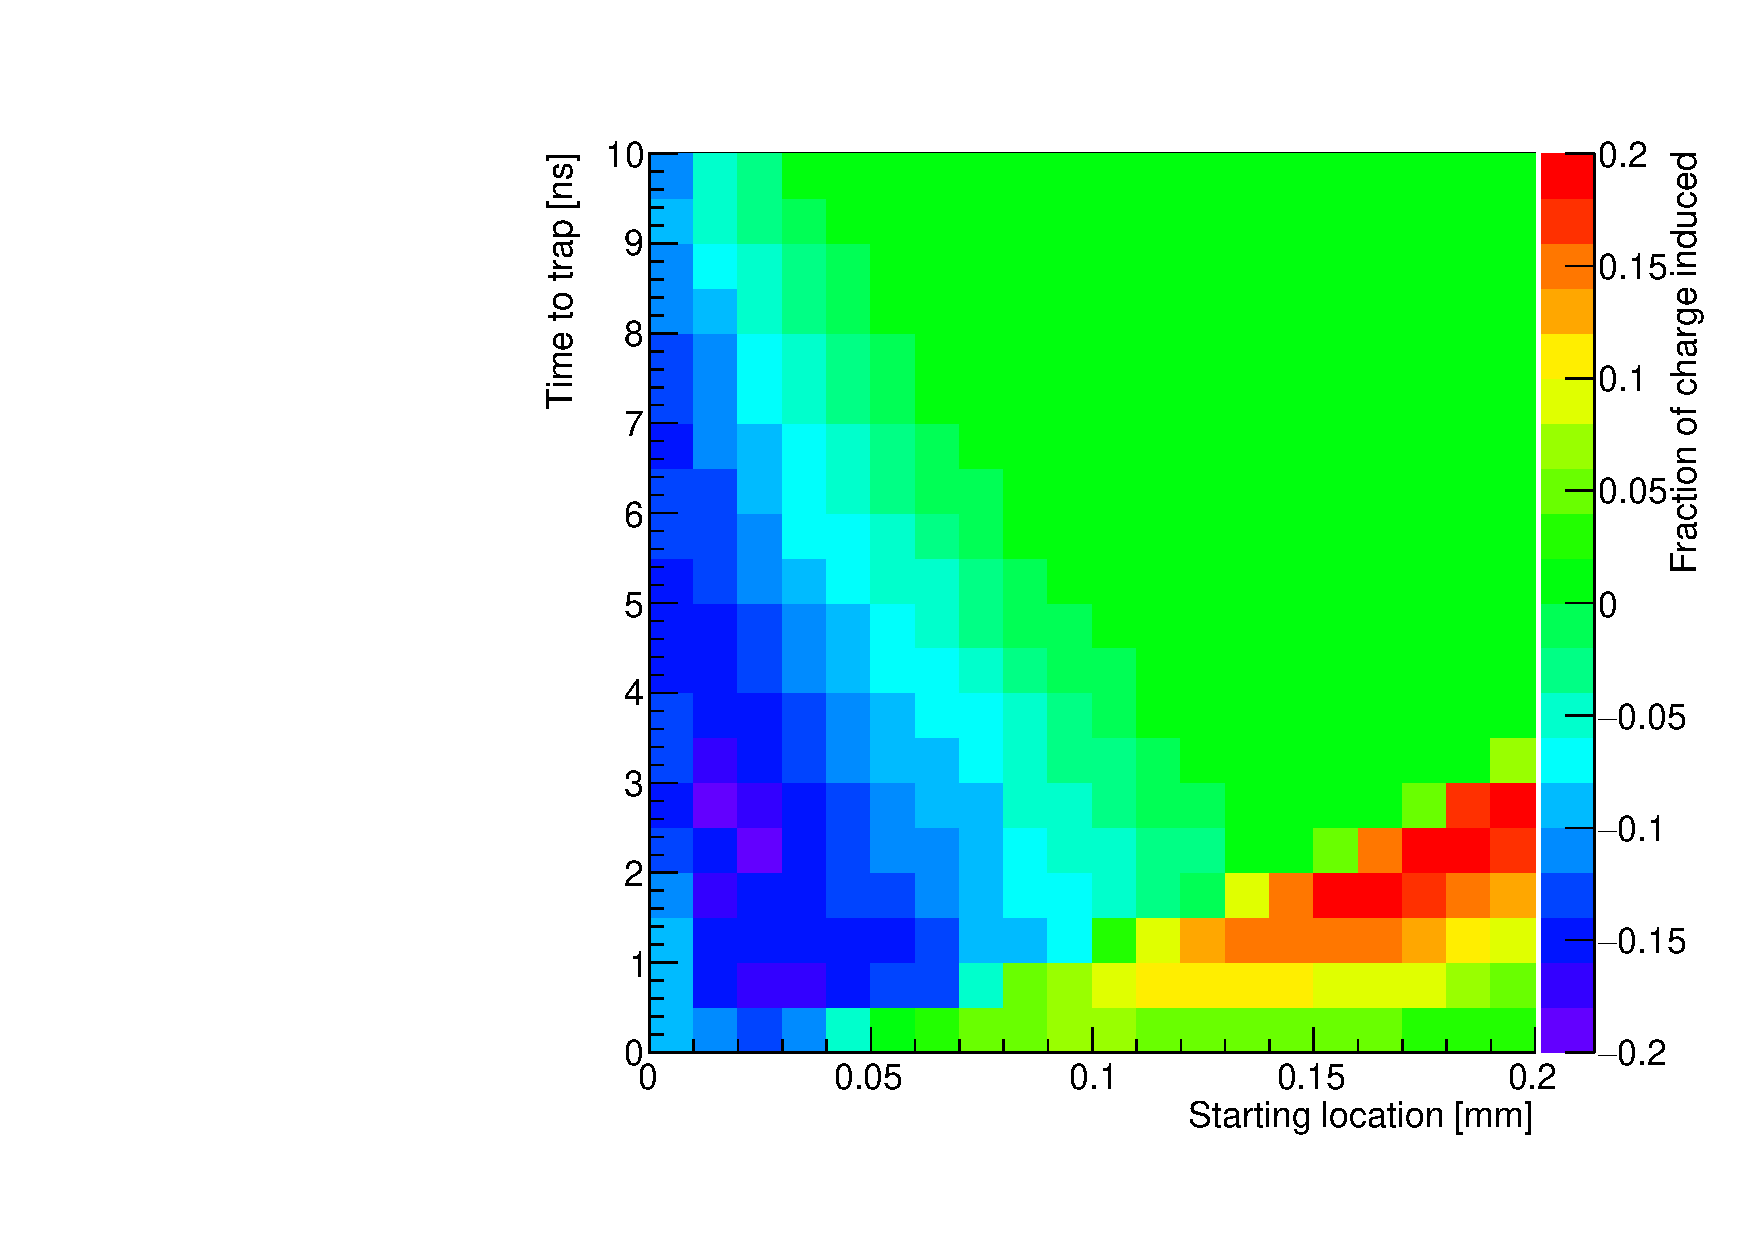
\includegraphics[width=0.32\textwidth]{testramo_induced_0_1.pdf}
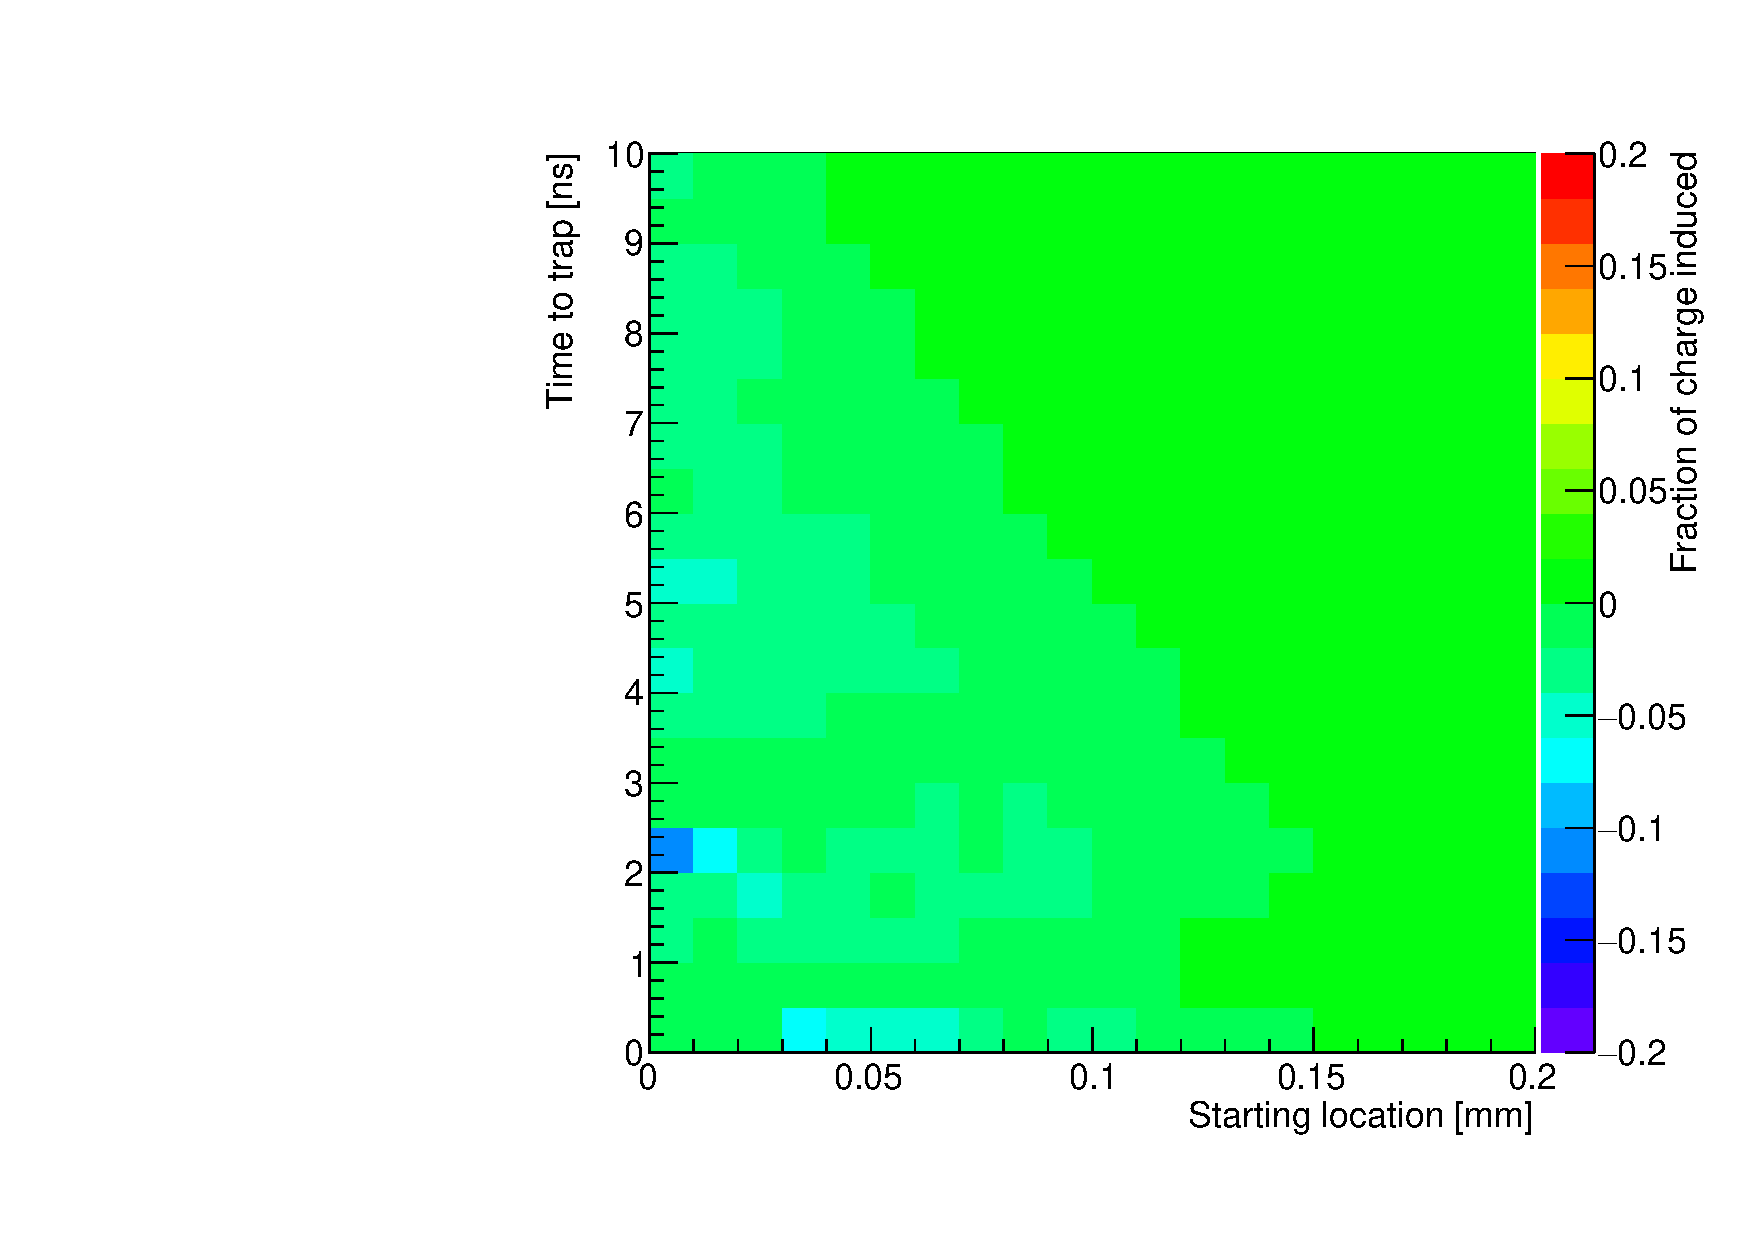
\includegraphics[width=0.32\textwidth]{testramo_induced_1_0.pdf}
\caption{The average charge collected as a function of the starting location and the time to be trapped for the same pixel as the electron-hole pair generation (left), the neighbor pixel in the short ($50$ $\mu $m) pitch direction (middle) and the pixel in the long pitch direction ($250$ $\mu m$) (right).  For simplicity, the electric field field is simulated without radiation damage and the vertical axis is a hypothetical trapping time.}
\label{fig:ramo:check}
\end{figure}

The Ramo potential for 3D sensors is slightly more involved than for planar sensors because the $n^+$ electrode have a non-trivial structure.  In particular, the two $n^+$ columns in one pixel are electrically connected and so in the calculation of the Ramo potential, both are held at unit potential while all other electrodes are grounded.  Therefore, the calculation requires a relatively large simulation area.  This is illustrated in Fig.~\ref{fig:ramo:3D}.  Unlike the Ramo potential for planar sensors, there is no relevant $z$ dependence of the potential so the entire function can be represented as a two-dimensional heat map.  As with the planar sensors, only the immediate neighbors are included in the calculation.  The numbers overlaid on Fig.~\ref{fig:ramo:3D} show that this is a good approximation. 

\begin{figure}[!htpb]
\centering
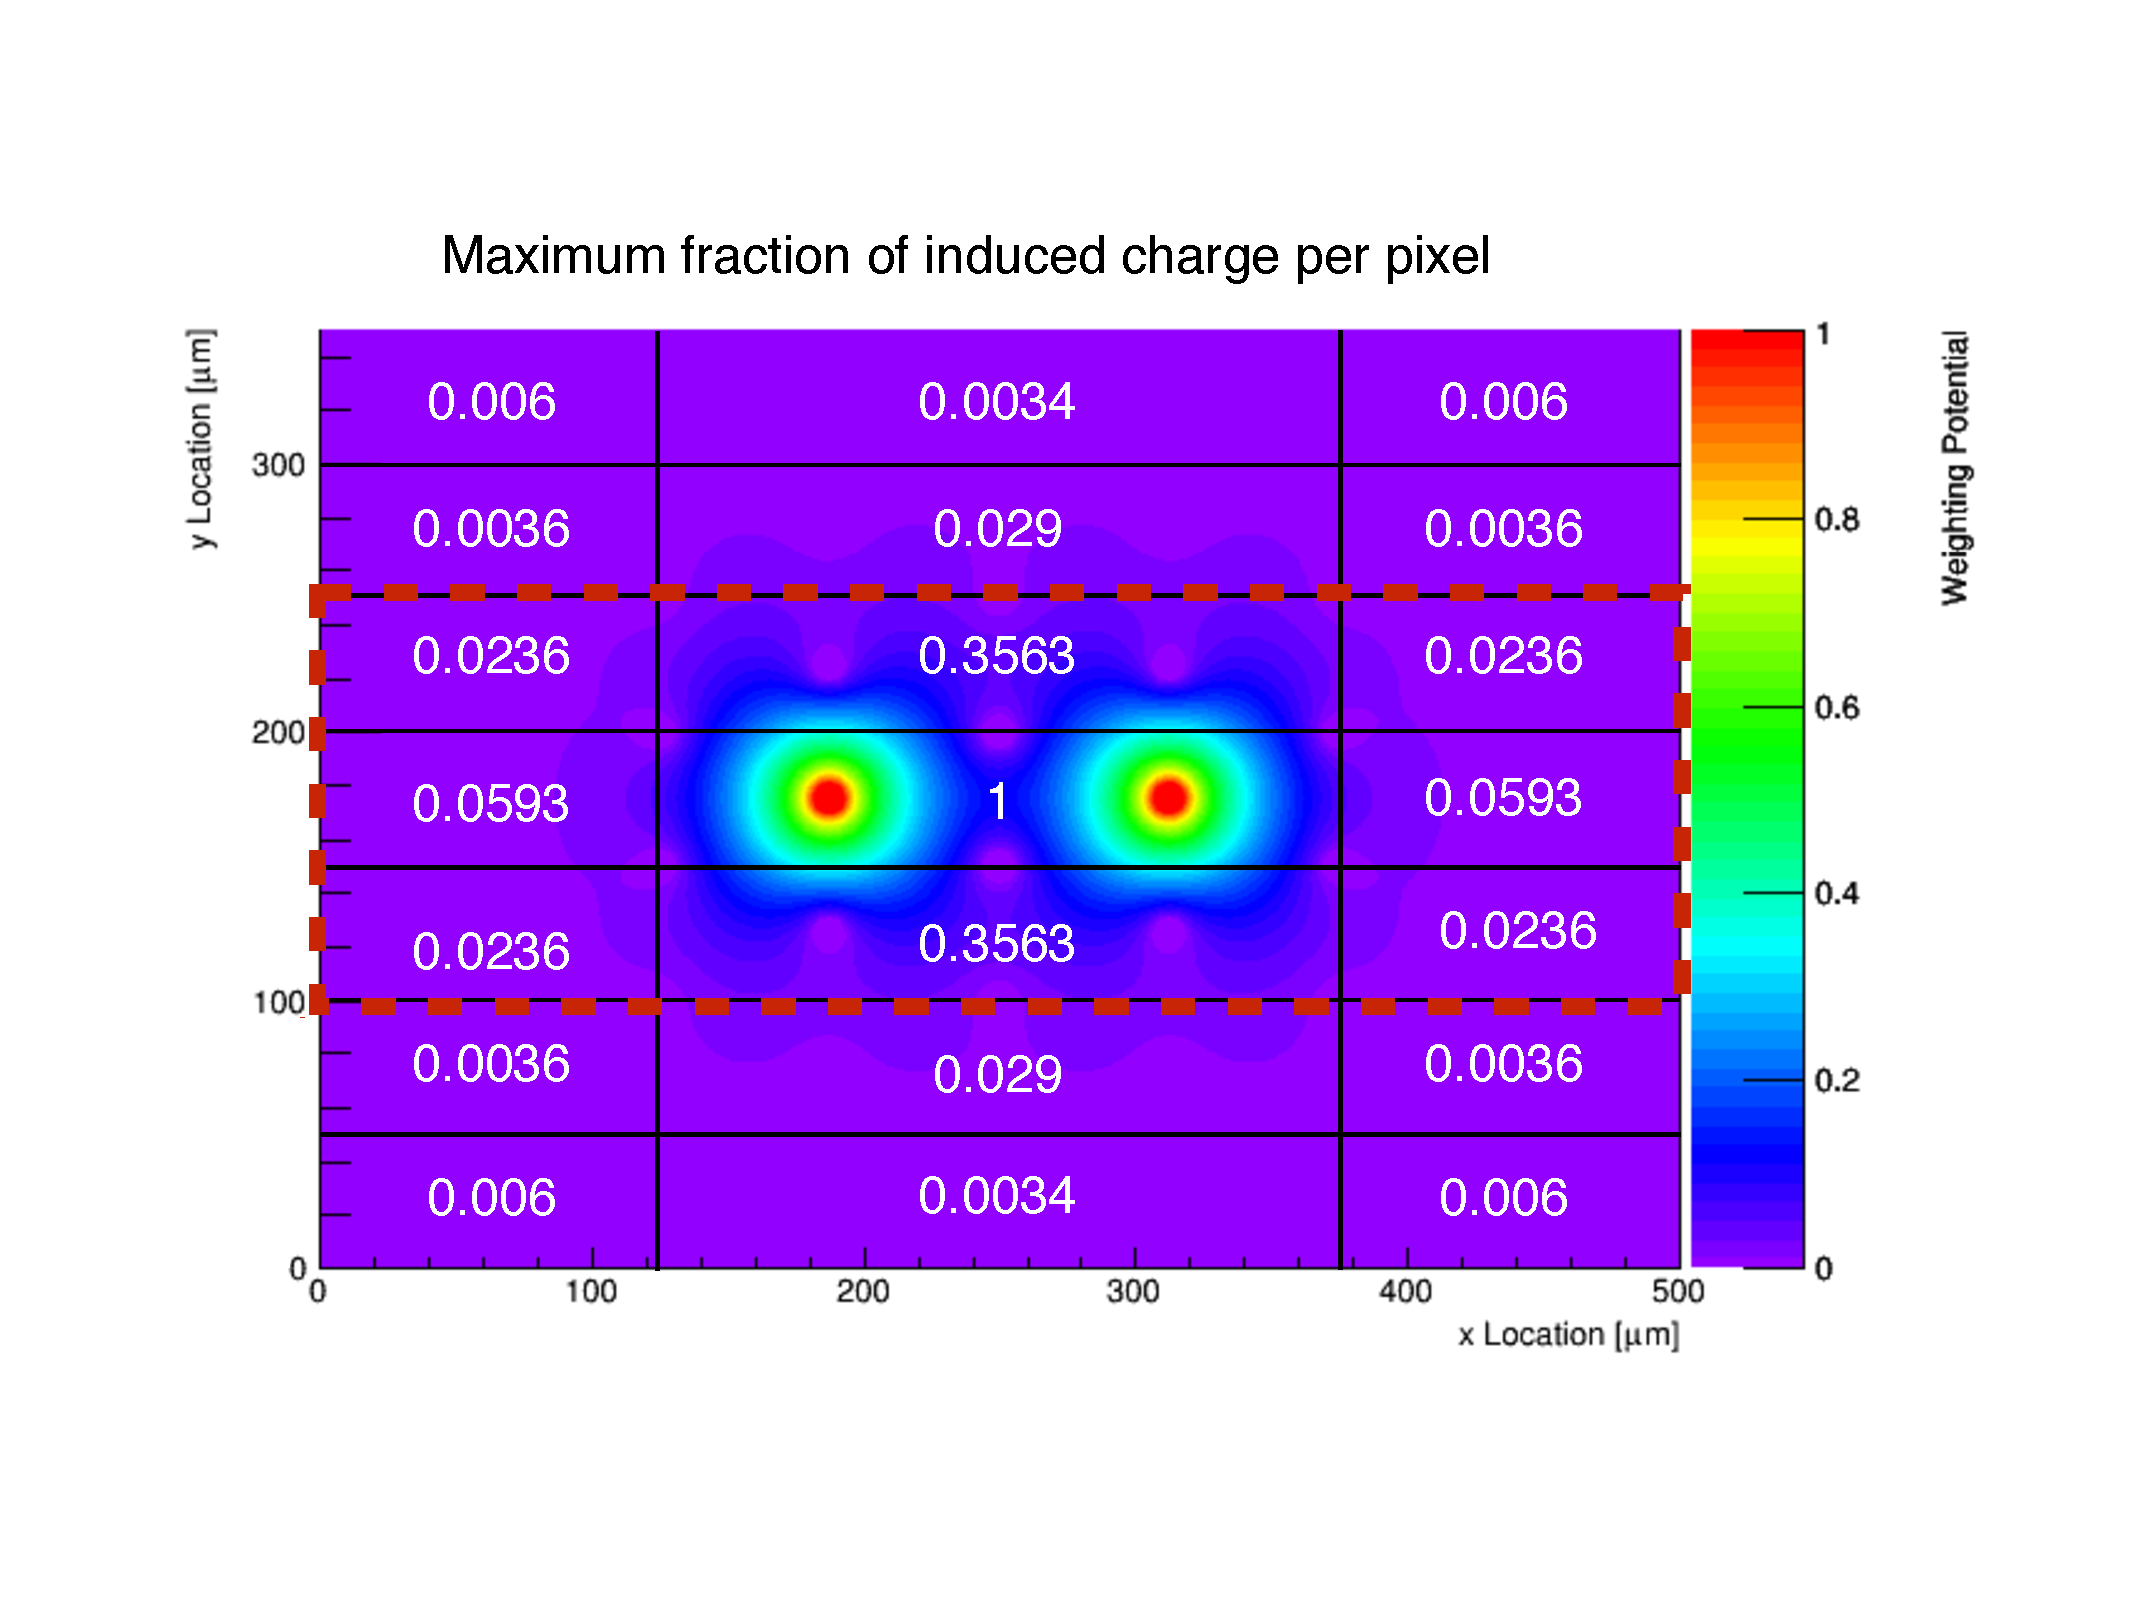
\includegraphics[width=0.6\textwidth]{Maximum3D_mod.pdf}
\caption{The Ramo potential for an ATLAS 3D sensor as computed with TCAD.  The two $n^+$ electrodes of the center pixel are electrically connected and therefore both are held at unit potential in the calculation of the Ramo potential.  The circular holes are due to the $p^+$ electrodes.  White numbers indicate the maximum induced charge (normalized to one electron charge) in that pixel considering all starting positions and trapping times.  A red dashed rectangle shows which pixels are included in the simulation.}
\label{fig:ramo:3D}
\end{figure}

\subsection{Charge Chunking}
\label{sec:chunking}

One final component of the digitization model is the treatment of charge chunks.  Approximately 80 electron-hole pairs are generated per micron; it is too computationally expensive to individually propagate each one of these.  Therefore, chunks of charge, representing many fundamental charge carriers are propagated through the digitization code.  While the average collected charge from a chunk is the same as for individual charge carriers, the fluctuations in the induced charge can be significantly over-estimated.  This is corrected by \textit{unsmearing} the fluctuations.  This is possible if the mean collected charge can be computed ahead of time.  Then, $Q\rightarrow \langle Q\rangle+\frac{1}{\sqrt{n}}(Q-\langle Q\rangle)$ will have the correct fluctuation size when $n$ is the number of fundamental charges represented by one charge chunk.  The average charge $\langle Q\rangle$ can be computed by running the simulation many times, or approximated analytically by the following formula:

\begin{align}\nonumber
\label{eq:chukingwithtrapping}
\langle Q_\text{collected}\rangle&=\langle Q_\text{collected}^\text{electrons}+Q_\text{collected}^\text{holes}\rangle=\\\nonumber
&Q\int_0^\infty dz p^e(z_0\rightarrow z) (\phi(z)-\phi(z_0))+Q\int_0^\infty dz p^h(z_0\rightarrow z) (\phi(z)-\phi(z_0))\\\nonumber
&=Qe^{-t_e/\tau_e}(\phi(L)-\phi(z_0))-Qe^{-t_h/\tau_h}(\phi(0)-\phi(z_0))\\
&\hspace{4mm}+Q\int_{z_0}^L dz p^e(z_0\rightarrow z) (\phi(z)-\phi(z_0))-Q\int_{z_0}^0 dz p^h(z_0\rightarrow z) (\phi(z)-\phi(z_0)),
\end{align}

where $p^{e/h}(z_0\rightarrow z)$ is the probability density for an electron or hole to drift from $z_0$ to $z$ and be trapped at $z$.  Figure~\ref{fig:chunking:correction} illustrates the impact of the charge chunking correction when applied to electrons in a 3D sensor for $\Phi=10^{16}$ $n_\text{eq}/\text{cm}^2$.  Charge that reaches the electrode without being trapped as well as the charges that are trapped and only contribute via the Ramo potential are addressed by this correction.

\begin{figure}[!htpb]
\centering
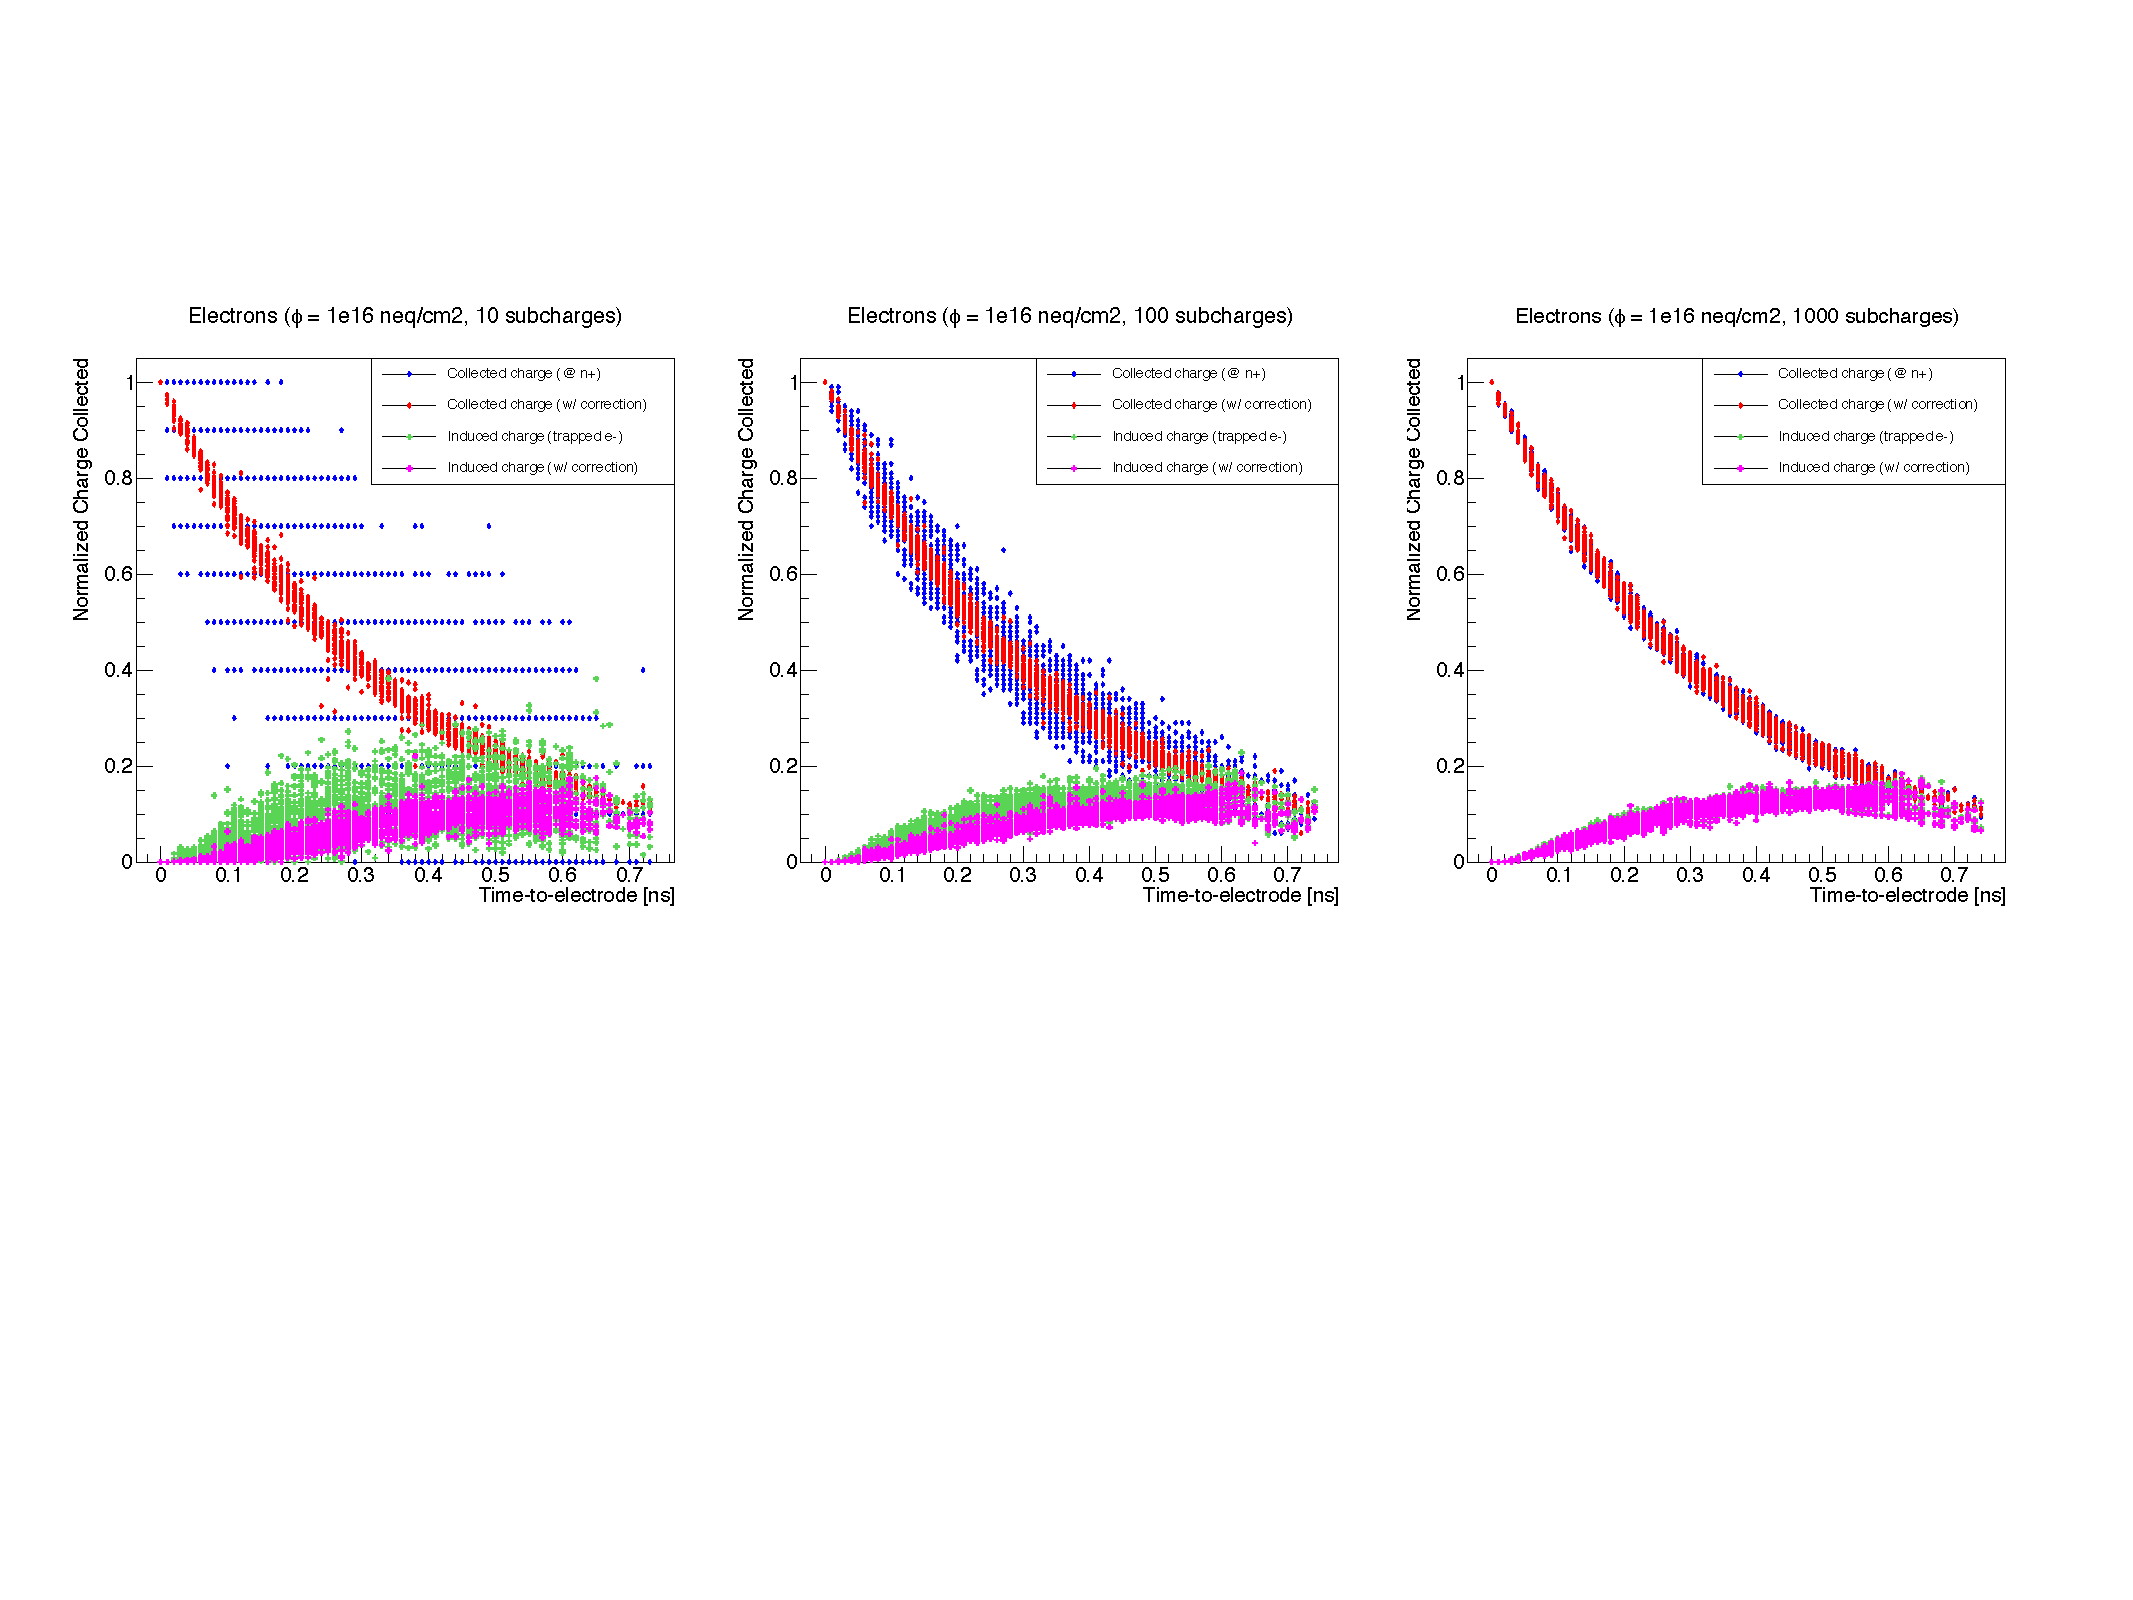
\includegraphics[width=0.9\textwidth]{chunking3D.pdf}
\caption{An illustration of the charge chunking correction applied to the charge collection in 3D sensors with $\Phi=10^{16}$ $n_\text{eq}/\text{cm}^2$.  The initial energy deposited by Geant4 is split into 1000 (right), 100 (middle), or 10 (left) sub-charges; correspondingly, the number of fundamental charge carriers per chunk increases from right to left.  The red and purple in all three plots shows the corrected distributions while the blue and green are the uncorrected distributions.  In the right plot, the correction does very little, while it is a significant correction for the left plots.}
\label{fig:chunking:correction}
\end{figure}

\section{Full Digitizer Predictions and Validation}
\label{sec:digivalidation}


\subsection{Data and Simulation}

%https://twiki.cern.ch/twiki/bin/view/Atlas/PixelConditionsRUN2
Given the models presented in the previous sections, it is critical to validate the physics as well as the implementation by comparing the simulations with data.  This section presents two key observables for studying radiation damage: the charge collection efficiency and the Lorentz angle.  These two quantities are measured as a function of time in Run 2 for the innermost pixel layer, which was installed during the shutdown between runs and thus was unirradiated at the start of Run 2.  The data were collected in the fall of 2015 and throughout 2016 with single muon triggers.  Charged particle tracks are reconstructed from hits in the Pixel detector, silicon strip detector, and transition radiation tracker.  Clusters on the innermost pixel layer associated to tracks are considered for further analysis.  The IBL is operated at 80 or 150 V at a temperature of 70 K in 2015 and 288 K in 2016.  The analog threshold is 2550 e with 4 bits of ToT for the digital charge readout.  The ToT is calibrated so that a ToT of 8 corresponds to 20 ke and a digital threshold of ToT $>1$ is applied.  The ADC is modeled in simulation using the same charge to ToT conversion.

Simulated datasets are based on Geant4~\cite{Agostinelli:2002hh} with digitization implemented in the full ATLAS simulation framework (ATHENA)~\cite{Aad:2010ah} or a standalone package called Allpix~\cite{benoit:20xx}.  The later is a lightweight wrapper of Geant4 that is optimized for testbeam analysis and is a powerful test-bench for digitizer development.

%user.stsuno.mc15 13TeV.361107.PowhegPythia8EvtGen AZNLOCTEQ6L1 Zmumu.2015.v01 EXT2 for the simplified?

\subsection{Charge Collection Efficiency}
\label{sec:CCE}

The collected charge is represented by the mode of the charge distribution, which is approximately Landau~\cite{Landau:1944if}.  The charge collection efficiency is defined to be the collected charge at one fluence divided by the charge for unirradiated sensors in overdepletion.  Figure~\ref{fig:CCE:Run2} shows the measured and predicted charge collection efficiency as a function of integrated luminosity in Run 2. Data points are corrected in order to account for the drift in the ToT calibration, as it can be seen in figure \ref{fig:ToTCalibrationDrift}, where the mean and RMS evolution of the ToT for all the IBL modules is shown, as measured in calibration scans. The tuning point was 10  for 16k electrons for 2015 and 8 for 2016. Radiation effects are assumed to cause the measured ToT to drift  with integrated luminosity, but short periods of annealing and regular re-tunings brought the mean ToT back to the tuning point. The drift is assumed linear between calibration and the correction is evaluated in the middle of the run considered. To this correction is assigned an error of 30 \% (which is then propagated to the charge collection efficiency value. MPV value of the fitted Landau distribution are then scaled up or down (accordingly to the direction of the drift). This effect depends run by run, but is in general below 5\% with a final error on the measure of $\sim 2/3 $ \%. The error on the predicted value of the charge collection efficiency is evaluated by taking the squared sum of the differences between the nominal value and the one obtained with the variation of the radiation damage parameters, as explained in detail in section \ref{sec:Efieldmodelcomparisons}. In addition is also considered a variation of the trapping probability constant of 10\% up and down. An error of 3\% is also assigned to the luminosity value of the data points (the horizontal error bars in figure \ref{fig:CCE:Run2}). Instead, for the Allpix simulation points, the integrated luminosity is converted to a fluence using the information presented in Fig.~\ref{fig:fluenceoverview}, and an error of 15\% is assigned to the conversion. As expected, the efficiency drops with fluence due to charge trapping.  A breakdown of the impact of the systematics variations is reported in table \ref{tab:SystError}. The simplified model tends to over-predict the collected charge, in part because it ignores the non-trivial dip in the electric field in the center of the sensor.   Approximate predictions for the outer pixel layers and projects for the 2017 run are presented in Appendix~\ref{sec:additional}.

\begin{figure}[!htpb]
\centering
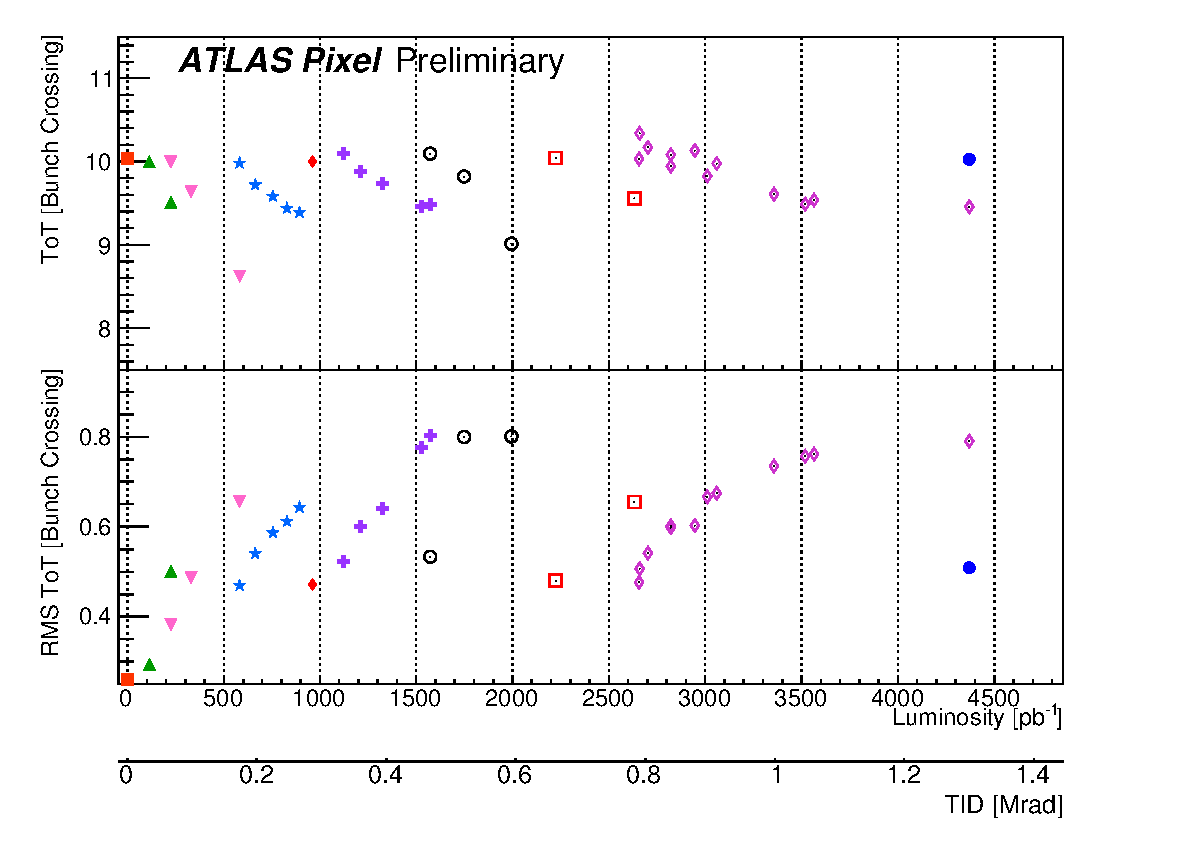
\includegraphics[width=0.45\textwidth]{2015Calibration.pdf}
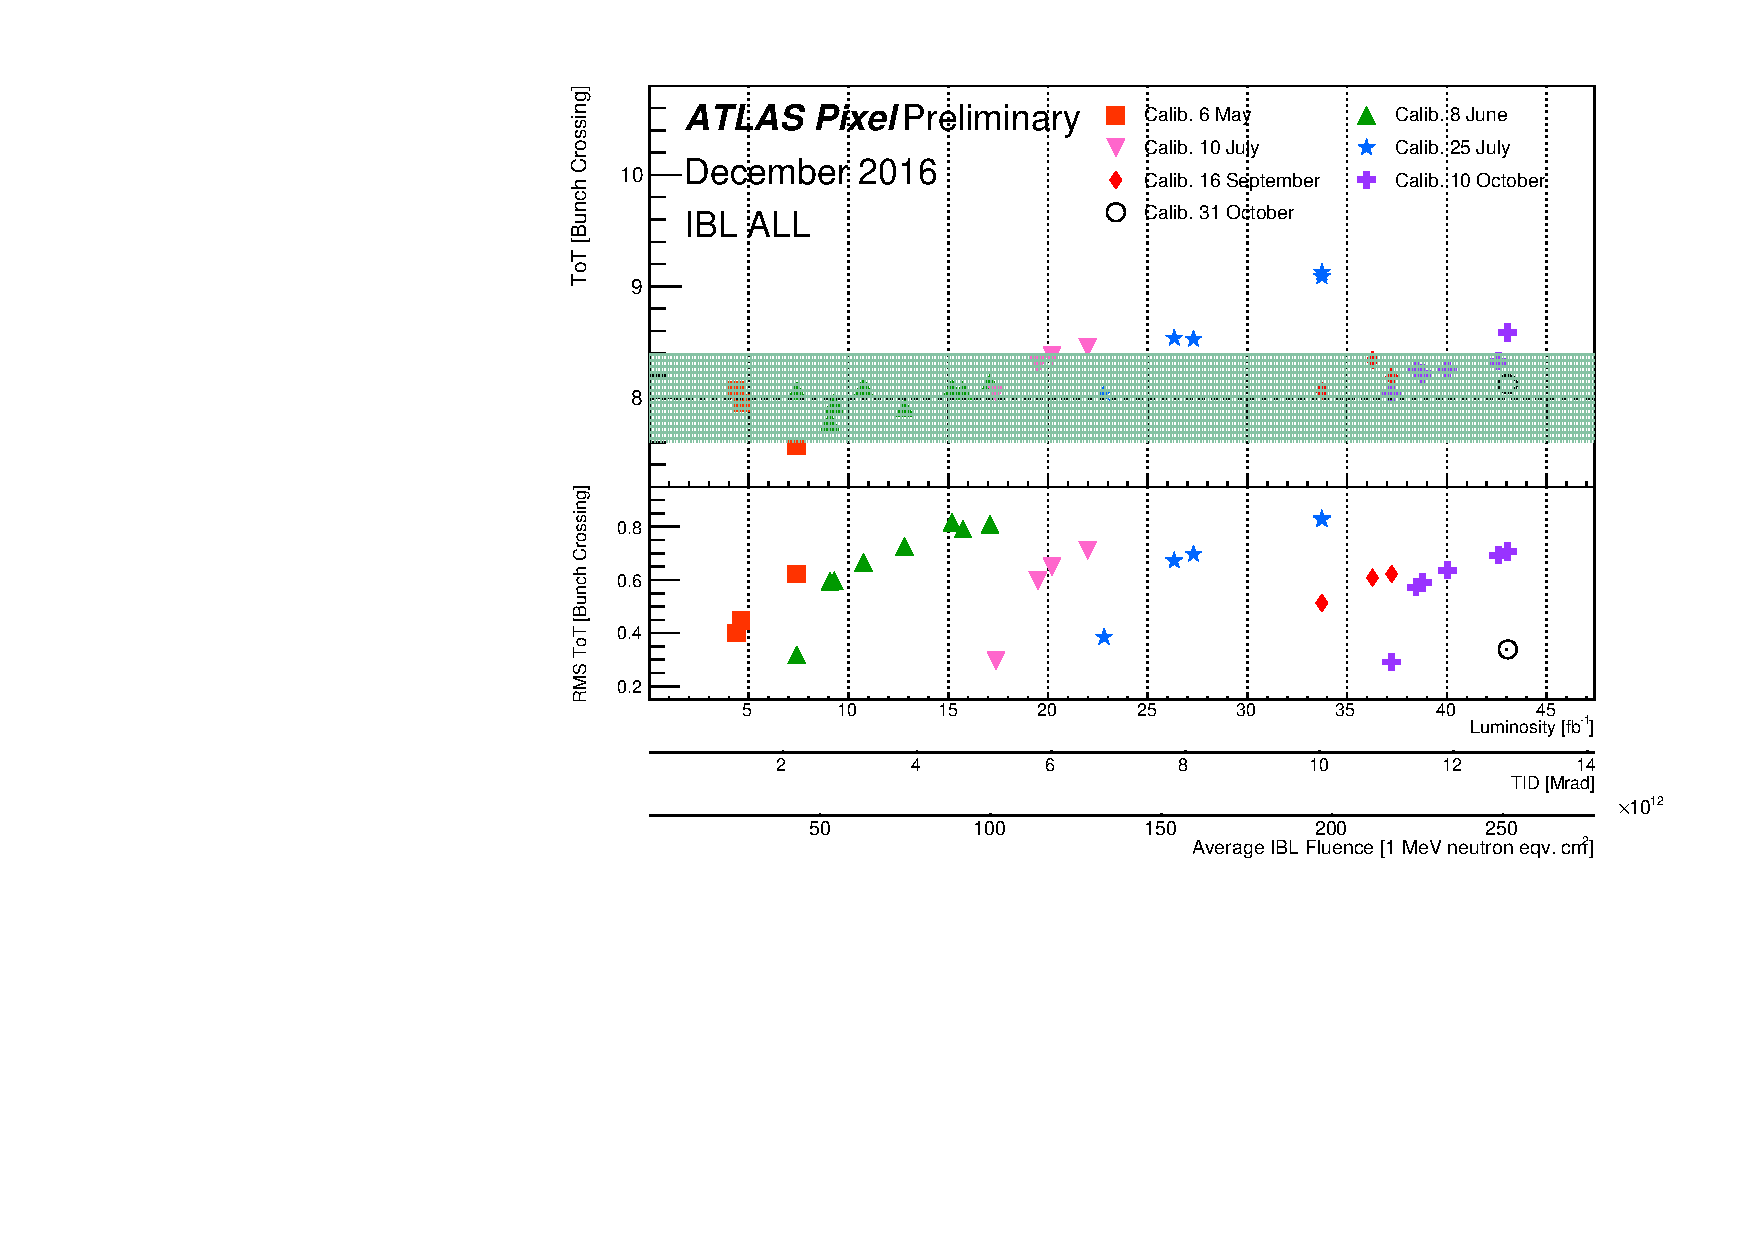
\includegraphics[width=0.45\textwidth]{2016Calibration.pdf}
\caption{The evolution of the mean and RMS of the measured Time-over-Threshold (ToT) over all pixels in the IBL detector as a function of the integrated luminosity and the corresponding total ionizing dose (TID) in 2015 (left) and 2016 (right), as measured in calibration scans. Each color/symbol series corresponds to a single tuning of the detector. }
\label{fig:ToTCalibrationDrift}
\end{figure}


\begin{figure}[htpb!]
\centering
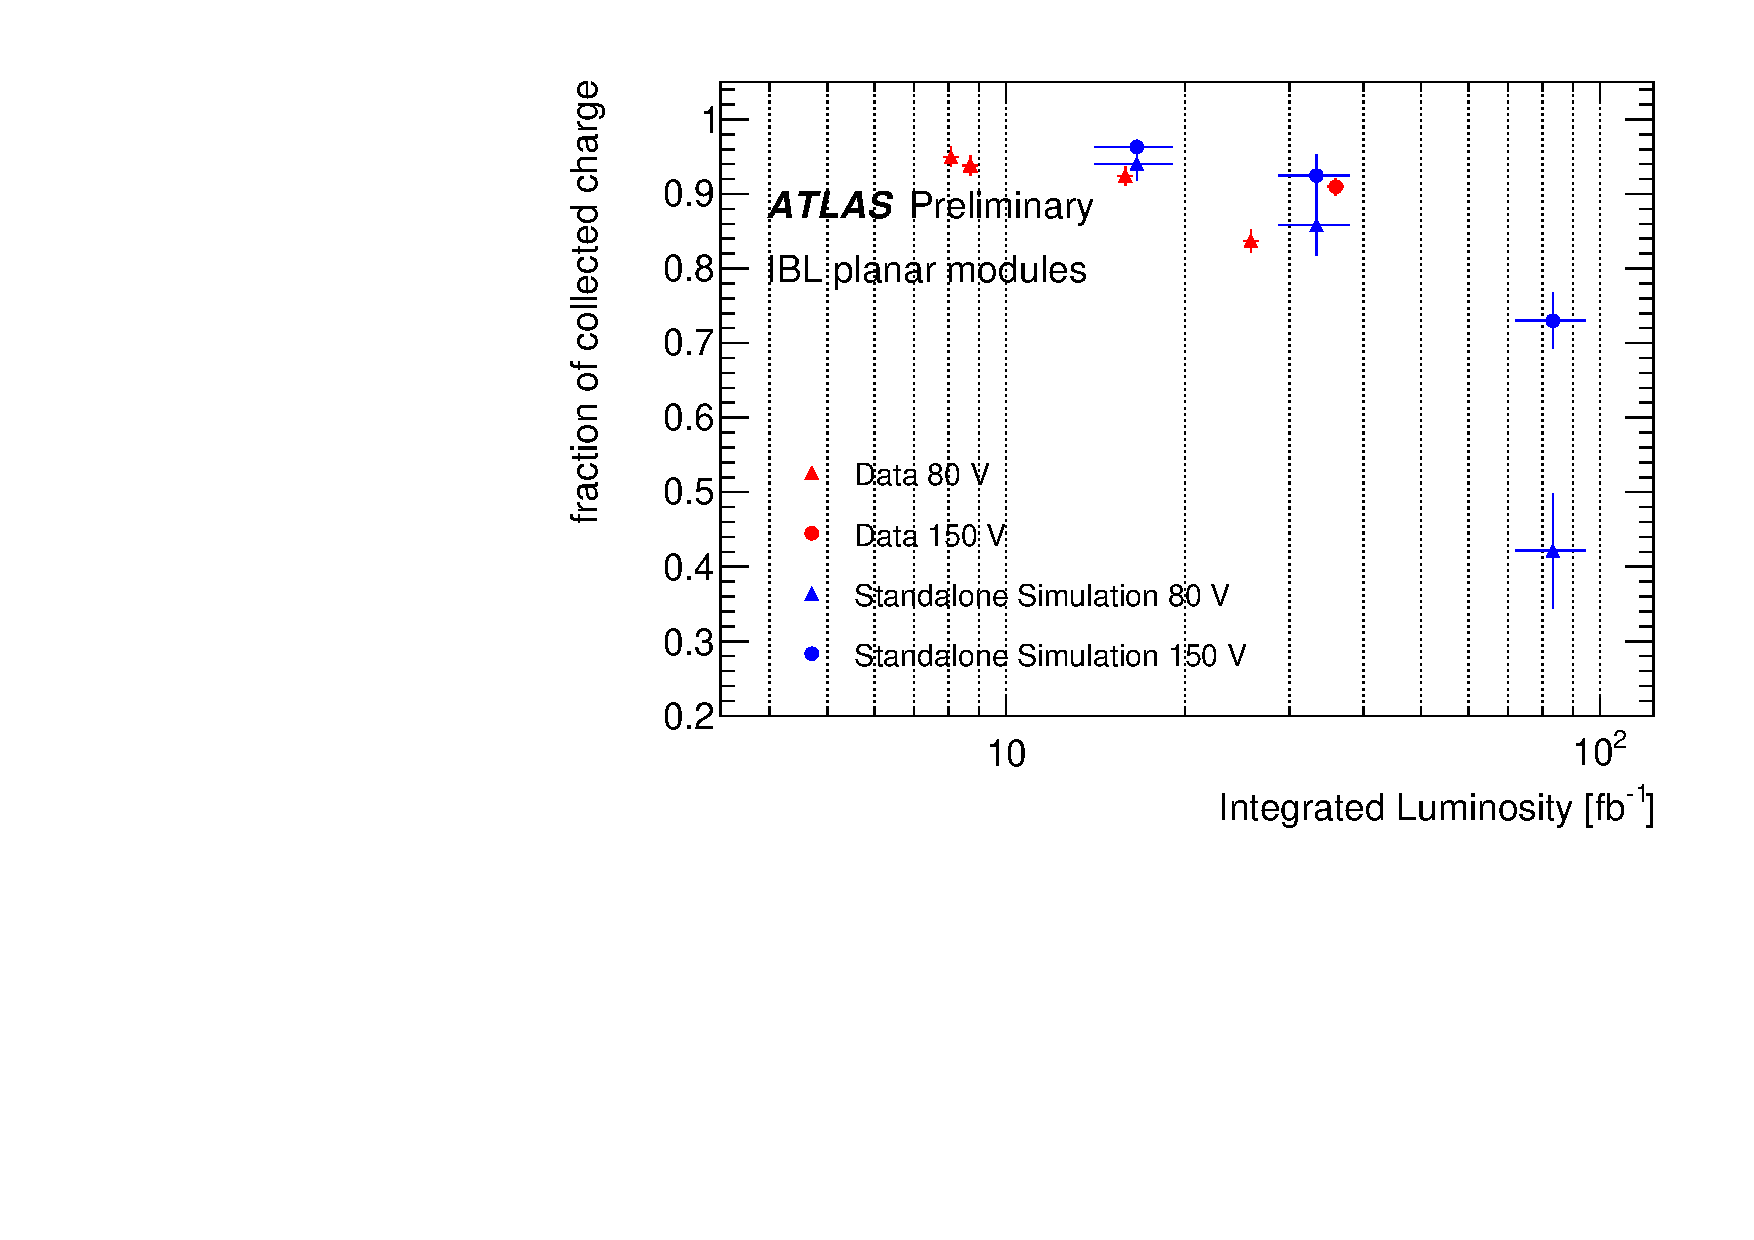
\includegraphics[width=0.65\textwidth]{CCE_Run2_approved.pdf}
\caption{The charge collection efficiency as a function of integrated luminosity.}
\label{fig:CCE:Run2}
\end{figure}



\begin{table}[!htpb]
\begin{center}
\setlength{\tabcolsep}{0.0pc}
{\tiny
%%
\begin{tabular*}{0.7\textwidth}{@{\extracolsep{\fill}}lrrrrrr}
%\noalign{\smallskip}\hline\noalign{\smallskip}
 %       & \bf{SR }             \\[-0.05cm]
\noalign{\smallskip}\hline\noalign{\smallskip}
%%
%%
%%
bias Voltage [V]		& 80 & 80 & 80& 150 & 150 &150\\
fluence 					& 1 & 2 & 5 & 1 & 2 & 5\\
\noalign{\smallskip}\hline\noalign{\smallskip}

Variation 				& impact [\%] & impact [\%] & impact [\%] & impact [\%]& impact [\%] & impact [\%]\\
\noalign{\smallskip}\hline\noalign{\smallskip}

Energy acceptor $+10\%$   		& 0.42  	& 2.23  &0.76 & 0.21 & 1.57   &1.51  \\
Energy donor $+10\%$  			& 0.55  	&  -    & 4.46 & 0.16 & 0.35  &5.67\\
Energy acceptor $-10\%$  		& - 		&  1.68 & 3.77& 0.09  & 0.31  & 1.60 \\
Energy donor $-10\%$			& 0.47  	& 0.14  & 2.91 & 0.10  & 0.90 & -\\
\noalign{\smallskip}\hline\noalign{\smallskip}


$\eta$  acceptor $+10\%$  		& 0.43  	& 0.33   & 3.77   & 0.12  & 0.87  &1.28\\
$\eta$  donor $+10\%$  			& 0.25  	& 0.96   & 4.22   & 0.14  & 0.40  &5.72\\
$\eta$  acceptor $-10\%$  		& 0.27  	& 1.71   & 13.83 & 0.06  & 0.29   &1.54 \\
$\eta$  donor $-10\%$ 			& 0.03 	& 0.41   & 6.82   & 0.14  & 0.67   &6.87\\
\noalign{\smallskip}\hline\noalign{\smallskip}

$\sigma_e$ acceptor $+10\%$  	& 0.30		& 1.39   & 0.88 & 0.06 & 0.37  & 2.36\\
$\sigma_e$  donor $+10\%$  		& 0.25  	& 1.01   & 1.81 & 0.01 & 0.38   & 0.65 \\
$\sigma_e$  acceptor $-10\%$  	& 0.44  	& 0.33   &1.91 & 0.12  & 0.84   &4.70\\
$\sigma_e$  donor $-10\%$ 			& 0.13  	& 0.65   & 0.12 & 0.11 & 0.61  &5.53 \\

\noalign{\smallskip}\hline\noalign{\smallskip}

$\sigma_h$ acceptor $+10\%$  	& 0.34  	& 1.55  & 1.33 & 0.12 & 0.83  & 2.64\\
$\sigma_h$  donor $+10\%$  		& 0.28  	& 0.09  & 1.41 & 0.11 & 0.57  &5.04\\
$\sigma_h$  acceptor $-10\%$  	& 0.30  	& 1.96  & 0.95 & 0.08 & 0.33  &2.17\\
$\sigma_h$  donor $-10\%$ 			& 0.29  	& 0.55  & 0.76 & 0.015  & 0.32  &0.83 \\
\noalign{\smallskip}\hline\noalign{\smallskip}
trapping constant $+10\%$ 			& 0.68  	& 2.25  & 3.56 & 1.24 & 1.10 & 1.34 \\
trapping constant $-10\%$  			& 0.60  	& 0.10  & 8.83 & 0.14 & 0.37 &  7.20\\
\noalign{\smallskip}\hline\noalign{\smallskip}
total error 					& 2.36		& 5.20 & 20.41 & 1.37 & 2.98  &16.47\\
%1.0-3.0    &    1.73 $\pm$ 1.43 & 1.28 $\pm$ 1.22\\
\noalign{\smallskip}\hline\noalign{\smallskip}
\end{tabular*}
   \caption{List of systematics considered in the errors in the simulation and their relative impact on the nominal value}
   \label{tab:SystError}
%%%%
}
\end{center}

\end{table} 


\subsection{Lorentz Angle}
\label{sec:lorentzangle}

The Lorentz angle is defined as the transverse incidence angle corresponding to the minimum cluster size.  The angle is determined precisely by performing a fit to this distribution using the following functional form:

\begin{align}
F(\alpha)=[a\times(\tan\alpha-\tan\theta_L)+b/\sqrt{\cos\alpha}]\oplus G(\alpha),
\end{align}

where $\alpha$ is the incident angle, $\theta_L$ is the Lorentz angle, and $a$ and $b$ are two fit parameters.  The fitted Lorentz angle as a function of integrated luminosity is shown in Fig.~\ref{fig:LA2:Run2}.  Due to the degradation in the electric field, the mobility and thus Lorentz angle increases with fluence.  Charge trapping does not play a significant role in the Lorentz angle prediction - the full radiation damage model but with a constant electric field predicts no fluence dependence of the angle.

\begin{figure}[h!]
\centering
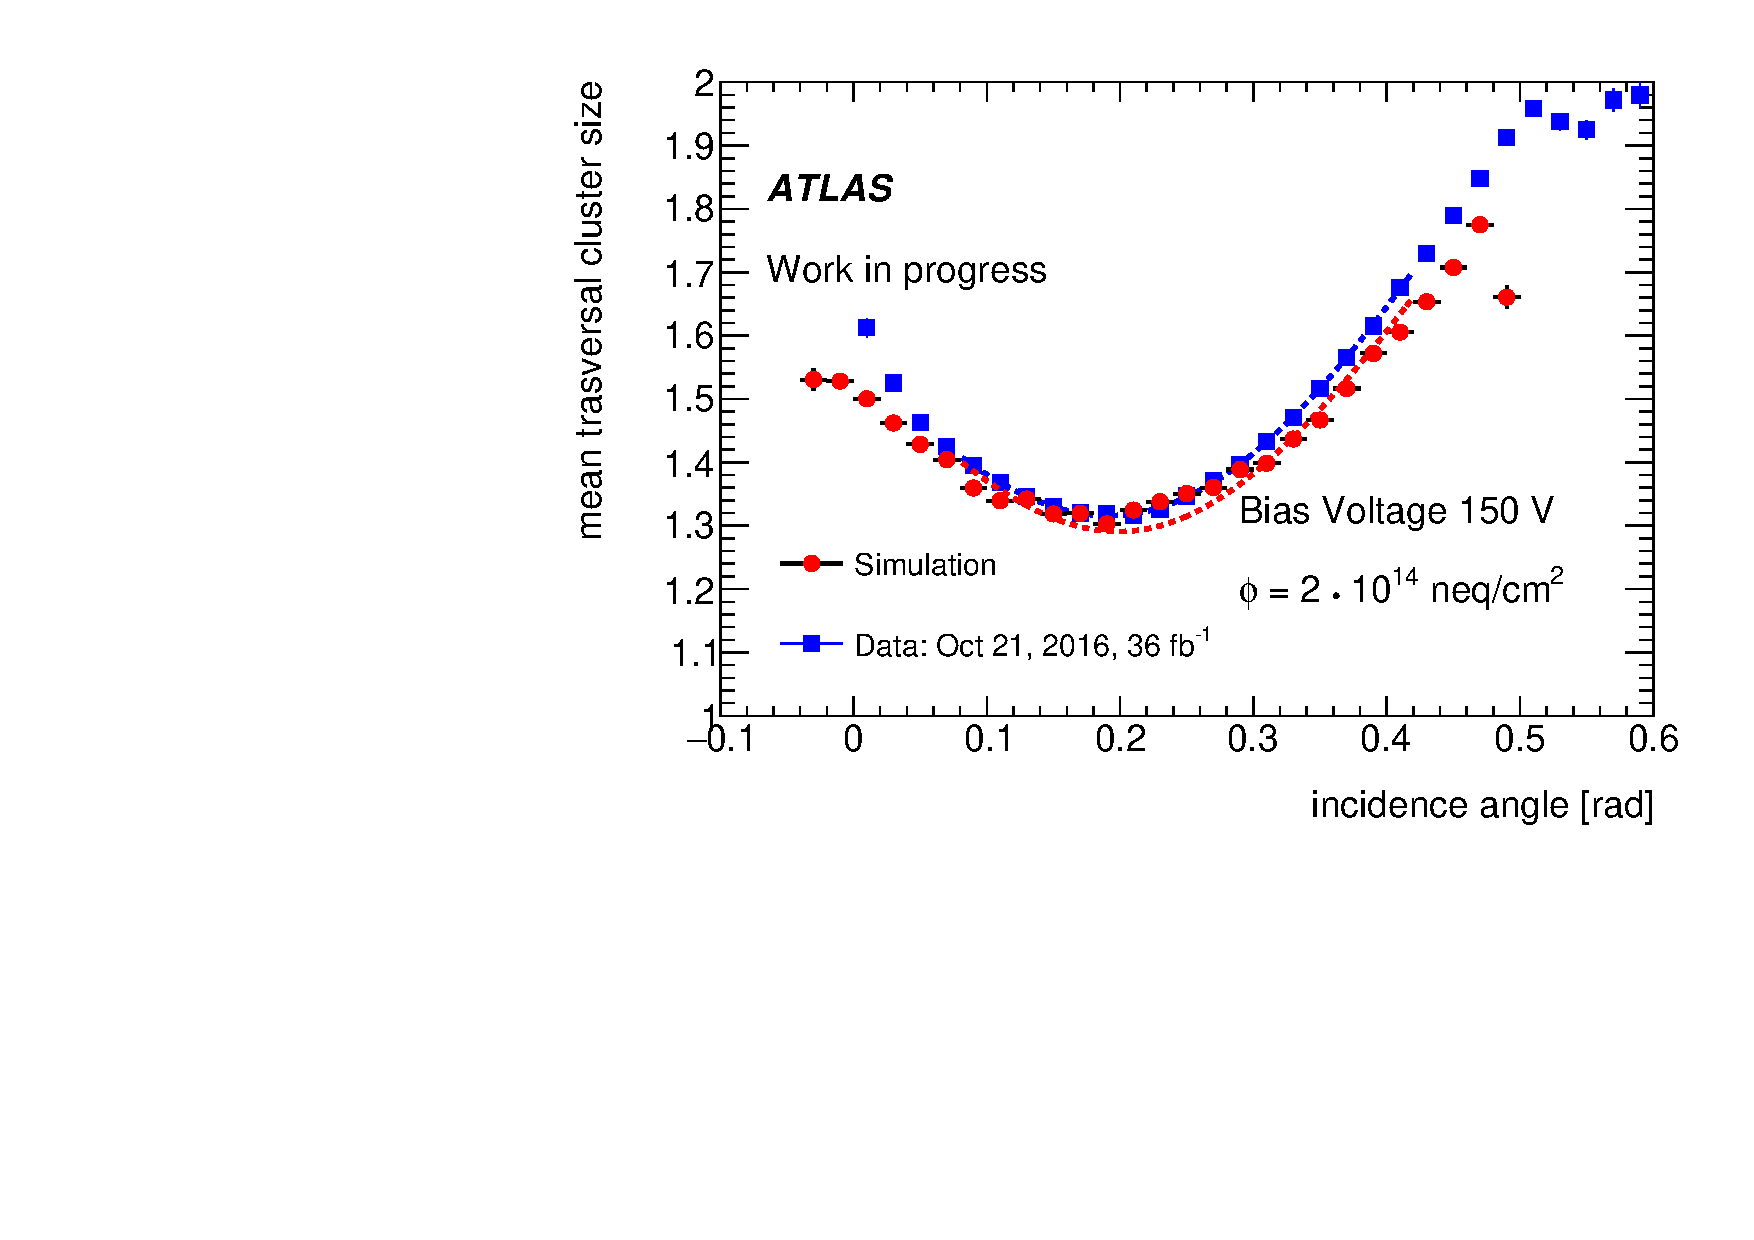
\includegraphics[width=0.5\textwidth]{profile_rad_sizeX_debug_f2e14_V150_BenMap_100k_2x2_mapLorentzOK_311071_Chiocchia_withdate_and_lumi.pdf}
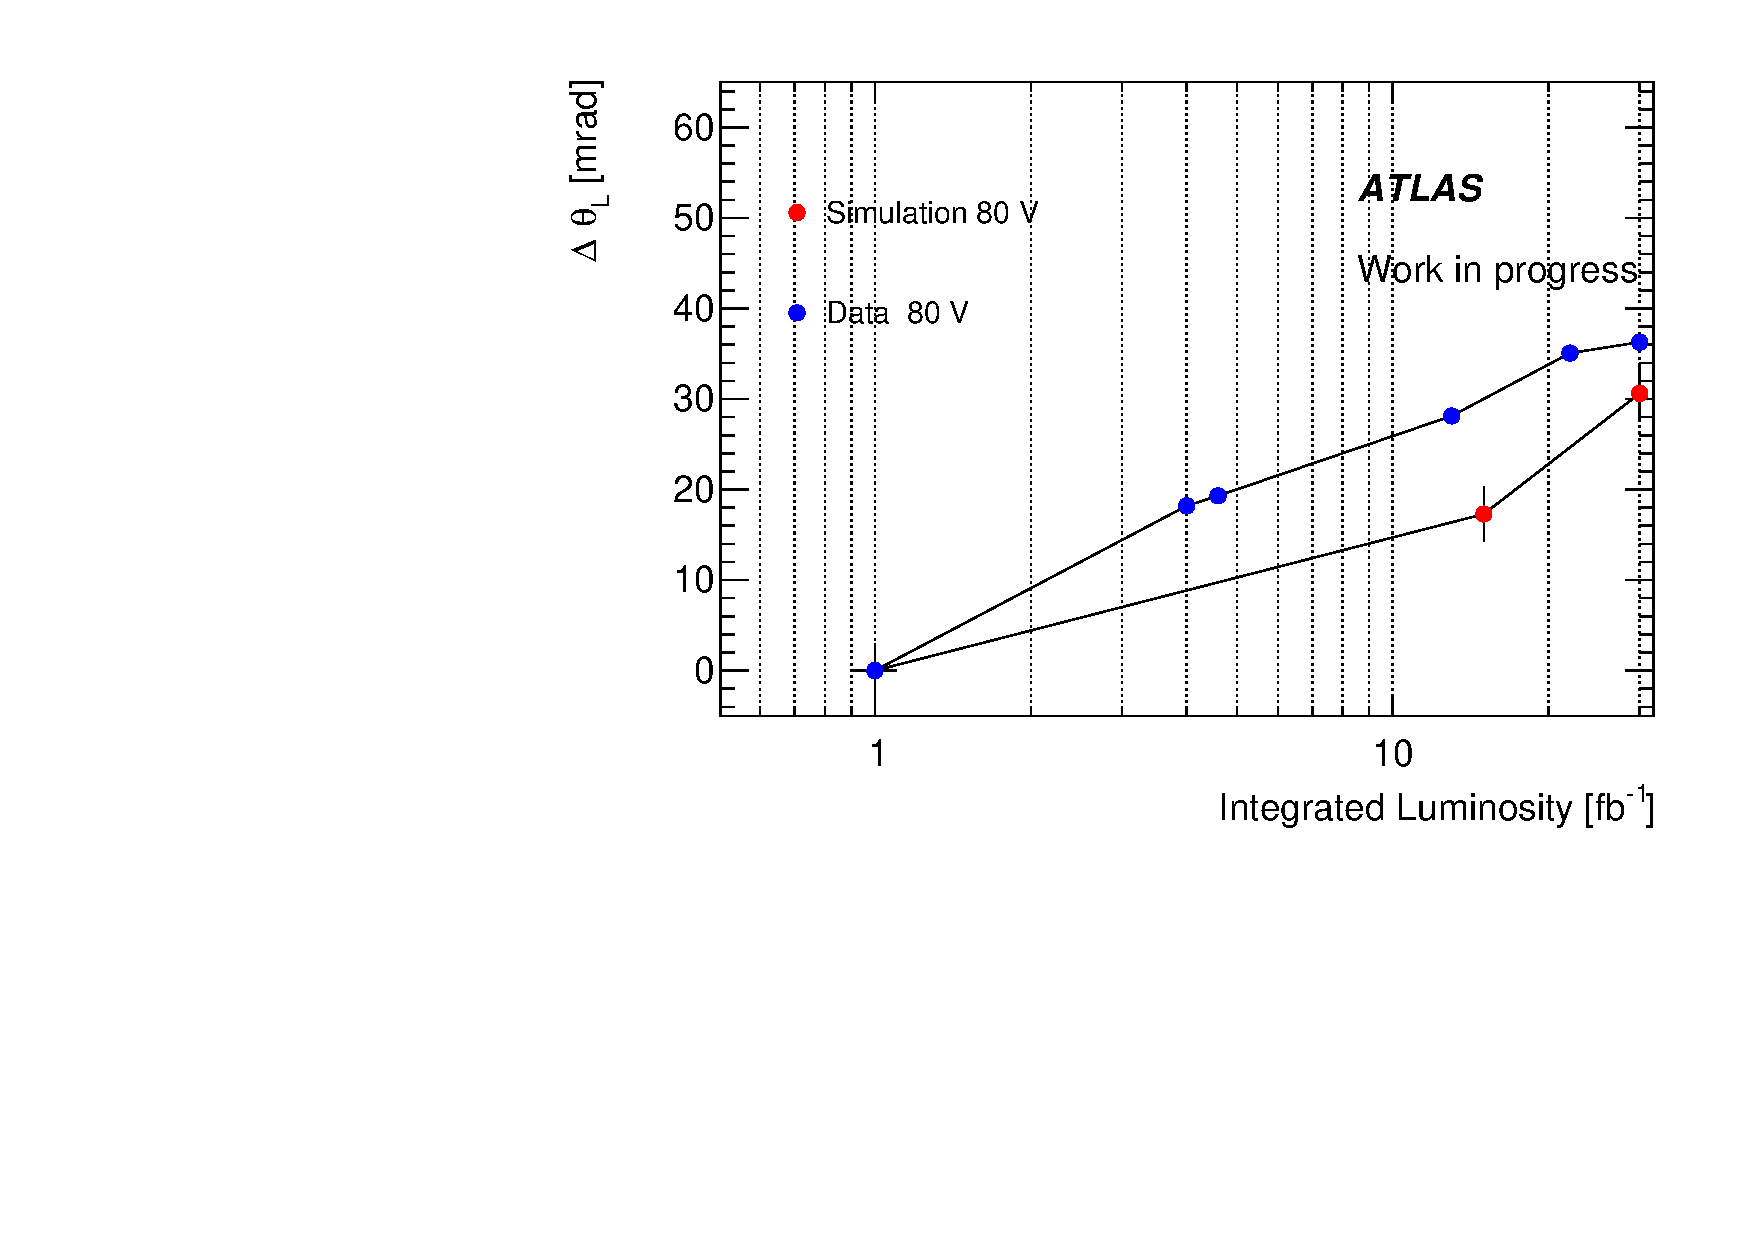
\includegraphics[width=0.5\textwidth]{MultiProfile_LorAngVsLumi_03_45.pdf}
\caption{Left: the mean transverse cluster size versus transverse incidence angle near the end of the 2016 run ($\sim2\times 10^{16}$ $n_\text{eq}/\text{cm}^2$) with a bias voltage of 150 V.  Right: The Lorentz angle as a function of the integrated luminosity.}
\label{fig:LA2:Run2}
\end{figure}






\section{Full Digitizer: Summary and Perspectives}
\label{sec:digiconclusions}



This Chapter presents a digitization model for ATLAS planar and 3D sensors that includes radiation damage effects.  In addition to describing the physics processes incorporated in the digitizer, two key observables are studied using Run 2 data to show excellent agreement between the simulation and the observations. The focus here was on Run 2 and 3 conditions, but the models can be used to make important design decisions for the upgraded ATLAS detector that must survive the harsh HL-LHC radiation environment.


